\documentclass[letterpaper,twocolumn,10pt]{article}
\usepackage{usenix,epsfig,endnotes}
\usepackage{cite}
\usepackage{amsfonts,amsmath, amsthm}
\usepackage{xspace}
\usepackage{pifont}
\usepackage[usenames,dvipsnames]{color}
\usepackage{multirow}
\usepackage[english]{babel}
\usepackage{graphicx}

\usepackage{authblk}
%\usepackage{diagbox}
\newtheorem{definition}{Definition}
\newtheorem{theorem}{Theorem}
\newtheorem{corollary}{Corollary}
\newtheorem{lemma}{Lemma}
\newtheorem{fact}{Fact}
\newtheorem{proposition}{Proposition}
\newtheorem{claim}{Claim}

\usepackage{wrapfig}
\usepackage{graphicx}
%\usepackage[pdftex]{color} % Force PDF output
\usepackage{caption}

%\usepackage[margin=1in]{geometry}
\usepackage{fancybox}
\usepackage{calc}
\usepackage{url}
\usepackage[hang,scriptsize,tight,nooneline]{subfigure}
\usepackage{algorithm}
\usepackage[noend]{algpseudocode}
%\usepackage{algorithmic}
\usepackage{booktabs}
\usepackage{times}
\usepackage{enumitem}
\makeatletter
\makeatother

\usepackage[compact]{titlesec}

\titlespacing\section{0pt}{2pt plus 2pt minus 2pt}{2pt plus 2pt minus 2pt}
\titlespacing\subsection{0pt}{2pt plus 2pt minus 2pt}{2pt plus 2pt minus 2pt}
\titlespacing\subsubsection{0pt}{2pt plus 2pt minus 2pt}{2pt plus 2pt minus 2pt}

\pdfpagewidth=8.5 true in
\pdfpageheight=11 true in

%\newcommand{\paragraphb}[1]{\vspace{0.03in}\noindent{\bf #1} }
% Give more separation for now ... we might tighten it up later
\newcommand{\paragraphb}[1]{\smallskip{}\noindent{\bf #1} }
\newcommand{\paragraphe}[1]{\vspace{0.03in}\noindent{\em #1} }

%\newcommand{\pbg}[1]{{\color{Green}#1}}
\newcommand{\pbg}[1]{{{#1}}} 
%\newcommand{\pbgc}[1]{{\color{Green}\bf\em{[pbg: #1]}}}
\newcommand{\pbgc}[1]{{}} 

%\newcommand{\matt}[1]{{\color{blue}{#1}}} 
\newcommand{\matt}[1]{{{#1}}} 
%\newcommand{\mattc}[1]{{\color{blue}\bf\em{[matt: #1]}}} 
\newcommand{\mattc}[1]{{}} 

%\newcommand{\wxzcrnew}[1]{{\color{Purple}{#1}}} 
\newcommand{\wxzcrnew}[1]{{{#1}}} 
\newcommand{\wxzcr}[1]{{{#1}}} 
\newcommand{\wxznew}[1]{{{#1}}} 
\newcommand{\wxz}[1]{{{#1}}} 
%\newcommand{\wxzc}[1]{{\color{Purple}\bf\em{[wxz: #1]}}} 
\newcommand{\wxzc}[1]{{}} 

%\newcommand{\kevin}[1]{{\color{red}{#1}}} 
\newcommand{\kevin}[1]{{{#1}}} 
%\newcommand{\kevinc}[1]{{\color{red}\bf\em{[kevin: #1]}}} 
\newcommand{\kevinc}[1]{{}} 

% http://en.wikibooks.org/wiki/LaTeX/Colors

\newcommand{\cut}[1]{}
% To make the FIXMEs go away, comment out this line...
%\newcommand{\fixme}[1]{{\bf\textcolor{red}{[#1]}}}
% ...and uncomment this one.
\newcommand{\fixme}[1]{}

\newcommand{\parheading}[1]{\medskip{} \noindent \textbf{#1}}

\newcommand{\name}{$CCG$\xspace}
\newcommand{\eps}{\varepsilon}

\captionsetup{font={bf, small}}

\begin{document}

%%%%%%%%%%%%%%%%%%%%%%%%%%%%%%%%%%%%%%%%%%%%%%%%%%%%%%%%%%%%%%%%%%%%%%%%%%%%%%%%



\title{\vspace{-0.24in}\Large \bf Enforcing Customizable Consistency Properties in\\Software-Defined Networks}

% Submission is double blind -- don't show names
%\numberofauthors{1}
%\author{\vspace{-7mm}Paper \#56}
%\author[]{Paper #281, 14 pages}
\author[*]{Wenxuan Zhou}
\author[**]{Dong Jin}
\author[*]{Jason Croft}
\author[*]{Matthew Caesar}
\author[*]{P. Brighten Godfrey}
\affil[*]{University of Illinois at Urbana-Champaign}
\affil[**]{Illinois Institute of Technology}

%\date{~}

\maketitle

\begin{abstract}

It is critical to ensure that network policy remains consistent 
during state transitions. However, existing techniques impose a high
cost in update delay, and/or FIB space. 
We propose the Customizable Consistency Generator (\name), 
a fast and generic framework to support {\em customizable} consistency policies
during network updates.
%under temporal uncertainty about the network state.
\name effectively reduces the task of {\em synthesizing} an update plan 
under the constraint of a given consistency policy to a {\em verification} problem,
by checking whether an update can safely be installed in the network at a particular time,
and greedily processing network state 
transitions to heuristically
minimize transition delay. 
We show a large class of consistency policies
are guaranteed by this greedy heuristic alone;
in addition, \name makes judicious use of existing heavier-weight
network update mechanisms to provide guarantees when necessary.
As such, \name
nearly achieves the ``best of both worlds'': the efficiency
of simply passing through updates in most cases, with
the consistency guarantees of more heavyweight techniques.
Mininet and physical testbed evaluations
demonstrate \name's capability to achieve various types
of consistency, such as path and bandwidth properties,
with zero switch memory overhead and up to a $3\times$
delay reduction compared to previous solutions.



%Modern networks are dynamic. 
%It is critical to ensure that network policy remains consistent during state transitions.
%However, %as networks evolve,
%the inherent distributed and asynchronous nature of networks causes
%any single point incapable to control the exact timing of network events, 
%any single point of the network uncertain about the 
%instantaneous global state to some extent, thus making the problem harder.
%ultimately leading to inconsistency between desired policy and actual network behavior.
%The emergence of Software Defined Networking doesn't change the fact, 
%despite having a logically centralized interface. 
%Existing mechanisms only guarantee some fixed consistency notions, 
%regardless of system requirement and performance overhead.

%We propose the Customizable Consistency Constructor (\name), 
%a fast and generic framework to support {\em customizable} consistency policies
%as networks evolve.
%during network transitions under temporal uncertainty about the network state.
%\name leverages a black-box approach and 
%introduces a graph-based uncertainty-aware network modeling technique.
%\kevin{\name effectively reduces the task of synthesizing an update plan 
%\cut{for preserving}
%\wxznew{under the constraint of} any given consistency policy to a general verification problem.
%We develop a novel network modelling technique allow us to reason networks even under temporal uncertainty, and build our verification engine based on it.
%By checking whether an update can safely be applied in a network at a particular time, the basic scheduling component of \name greedily processes network %state transitions to heuristically minimize transition delay.}
%For a given consistency policy, \name synthesizes an update plan that heuristically minimizes transition delay, \wxznew {by reducing a synthesis problem to a %verification problem.}
%We identify the scope of consistency policies that are guaranteed by that heuristic.
%\name also gives network operators a flexible choice to balance consistency and efficiency during network updates.
%For policies out of that scope, \name triggers a heavyweight plug-in mechanism that guarantees the required policies, when and only when necessary.
%In:addition, \name's greedy update scheduling algorithm can easily be integrated with existing network update mechanisms for significant speed improvements with the same level of consistency enforcement. 
%In that way, \name nearly achieves the ``best of both worlds":
%the efficiency of simply passing through updates in most cases,
%with the consistency guarantees of more heavyweight techniques.
%Both Mininet and physical testbed evaluations demonstrate \name's capability to achieve various types of consistency, such as trace and bandwidth properties, %with close to zero switch memory overhead and up to a factor 3x delay reduction compared to previous solutions.


%The complexity of networks attract more and more efforts to make sure they behave correctly. 
%One way to do so is to verify network-wide data plane state, 
%which utilizes the uniform format of data plane and is able to detect control errors. 
%However, none of the various data plane verification tools take the uncertainty into account.
%They effectively assume that the updates are applied at exactly the moment the they see them.
%In other word, being uncertain of the network status make some bugs neglected.

\end{abstract}

\section{Introduction}
\label{sec:intro}

%\begin{center}
%\emph{"In this world nothing is certain but death and taxes."}
%\end{center}
%\hfill ---{Benjamin Franklin}
%\\

%Modern networks, such as data center networks and enterprise networks, are essential in our daily lives. To keep those networks running properly, network operators often have established a set of correctness conditions.

Network operators often establish a set of correctness conditions to ensure 
successful operation of the network, such as
%Some of those are manually expressed in \wxzcr{configuration files}, such as
%the form of policies, i.e.,
%configurable rules, or regulations on how the network should behave
the preference of one path over another, the prevention of untrusted traffic
from entering a secure zone,
%Others are deemed so obvious they are ``baked in"
%to protocols, such as 
or loop and black hole avoidance. As networks become an increasingly crucial backbone for
critical services,
%such as the power grid, medical networks, military and
%rescue operations, and financial services, and as network operators face
%increasing regulatory requirements on correctness and security
%properties of data transport (e.g., data isolation as in HIPAA, Sarbanes-Oxley,
%etc.), 
the ability to construct networks that obey correctness criteria is becoming
even more important. 
\wxznew{Moreover, as modern networks are in a constant state of changing, it is critical
to keep them correct even during transitions.}
%Unfortunately, today's approach of instilling policies on networks is an
%error-prone process. Operators need to program policies into networks via
%indirect mechanisms (low-level configuration commands on routers), and must
%coordinate actions of complex protocols running across large numbers of
%distributed devices to achieve their network-wide objectives.
%The challenge of constructing networks that work correctly has led to a
%variety of techniques to verify network behaviors~\cite{VeriFlow, PHA2012,
%NetPlumber2013, Anteater2011, Al-Shaer2009, Al-Shaer2010} %, including work on
%configuration analysis~\cite{xx,xx,xx}, flow monitoring~\cite{xx,xx,xx}, and
%reachability modeling~\cite{xx,xx,xx}.  %Those techniques are useful to find
%out when things go wrong, but humans are still involved in the repair process,
%lengthening the time to fix the problem, and introducing potential faults
%during the process.%As networks are dynamic, it is even harder to keep them working correctly.
\wxzcrnew{Thus, the challenge is to guarantee correct transitions, i.e., 
properties are preserved consistently over time, which has been referred as 
%Thus, the challenge is to preserve properties even during
%network state transitions, which we refer to as maintaining 
{\em network consistency}~\cite{Reitblatt2012}.} 
\fixme{This sounds like we came up with the term.  Also this sounds more like correctness than consistency.}

Several recent proposed systems~\cite{Reitblatt2012,incremental-cu,zUpdate, Hong13}
consistently update software-defined networks (SDNs), 
transitioning between two operator-specified network snapshots. However, those
methods maintain only {\em specific} properties, 
and can substantially delay the network update process.
\wxznew{Consistent updates~\cite{Reitblatt2012} (CU), for example, only guarantees
{\em coherence}: during a network update any packet or any flow is
processed by either a new or an old configuration, but never by a mix of the
two. 
%which first instills the new configuration in the middle of the
%network, then updates ingress switches with a flip on packet version numbers.
This is a relatively strong policy that is sufficient to guarantee 
a large class of more specific policies (no loop, firewall traversal, etc.), 
but it comes at the cost of requiring a two-phase update
mechanism that incurs substantial delay between the two phases and doubles flow
entries temporarily. For networks that care only about a weaker consistency property, e.g., only loop
freedom, this overhead is unnecessary.  At the same time, 
networks sometimes need properties \emph{beyond} what CU provides: 
CU only enforces properties on
individual flows, but not across flows (e.g., ``no more than two
flows on a particular link'').
SWAN~\cite{Hong13} and zUpdate~\cite{zUpdate} also ensure only 
a specific property, in their case congestion freedom.} 

That leads to a question: is it possible to efficiently maintain
{\em customizable} correctness policies as
the network evolves?
Ideally, we want the ``best of both worlds'': the efficiency of simply immediately installing updates
without delay, but the safety of whatever correctness properties are relevant to the network at hand.

We are not the first to define this goal.
Recently, Dionysus~\cite{jin2014dynamic} proposed to reduce network update time to just what is
necessary to satisfy a certain property. However, Dionysus requires a
rule dependency graph for each particular invariant, produced by an algorithm
specific to that invariant (the paper presents an algorithm for packet
coherence). For example, a waypointing invariant would need a new algorithm.
Furthermore, the algorithms work only when forwarding rules match exactly one
flow.
% the more complicated case when rules overlap, such as with longest prefix
%match, becomes trivial in \name since checking properties is easy.

We take a very different approach that begins with an observation:
synthesizing consistent updates for arbitrary consistency policies
is hard, but network verification on general policies is comparatively easy,
especially now that multiple real-time data plane verification 
tools~\cite{VeriFlow, Al-Shaer2010, NetPlumber2013}
% \fixme{We cite Al-Shaer; does that paper operate in milliseconds?} 
can verify very generic data-plane properties of a network
state within milliseconds. In fact, as also occurs in domains outside of networking, 
there is a connection between synthesis and verification. 
A feasible update sequence is one which the relevant properties are verifiable at each moment in time.
Might a verifier serve as a guide through the search space of possible update sequences?
%To synthesize a feasible sequence of
%updates to preserve a given invariant, we argue, is to find the timing that each update
%could be scheduled. A general network verifier, on the other hand, 
%is able to tell us whether
%any update is safe to pass to the network at any particular moment by checking
%the supplied invariants. 

Based on that insight, we propose a new consistent update system, 
Customizable Consistency Generator (\name), which efficiently and consistently updates
SDNs under customizable properties (invariants), intuitively by converting the scheduling synthesis problem
to a series of network verification problems.
With \name, network programmers can express desired invariants using an interface (from~\cite{VeriFlow})
which allows invariants to be defined as essentially arbitrary functions of a data plane snapshot,
generally requiring only a few tens of lines of code to inspect the network model. 
Next, \name runs a greedy algorithm: when a new rule arrives from the SDN controller, 
\name checks whether the network would satisfy the desired invariants if the rule were applied. 
%were sent to the relevant device.
If so, the rule is sent without delay; otherwise, it is buffered, 
and at each step \name checks its buffer to see if any rules can be installed safely
(via repeated verifications).

This simplistic algorithm has two key problems.
First, the greedy algorithm may not find the best (e.g., fastest) 
update installation sequence, and even worse,
it may get stuck with no update being installable without violating an invariant.
However, we identify a fairly large scope of policies 
that are ``segment-independent'' for which the heuristic is guaranteed to succeed
without deadlock (\S\ref{sec:seg-independence}).
%That is, to ensure such policies, the heuristic never gets stuck.
For non-segment-independent policies,
\name needs a more heavyweight update technique, 
such as Consistent Updates~\cite{Reitblatt2012} or SWAN~\cite{Hong13}, to act
as a fallback. 
But \name triggers this fallback mechanism only when the greedy heuristic
determines it cannot offer a feasible update sequence.  
This is very rare in practice for the invariants we test (\S\ref{sec:eval}),
and even when the fallback is triggered, only a small part of the transition is 
left to be handled by it, so the overhead associated with the heavyweight mechanism 
(e.g., delay and temporarily doubled FIB entries) is avoided as much as possible.
%In such a way, \name avoids any violation to the desired policies.

The second challenge lies in the verifier.
Existing real-time data plane verifiers, such as VeriFlow and NetPlumber,
assume that they have an accurate network-wide snapshot; 
but the network is a distributed system and we cannot know exactly 
when updates are applied.
%Because of the distributed nature of networks, the \name engine
%is unaware of the precise ordering and timing with which updates arrive at
%devices in the network. However, existing data plane verifiers, such as Veriflow and NetPlumber,
%inaccurately assume the updates applied exact the moment the tools see them.
To address that, \name explicitly models the
uncertainty about network state that arises due to timing,
through the use of \wxzcr{{\em uncertain forwarding graph} (\S\ref{sec:design})}, 
a data structure that compactly represents the range of possible network behaviors
given the available information. 
Although compact, \name's verification engine produces potentially larger models than 
those of existing tools due to this ``uncertainty'' awareness. 
Moreover, as a subroutine of the scheduling procedure, the verification function is called much more frequently
than when it is used purely for verification. For these reasons,
a substantial amount of work went into optimization, as shown in \S\ref{sec:microbenchmark}.

In summary, our contributions are:
\begin{itemize}[noitemsep,topsep=0pt,leftmargin=*]

\item We developed a system, \name, to efficiently synthesize network update orderings 
to preserve customizable policies as network states evolve.

\item We created a graph-based model to capture network \wxzcr{uncertainty}, 
upon which real-time verification is performed (90\% of updates verified within 10 $\mu$s).

\item We evaluate the performance of our \name implementation in both emulation 
and a physical testbed, and demonstrate that \name offers significant performance improvement over previous work---up to $3\times$ faster updates, typically with zero extra FIB entries---while preserving various levels of consistency. 
\end{itemize}
 

\kevin{
%To maximize update speed, we have developed a greedy heuristic scheduling algorithm in \name, and precisely identify the scope of policies whose consistency is completely guaranteed by the heuristic. To make \name capable to handle any given policies, we designed a fallback algorithm that allows \name to fall back from the greedy heuristic to more heavyweight techniques, such as Consistent Updates \cite{Reitblatt2012} and SWAN \cite{Hong13}. \name guarantees such fallback is triggered only when theoretically required, thus preserving strong and flexible consistency properties, with significant reductions in time and memory in practice. Through both emulations and physical testbed experiments, we have demonstrated \name can achieve ...
\kevinc{adding the most promising results here. such as X1-- X2 speedup (or up to X speedup) than previous solutions, memory reduction} }

\if 0
Another key challenge is to achieve a good trade-off between efficiency and consistency.
To this end, \name employs a lightweight heuristic
algorithm as the basic scheduling mechanism, falling back to a more
heavyweight procedure when it encounters cases that are unschedulable
by the lightweight approach.
%To this end, \name employs a greedy heuristic algorithm as the basic scheduling mechanism,
%in order to maximize update speed, 
%and a heavyweight update solution plugged in, to backup the heuristic to guarantee consistency.
We identify the scope of policies that are {\em segment-independent} 
(defined in \S\ref{sec:seg-independence}),
and guaranteed by the heuristic alone.
For non-segment-independent policies, 
\name reliably distinguishes
segment-independent policies, ensuring the lightweight mechanism is
applied whenever possible, yet guaranteeing correctness falling back
to the more heavyweight mechanism when and only when necessary.
%only when the heuristic component determines it cannot offer a 
%feasible update sequence to ensure consistency, \name triggers the plug-in mechanism to proceed updates.
%\fi
%We take a hybrid approach to address the issue. \name is designed in such a way that integration with other update mechanisms, such as Consistent Updates \cite{Reitblatt2012} and SWAN \cite{Hong13}, is straightforward. Such integration is triggered only when the heuristic gets stuck, and thus preserves the consistency level of existing solutions, with significant reduction in time and memory. 
%In this way, \name achieves nearly the ``best of both worlds": the efficiency of passing through updates in most cases, with the consistency guarantees of more heavyweight techniques.
%We demonstrated \name's capability of enforcing generalized consistency properties with high efficiency (in terms of both time and space) through emulations and physical testbed experiments (\S\ref{sec:eval}).

%\if 0
Operators can express\cut{,in a flexible framework,} \wxz{customized} network
properties, and \name ensures that those properties are efficiently
maintained in the presence of network dynamics.  \name works by constructing a
model of distributed network operations, and automatically synthesizing update
sequences to enforce a set of supplied {\em network invariants} \kevin{by verifying the model against the invariants}. A key
challenge is that of dealing with the distributed nature of networks;  the \name engine
is unaware of the precise ordering and timing with which updates arrive at
devices in the network. To address that, \name \cut{(a)} explicitly models the
``uncertainty" about network state through the use of a novel {\em symbolic
network representation}, a data structure that compactly represents \cut{the array
of}all different possible network states.\cut{, and (b) leverages the model to
efficiently synthesize update orderings to ensure that the network continuously
obeys supplied objectives in the presence of the uncertainty.}
\wxznew{Another key challenge arises because \name employs a greedy 
heuristic to synthesize update sequences and maximize the update speed. %As we will show in Section~\ref{sec:overview}, this approach hinges on the {\em segment-independence} property of the consistency policies of interest.
We identify the scope of policies that are {\em segment-independent} (\S\ref{sec:overview}),
and guaranteed by \name's heuristic.} %We also consider policies out of this scope, leading to either (a) a hybrid approach employing both \name and some existing update mechanism whose efficiency could be greatly improved by \name, or (b) a choice for operators to make a trade-off between update efficiency and consistency.}
\kevin{For non-segment-independent policies, \name cannot always offer a feasible update sequence to ensure consistency. We take a hybrid approach to address the issue. \name is designed in such a way that integration with other update mechanisms, such as Consistent Updates \cite{Reitblatt2012} and SWAN \cite{Hong13}, is straightforward. Such integration is triggered only when the heuristic gets stuck, and thus preserves the consistency level of existing solutions, with significant reduction in time and memory. 
\cut{
Second, our design of \name actually offers network operators great flexibility to balance the update speed and consistency enforcement. For example, some transient errors could be tolerable in return for signification update speed improvement, thus simply applying the update when \name gets stuck may be a desirable action from the operator's perspective in many scenarios.}
} 
%Modern networks, such as data center networks and enterprise networks, are essential in our daily lives.
%Sometimes, network operators wish to express opinions on what the network should do,
%through a set of "notions" or /invariants/, for example, there should be no forwarding loops,
%or untrusted traffic should not be able to enter a secure zone.
%So how can we construct networks that obey these invariants?
%%One way would be to have the operators physically write down states for the networks.
%One way would be to have the network software or configuration checked prior to deployment.
%But the problem is networks are dynamic, 
%%and we don't want to force the network operator 
%%or the programmer 
%so to explore state for every possible event might lead to a state explosion, especially for large-scale networks.
%Instead, as network evolves, we could make sure every state is correct. 
%In particular, the emerging Software Defined Network (SDN) helps, by provideing a logically centralized controller interface.
%The global visibility of the controller simplifies the task to construct invariants compliant network states. 
%%Instead we could leverage dynamic techniques that realize invariants,
%%such like distributed routing protocols, or newer SDN solutions with centralized controllers.
%%Using these techniques, in general, what we have is an "actor" or a set of actors, 
%%disseminating state to other parties.
%However, SDN doesn't change the fact that states are disseminated
%over a distributed and asynchronous network.
%%one fundamental issue is that 
%It takes time for information about events to propagate out
%and because of that, there is this inherent "uncertainty" that takes place.
%The controller can send updates to the network, but it doesn't know when they take effect;
%or it can take samples from the network, but doesn't know when they were taken.
%More formally, we define the period of time during which the view of the network 
%from an observation point (e.g., SDN controller)
%might be inconsistent with the actual network state as temporal network uncertainty. 
%This uncertainty deviates network behavior away from the desired invariants, 
%temporarily or permanently. 
%So the fundamental challenge is to preserve network properties under such uncertainty.
%

%%On the other hand, networks are dynamic in nature. Physical failures can happen at any time, 
%%workload keeps changing, and accordingly forwarding behaviors are adjusted from time to time, 
%%interleaving with packets that may traverse the network in any possible orders. 
%%To make sure of consistent correctness, policy-compliant states need to be inserted 
%%into network devices over time adapting to such ever changing environment and demand.
%
%%What's more, networks are inherently distributed and asynchronous, with inevitable communication delays among different components. Therefore, there is no single point that is able to get an instantaneous global view of a network. That is, at any given time point, there's some amount of uncertainty of our observation of a network, such as packet reordering, queuing delay, and even topology changes, as well as inconsistency between the desired policy and actual network behavior during state transitions.
%%To address this problem, various routing protocols are proposed to achieve fast convergence~\cite{} in a distributed way.
%%The concept of a centralized control plane is also emerging to simply network management, for example, RCP and SDN. 
%
%There are a class of proposals~\cite{Reitblatt2012, incremental-cu, zUpdate, Hong13} that try to address this issue. But each of these ensures one fixed notion of consistency property. Consistent updates~\cite{Reitblatt2012}, for example, makes sure no packet sees a mix of old and new network states during transitions (packet coherence) via a two-phase update scheme. 
%This is a nice step towards guaranteeing network consistency, but there is one major drawback: 
%they don't handle general consistency policies efficiently.
%No matter what properties a system cares about, 
%the same "heavyweight" update mechanism is applied.
%As discussed in ~\cite{Mahajan13}, the timing to safely apply 
%one update depends on updates present in the data plane.   
%The higher level the enforced consistency property is, 
%the stronger dependency it imposes among the rules, 
%and thus the less quickly the data plane can be updated.
%It is quite possible that the system needs a much lower level of consistency, 
%e.g., absence of loops, to be maintained during transitions.
%But using such schemes, it has to pay an unnecessary cost 
%in terms of both latency and device memory.
%For instance, consider a control application that reactively 
%assigns paths in response to data flow arrivals.
%As a stream of flows arrive, the operator cannot afford waiting for a two-phase update (taking at least one and half round trip times between the controller and switches) 
%to complete before allowing each flow to enter the network.
%Because of this, subject to consistency property constraint,
%maximizing control throughput to speed up update is of great importance. 
%Moreover, various functionalities of modern networks could require arbitrary properties, 
%and as a network evolves, its required properties may change. 
%Together these requirements demand a lightweight network updating method 
%that supports a generic set of consistency properties. 
%
%%Second, two snapshots of the network (new and old) are required prior to any state change, 
%%which may not always be available. 
%%For example, consider a control application reactively assign paths in response to data flow arrivals.
%
%%However, as noticed in ~\cite{NetPlumber2013}, such a centralized control interface doesn't eliminate the distributed nature, but only hides it underneath. Several mechanisms are designed to ensure a particular consistency requirement, e.g., no packet sees a mix of old and new network states~\cite{NetPlumber2013}, is satisfied even during state transitions. 
%
%So in this paper, we study the following question: 
%%\emph{Given an arbitrary network consistency requirement, 
%%is it possible to efficiently enforce it in the presence of network dynamics?} 
%\emph{Given an arbitrary network consistency requirement, 
%is it possible to ensure it in the presence of uncertainty while achieving maximized control throughput?} 
%%More specifically, given a consistency policy, and what we know about the network, 
%%can we 1) model what \emph{could} happen, taking into account uncertainty in timing of rule installation, packet timing, etc., 
%%2) verify the network model against desired consistency policy,
%%3) and based on verification outputs, synthesize a feasible plan of updating the network that minimizes a certain cost criteria, e.g., update latency? 
%
%We present a generic framework, \name, 
%which guarantees any given consistency property as network evolves. 
%%An algorithm of verifying and synthesizing network state under uncertainty is developed. 
%\name takes the approach 1) to understand network uncertainty
%through modelling and verification,
%and then 2) to enforce the property based on the knowledge from step one.
%
%There are two key challenges.
%First, real-time modeling/verification under network dynamics. 
%%First, modeling/verification under uncertainty. 
%The complexity of modern networks together with temporal control uncertainty makes it fundamentally difficult to model and further verify networks as they evolve. Existing tools~\cite{Anteater2011, Al-Shaer2009, PHA2012} verify network state by checking snapshots of the network, and specifically VeriFlow~\cite{VeriFlow}, FlowChecker~\cite{Al-Shaer2010}, and NetPlumber~\cite{NetPlumber2013} build the snapshot in an incremental manner. But to the best of our knowledge, none of these various tools take network dynamics/uncertainty during the transition of the snapshots into consideration.
%They effectively assume that the updates are applied at exactly the moment the tools see them, 
%and thus the way networks are modeled is inaccurate to some extent. 
%%In other word, bugs caused by being uncertain of the network status are neglected.
%The main difficulty is to tell what is happening based on the incomplete knowledge known so far, in any possibly encountered situation.
%%To make sure network behave correctly, there are another group of proposals 
%%~\cite{Anteater2011, Al-Shaer2009, PHA2012, VeriFlow, Al-Shaer2010, NetPlumber2013} 
%%try to verify network state and block faulty updates. 
%%However, none of these takes network uncertainty into account.
%To address this challenge, we develop a graph-based network modelling technique
%that captures network uncertainty, and conduct verification on the model in real-time.
%
%Second, it is difficulty to support an \emph{arbitrary}\wxzc{should we say "arbitrary" or be a little conservative here?} consistency property.
%If the policy verification function is tightly coupled with other components, 
%whenever a different policy is desired, we end up redesign the entire system. 
%To this end, we design a platform, which takes the decision procedure of 
%any property of interest as a plug-in module 
%rather than reasoning a specific property invariant.
%We name this plug-in module as black-box verification engine.
%Given an update and a network model as inputs, 
%a black-box engine simply outputs whether or not this update passes the specific verification.
%%For any given consistency requirement, for example, two hosts c , or no suboptimal routes, 
%%is specified as a verification engine plugged into the framework. 
%Based on the outputs, we design an algorithm to synthesize an update plan 
%compliant with the property while maximizing update parallelism.
%In this way, we are able to realize flexible network consistency notion.
%%without any knowledge of internal workings of the verification engine.
%
%
%\wxzc{contributions}
In summary, our contributions are:
\begin{itemize}[noitemsep,topsep=0pt,leftmargin=*]
\item As the first step towards synthesizing a correct update ordering, we monitor the network state continuously,
  by explicitly modeling its distributed nature.
Leveraging this modeling technique, we develop a verification tool to check network states against desired properties.

\item We generalize the notion of network consistency. By customizing consistency requirements, we show how efficiency-consistency the trade-off can be better utilized. 

\item Based on the verification tool, we design a generic framework, \name, to efficiently ensure any given consistency requirement .

%\item We propose the first real-time network modelling and verification technique, which is uncertainty aware, and thus capable of improving bug coverage by a great deal\wxzc{?} compared with previous tools.

\item We evaluate the performance of our \name implementation with both emulation and physical testbed experiments, and demonstrate that \name offers significant performance improvement over previous works (such as consistent updates, incremental consistent updates and VeriFlow), while preserving various levels of consistency. 
\wxznew{
\item We identify network consistency policies that can be guaranteed network
updates with zero extra time or space cost.

\kevinc{Does it mean we identify the scope of policies whose consistency during network transition can be guaranteed, with zero extra time or space cost (as compared with?) ?}

\item We propose a technique to reduce network update scheduling problems to a
general network verification problem, and develop a framework,

%\item We develop a framework, 
\name, which synthesizes correct update orderings
to preserve customizable network invariants as network states evolve.

\item We create a temporal-uncertainty-aware network model in \name, which is
capable to capture network faults caused by the inconsistent views between the
controller and the network in real time (90\% updates verifications are done
within 10 $\mu$s).

\item We design an algorithm that heuristically maximizes the parallelism of
update installation atop our network model, which enables \name to produce an
efficient scheduling that maximizes the speed with which rules can be installed
while preserving the given invariants. 

\wxz{ 
\item Through our evaluation, which uses both emulation and a
78-switch-scale testbed, we demonstrate that for any invariants that the
consistent updates scheme \cite{Reitblatt2012} guarantees, \name can guarantee
it with better efficiency, up to 2/3 update delay reduction.  }

\kevin{
\item We reduced the complex network update scheduling problem to a
general network verification problem.

\item We developed a framework, \name, to efficiently synthesize network update orderings with the goal of preserving customizable \cut{invariants and }policies as network states evolve.

\item We created a graph-based model to capture network dynamics, based on which real-time verification (90\% of update verifications are done within 10 $\mu$s)\wxzc{should we mention 90\% or just say roughly 10mu? since 90\% is only for verifying BGP rules.} is performed to capture network faults and inconsistencies\cut{inconsistent policies}.

\item We identified the scope of network consistency policies that can be guaranteed \cut{by \name} efficiently during network updates, and design an algorithm that heuristically maximizes the parallelism of update installations.

\item We enabled easy integration of \name with other consistency enforcement tools. \cut{and the design also offers operators great flexibility to balance between network-wide policy consistency and speed during network updates.}
\wxznew{Together with the heuristic algorithm, \name achieves nearly the ``best of both worlds" --- 
the efficiency of simply passing through updates in most cases, 
with the consistency guarantees of more heavyweight techniques.}

\item We demonstrated \name's capability of enforcing generalized consistency properties efficiently \cut{general and customizable consistency and being much more time and space efficient than existing tools}through emulation and physical testbed experiments.
}
\end{itemize}
\fi
%We first investigate various network invariant violations that are caused by neglecting uncertainty of interleaving of network events, such as packet arrivals, rule installations, and so on. Then we present a design, Uncertainty-Aware-Verifier (\name), to demonstrate how much bug coverage we can improve by taking uncertainty into account, with limited extra overhead. More specifically, to model the uncertainty of the network, for every update, we symbolically model the forwarding behaviors of packet that arrive before and after this update takes place in the network, until we are certain about the status of the update (acked or timed out). To avoid state space explosion, we develop several optimization methods to reduce the performance cost. To evaluate our design, we implement a prototype based on our previous work~\cite{VeriFlow}. From our performance evaluation, ... Note that although our implementation uses VeriFlow as a foundation, the design philosophy can be combined with other debugging tools, such as NetPlumber~\cite{NetPlumber2013}.
%Furthermore, based on this uncertainty model, we invent a technique to maximize update processing parallelism while preserving key network properties.
%
\if 0
Section~\ref{sec:motivation} presents the problem in detail and overviews the
related work.  Section~\ref{sec:overview} describes our approach to ensure
generalized network consistency properties.  We then present our
uncertainty-aware network model in Section~\ref{sec:design}.  In
section~\ref{sec:parallelism}, we introduce our design of \name, with the goal of
maximizing control parallelism while preserving given consistency properties.
%generalized network consistency properties enforcement and control throughput
maximization.  After showing implementation in Section~\ref{sec:impl} and
evaluation results in Section~\ref{sec:eval}, we conclude the paper.  
\fi 
%with future work in Section \ref{sec:conclusion}.  % %

\section{Problem Definition and Related Work}
%\section{Network Uncertainty}
\label{sec:motivation}

%We want to ensure that networks are always in correct states over time and state changes.

%Our ultimate goal is to ensure that networks are always in the correct states over time and state changes, specifically in the context of SDN, in which a logically centralized controller is responsible for disseminating commands to network devices with the following three objectives.
%There are three key goals of our work, which we discuss in the following subsections:

%\kevin{To ensure that networks are always in the correct states over time and network state changes, we design \name to achieve the following three objectives.}

\matt{We design \name to achieve the following \cut{three }objectives:}

\if 0
\begin{itemize}
%\item Consistency during network updates at every step (\S\ref{sec:everystep}),
\item Consistency during network updates (\S\ref{sec:everystep}),
\item With efficient update installation (\S\ref{sec:efficient}), and
\item Customizable network consistency properties (\S\ref{sec:general}).
%\item to handle general network consistency properties;
%\item to enforce consistency during network updates;
%\item to maximize update efficiency.
\end{itemize}
\fi

%\subsection{Consistency at Every Step}
%\label{sec:everystep}
\paragraphb{1) Consistency at Every Step.}
\wxzcr{Network changes can occur frequently, \cut{expecially in SDNs, }triggered by the control applications,
changes in traffic load, system upgrades, or even failures.}
\wxzcrnew{Even in SDNs with a logically centralized controller,}
the asynchronous and distributed nature\cut{ of modern networks} implies that no single
component can always obtain a fully up-to-date view of the entire system.
%always obtain a correct instantaneous network-wide view. 
%The emergence of SDN, despite providing a logically centralized management interface, 
%does not change that fact~\cite{Nice2012}. \fixme{What fact are we backing up with that citation?}
%Thus, our observation of a network, for example, from an SDN controller, is uncertain at any given time. 
%The root cause is the inevitable delays between the controller and network devices,
%, as well as the unpredictable  \wxzc{as well as rule installation time}
%which vary across devices and over time.
%After issuing updates to the network, the controller has 
%limited knowledge about the exact timing and ordering with which the updates will be applied. 
%After network changes occur, such as device failures, link congestion, and end-hosts migrations, the controller will be aware of those changes only after a certain
%delay, or may never learn of them, depending on the implementation.  
Moreover, data packets from all possible sources may traverse the network at any time in any
order, interleaving with the network data plane updates. 
How can we continuously enforce consistency properties, given the incomplete and uncertain network view at the
controller? 
%\wxz{One group of approaches, taken in prior work~\cite{Reitblatt2012, incremental-cu, zUpdate,
%Hong13, OFCPP}, carefully transitions network states such that intermediate
%states remain consistent.} However, those solutions do not handle generalized properties, %\cut{and result in slow updates}
%\wxznew{and/or slow the network update process}.

%nor produce good update efficiency.  \wxz{For example, CU (CU)~\cite{Reitblatt2012} makes sure no packet sees a mix of old and new network states during transitions via a two-phase update scheme. Its update process is paused after the first phase until making sure all the issued updates are applied.  What's more, packets handled by each configuration are tagged with different version numbers to avoid encountering a mix of configurations.  CU does not delete old rules until making sure that all in-flight packets processed by the old configuration drain out of the network. 

%In practice, it takes time for controller to issue each command, 
%and  network-wide update in large-scale networks  
%they don't handle general consistency policies efficiently.
%\wxz{In particular, CU~\cite{Reitblatt2012} 

%In this way, CU guarantees that packet behaviors satisfy a property at every step during network configuration changes, as long as the start and final state satisfy the property. But this comes at the price of efficiency and with a rigid notion of consistency as we will see in the following sections.}

%\subsection{Customizable Consistency Properties}
%\label{sec:general}
\paragraphb{2) Customizable Consistency Properties.}
Moreover, the range of desired consistency properties of networks is quite broad and diverse. 
For example,
the successful operations of some networks 
may depend on a set
of paths traversing a firewall, certain ``classified" hosts being
unreachable from external domains, enforcement of access control to
ensure critical assets, balanced load across links, loop freedom, etc..
%depend on loop freedom, balanced
%load across links, use of optimal routes, enforcement of access control to
%secure critical assets, or a combination of several of these.
%Existing mechanisms deals with different consistency properties, individually.
%and their focuses are in isolation.
As argued in~\cite{Mahajan13}, a generic framework to handle general properties
is needed.  Researchers have attempted to ensure certain types of consistency
properties, e.g., loop freedom, absence of packet
loss~\cite{zUpdate, zUpdate, Hong13}, 
but those studies do not provide a generalized solution.
\wxznew{Dionysus~\cite{jin2014dynamic}, as stated earlier, generalizes the scope of 
consistency properties it deals with, but still requires designing 
specific algorithms for different invariants.}
\wxzcrnew{Consistent Updates~\cite{Reitblatt2012} is probably the closest solution to
support general consistency properties, but as we will see next, it sacrifices efficiency.}
%\subsection{Efficient Update Installation} 
%\subsection{Maximizing Control Throughput} 
%\label{sec:efficient}

\paragraphb{3) Efficient Update Installation.}
%Network changes in SDN can occur frequently, triggered by the control applications,
%changes in traffic load, system upgrades, or even failures.
%Accordingly, they 
\pbg{The network controller should} react in a timely fashion to network changes 
to minimize the duration of performance drops and network errors.
% (e.g., low network utilization, congestion, or data loss). 
%As indicated in \cite{jin2014dynamic}, many systems (see \cite{jain2013b4, Hong13} for wide-area solutions, and
%\cite{al2010hedera,benson2011microte,curtis2011devoflow} for data center solutions) dynamically change the network based on workload, and the system efficiency is
%highly dependent on how fast the network can be updated.
%In modern networks with high data rate links, even a few milliseconds delay of applying updates can cause thousands of connections to back off or undergo major outages.\wxzc{A reviewer doubted this fact.}
%Consider the scenario where a terabit link is congested and this causes the controller to issue updates to migrate some flows from that link. A few milliseconds delay of applying the updates may affect 1000+ of connections to majorly backoff.  }
%That is, }correctness and efficiency are two sides of the same coin, 
%and both are crucial to network management. 
There have been proposals~\cite{Reitblatt2012, incremental-cu, zUpdate, Hong13, noyes2014toward} that instill correctness according to a specific consistency property, but these approaches suffer substantial performance penalties. 
For example, 
\wxzcrnew{the waiting time between phases using the}
two-phase update scheme proposed in CU~\cite{Reitblatt2012} is at least the maximum delay across all the devices, assuming a completely
parallel implementation. \pbgc{Rephrase}
%\cut{While preserving correctness properties, network
%operators also wish to perform network operations in the most efficient manner.}
Dionysus \cite{jin2014dynamic} was recently proposed to update networks via dynamic scheduling atop a consistency-preserving dependency graph.
%\cut{ 
%For each particular invariant, Dionysus requires a dependency graph and an algorithm specific to that invariant. For example, a packet coherence invariant needs one algorithm and a waypoint invariant would need a new algorithm.}
However, it requires implementing a new algorithm and dependency graph for each new invariant to achieve good performance. 
For example, a packet coherence invariant needs one algorithm and a waypoint invariant would need another algorithm.
%'s efficiency 
%depends on how specific the algorithm that generates the graph is to the invariant one cares about. 
%For example, if an operator only wants to enforce a waypointing invariant, but uses the default algorithm to generate a graph that ensures packet coherence. Then network update efficiency wound not be maximized.
In contrast, our approach reduces the consistency problem to a general network verification 
problem, which can take a broad range of invariants as inputs.
In particular, one only needs to specify the verification function instead of designing 
a new algorithm. % to automatically generate the dependency graph.
 %Our approach is to convert the complex scheduling problems to general network verification problems, in which operators only need to specify the verification function instead of designing a new algorithm to automatically generate the dependency graph. 
This approach also grants \name the ability to deal with wildcard rules efficiently, 
in the same way as general verification tools, 
whereas Dionysus only works for applications with
%non-wildcard rules.
exact match on flows or classes of flows.
%\wxzcr{A more recent approach~\cite{mcclurg15} reduces update overhead via allowing customized policies, which are restricted to trace-based properties weaker than packet coherence.} \pbgc{You could move that discussion of~\cite{mcclurg15} to the related work.}
%For example, it is straightforward to handle overlapped rules (with longest prefix match) in \name than in Dionysus, since verifying the properties is easy.
 %\if 0
 %Take CU~\cite{Reitblatt2012} again and incremental CU (Incremental-CU)~\cite{incremental-cu} as
 %examples.  \wxz{ As discussed previously, using CU,
 %%makes sure no packet sees a mix of old and new network states during transitions (packet coherence) via a two-phase update scheme.
 %network update process is divided into two phases, and paused after the first
 %phase until making sure all the issued updates have been processed.  For each
 %update, the controller is only able to confirm it after a round trip time
 %between the controller and the device where the update is applied, plus the
 %processing time at that device.  Thus, the total waiting time between the two
 %phases is the maximum delay across all the devices, assuming a completely
 %parallel implementation. 
 %%In practice, it takes time for controller to issue each command, 
 %%and  network-wide update in large-scale networks  
 %%they don't handle general consistency policies efficiently.
 %%What's more, packets handled by each configuration are tagged with different version numbers to
 %%avoid encountering a mix of configurations.
 %CU maintains old configuration rules until all in-flight packets processed by
 %the old configuration leave the network.  } As a result, CU demands to double
 %the storage space for each updated rule in network device memory, e.g., TCAM
 %memory, which is expensive and power-consuming. To address this, incremental
 %consistent updates (Incremental CU)~\cite{incremental-cu} is proposed to trade
 %time with flow table spaces. By breaking a batch of updates into $k$ subgroups,
 %incremental-CU manages to reduce the extra memory usage to roughly $1/k$, but
 %takes much longer time to apply all the updates ($k$ times the delay using CU).
 %\fi
%Let us consider a control application which reactively assigns paths in response to data flow arrivals.
%As a stream of flows arrive, the operator %cannot afford waiting 
%needs to wait for the two-phase update delay (taking at least one and half round trip times between the controller and switches plus the rule installation time) before allowing each flow to enter the network.

 %\if 0
 %However, aforementioned schemes, like CU, preserve a fairly rigid requirement,
 %which may not always be suitable for applications.  On one hand, the
 %application might need less than CU provides, i.e., CU is enforcing a much
 %stronger policy than is necessary.  It is quite possible that the system only
 %needs a much lower level of consistency, e.g., absence of loops, to be
 %maintained during transitions.  In that case, as long as no loops are formed,
 %it doesn't matter that flows are processed by a mix of old and new
 %configurations, so we don't need to delay most updates.  As discussed in
 %~\cite{Mahajan13}, 
 %%the timing of safely applying 
 %%one update is dependent on existing updates in the data plane.
 %the higher level the enforced consistency property is,
 %%(e.g., packet coherence is a stricter requirement than loop freedom), 
 %the stronger dependency is imposed among the rules, 
 %and thus, the slower the data plane can be updated.
 %%Hence, it opens the opportunity to perform more efficient updates with a solution tailored to the actual need of the application.
 %On the other hand, the application might need more than what CU can provide,
 %for example, no more than a certain number of flows congesting a bottleneck
 %link.  Hence, there is an opportunity to perform more efficient updates with a
 %solution tailored to the actual need of the application.
 %
 %%- Mention there is general-purpose verification, but�
 %%* Does not take into account temporal uncertainty
 %%* Verification does not preserve a property, just checks for it
 %\fi
%\kevin{Finally, there are also tools~\cite{Al-Shaer2010, NetPlumber2013, VeriFlow} that attempt
%to check network state snapshots incrementally for {\em general} properties, and
%optionally block faulty updates, 
%but they do not provide a mechanism to instill more general notions of consistency or correctness.
%%but they do not instill correctness. 
%%The difference between our work and these earlier works is that we focus on achieving the {\em generality} of the consistent properties that a system needs to maintain as well as the high {\em efficiency} (fast update speed and
%%small memory requirement) needed to process network updates.}
%}

%It no longer pre-determines a schedule, but still requires planning the dependency graph ahead. 
%\kevinc{I am a bit confusing about the previous sentence , (1) we already say it is dynamic scheduling, (2) we may want to say planning of what ahead, the dependency graph?} 

%but such network models without considering the temporal uncertainty will lead
%to inaccurate network behavior. 
%Moreover, other than verification and blocking, they do not try to instill correctness.

%No matter what properties a system cares about, 
%the same heavy update mechanism is applied.

%In those cases, using such schemes will result in unnecessary costs in terms of both latency and device memory consumption.
%Therefore, subject to consistency property constraints,
%maximizing control throughput to speed up processing of updates is of great importance. 

%Moreover, various functionalities of modern networks could require arbitrary properties, 
%and as a network evolves, its required properties may change. 
%Together these requirements demand a light-weighted network updating method 
%that supports a generic set of consistency properties. 
%One approach would be to implement a general consistency enforcement mechanism from scratch. 
%However, there has been extensive work on general network verification~\cite{HSA, VeriFlow, NetPlumber2013, Al-Shaer2010, Anteater}. Hence, we took the approach of developing a scheme to %``reduce and 
%translate consistency enforcement into network verification (\S~\ref{sec:design}).

%First, some networks may need diffrent
%properties, for which effective procedures or even best-
%case structures are unknown (e.g., load balancing across
%links and maintaining packet ordering within a flow)

%Second, even for the properties in Table
%focuses on consistency properties in isolation. 
%The combinations are hard to ensure, and everycient algorithms are not
%known. For instance, drop freedom and memory limit,
%while easy to ensure individually, are challenging to en-
%sure in combination. Maintaining the combination re-
%quires global dependencies, as introducing some rule
%at a switch might need to remove another rule first,
%which can only be removed after having added a new
%rule somewhere else
%Third, the table only shows the qualitative part of
%the story and ignores quantitative ects that may be
%equally important. Even though [
%] can resolve the dependencies

%In this section, we describe the problem of network uncertainty and its negative effect on network-wide verification. 
%Here, we define the inconsistency between the view of the observation point and the network state data packets encounter as network uncertainty.

%Such uncertainty imposes an question to network verification, and more specifically, here we focus on data plane verification by analyzing snapshots of the network-wide data-plane state~\cite{Al-Shaer2009, Al-Shaer2010, VeriFlow, PHA2012, NetPlumber2013}. \emph{What if there is uncertainty of the presentation of the network snapshots?} Before answering this question, we first illustrate how badly this uncertainty can affect network verification.
%
%First, the bugs caused by such uncertainty, and thus neglected by the current data-plane verifiers, are prevalent. 
%%To illustrate how uncertainty makes the problem much harder,
%
%\begin{figure}[!ht]
%  \centering
%  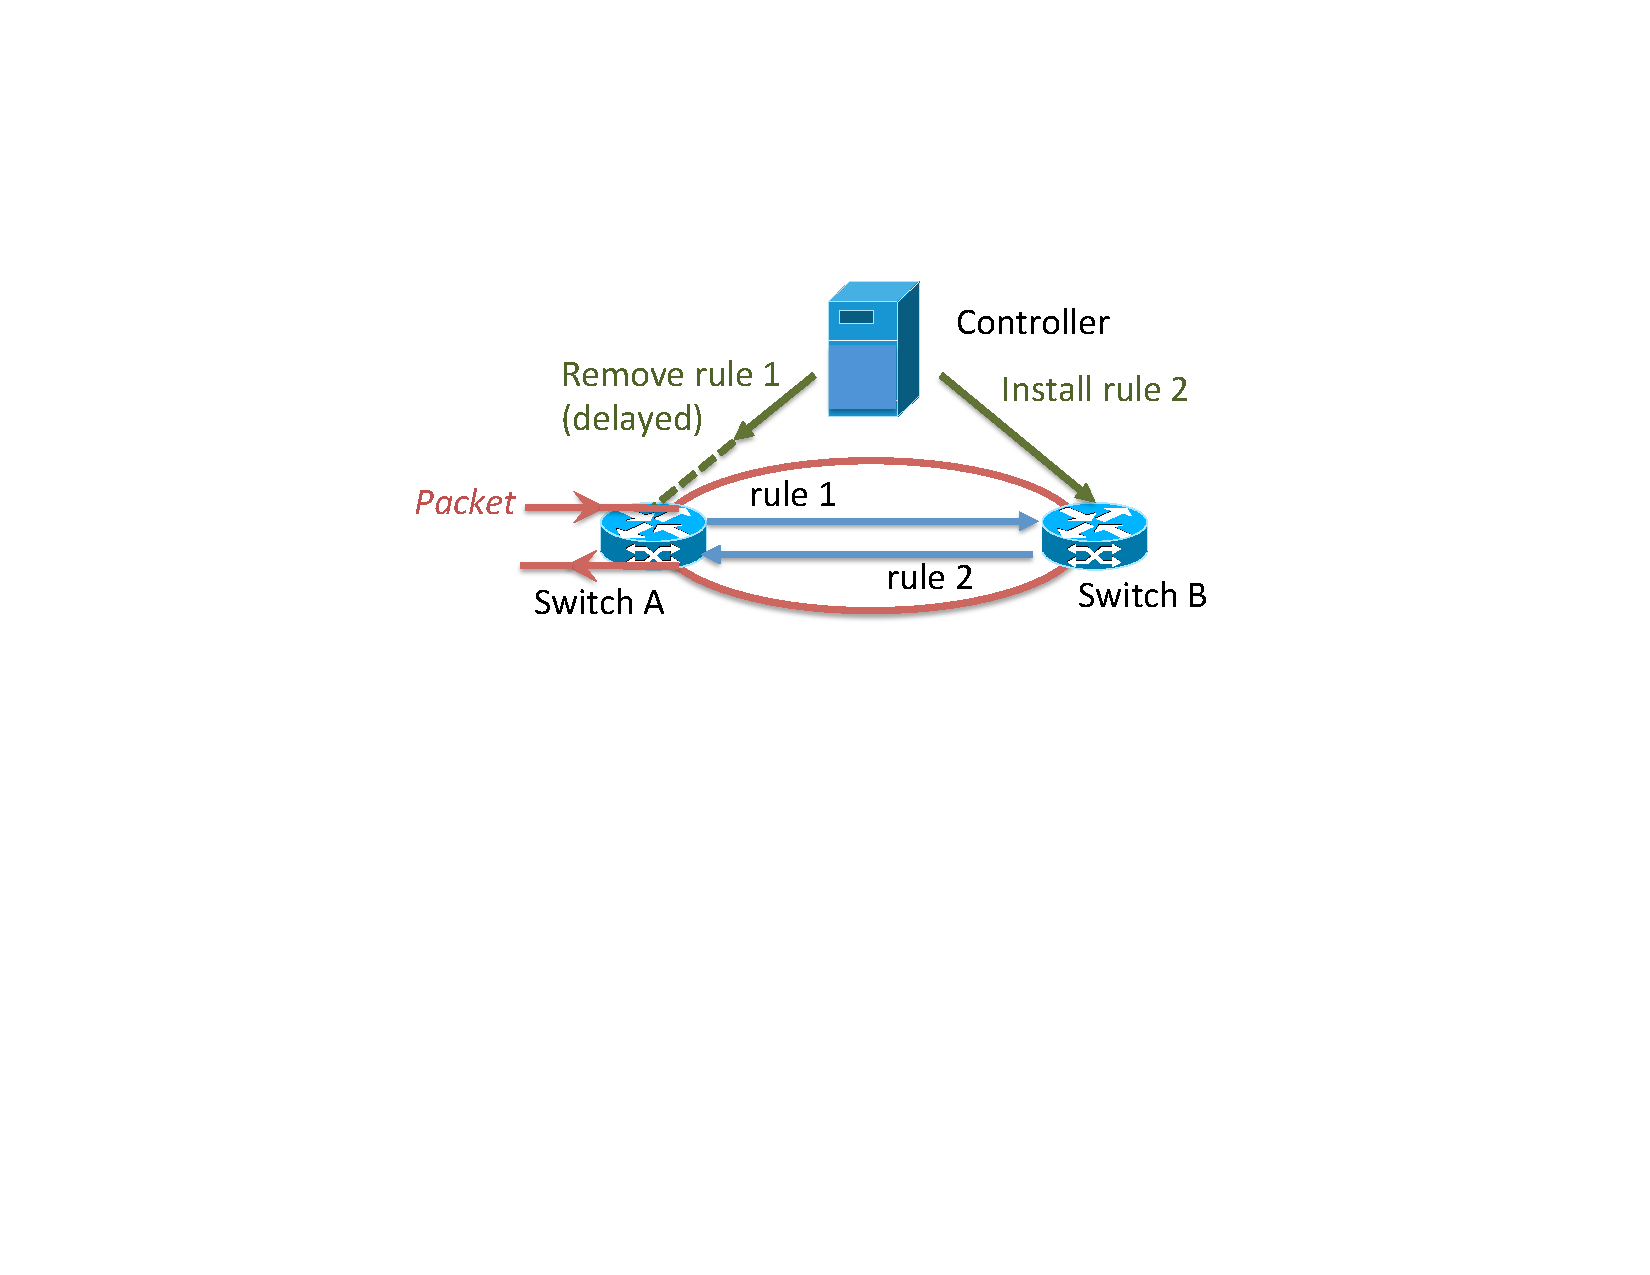
\includegraphics[width=\columnwidth]{figs/example}
%  \caption{Example.}
%  \label{fig:example}
%\end{figure}
%
%Let us look at an extremely simple example (Figure~\ref{fig:example}). Suppose there are two switches, $A$ and $B$, in the network, and switch $A$ has a forwarding rule to $B$. For the sake of simplicity, assume $A$ forwards all packets to $B$. Now the network operator wants to reverse the flow of traffic through the following two steps: 1. telling switch $A$ to remove its flow rule; 2. telling switch $B$ to insert a flow rule sending everything to $A$. Now the operator issues these two commands in this order, and neither the before or the after state of the network contains a loop between $A$ and $B$. However, we do not know when the commands arrive and are processed. It is possible that the execution on switch $B$ happens earlier than that on switch $A$, resulting a transient loop. This bug may seem not quite harmful, but the consequence of ignoring it could induce a chain of errors, especially when this transient state lasts long enough. Besides, this shows even such a simple task which is well planned in advance can go wrong due to some uncertainty. 
%%Note that in this case, serializing rule installation would help eliminate the bug, but at the cost of performance, and more importantly there are scenarios where carefully crafting ordering doesn't help~\cite{Reitblatt2012}. More devastating examples include errors caused by interleaving between packet arrivals and configuration changes, which will be discussed in more details in Section\ref{sec:motivation}.
%As for commonly used control programs, things are the same. 
%Three out of eleven bugs found by NICE~\cite{Nice2012}, (BUG-V, BUG-IX, and BUG-XI) are caused by the control programs' lack of knowledge of the network sate.  
%
%Second, such bugs may bring serious consequences.
%One may think such uncertainty related errors are all transient, and as a result, ignoring them doesn't matter much. 
%This is true with this reversing link example. 
%However, some such errors can be permanent if no attention is paid. 
%For example, if the control program asks a switch to install a rule at some point, 
%but later the program wants to withdraw this rule. 
%The problem is the two instructions can be reordered at the switch, 
%and what the switch does is first to remove a non-existing rule, 
%and then install the same rule, resulting a state against the program's intention. 
%Without querying the flow table at the switch, 
%the view of the controller and the network state will be inconsistent until the rule expires.
%One may argue that inserting a barrier message in between the two instructions solves the problem. 
%But first, this is only an example to demonstrate the point for the sake of simplicity, 
%and realistic cases are much more complex. 
%While in this case, serializing rule installation would help eliminate the bug at the cost of performance, 
%there are scenarios where carefully crafting ordering doesn't help~\cite{Reitblatt2012}. 
%Besides, it is the question who should be responsible to discover this problem and to insert the barrier message.
%As for commonly used control programs, things are the same. 
%Three out of eleven bugs found by NICE~\cite{Nice2012}, (BUG-V, BUG-IX, and BUG-XI) are caused by the control programs' lack of knowledge of the network sate.  
%
%Moreover, even if the errors disappear after a while, they have the potential to make the network suffer in terms of both security and performance. 
%%performance
%%security
%As for security, temporary access control violation may result that malicious or untrustworthy packets enter a secure zone~\cite{Reitblatt2012}. 
%%Another example is stateful firewall....
%For performance, take the previous example again. 
%If a packet enters switch $A$ while the forwarding loop exists. Note that in a realistic deployment, switches will refuse to forward packets back through their ingress port, but drop them. So the packet encounters a black hole at switch $B$ instead of a loop. A recent study~\cite{Flach2013} shows that TCP transfers with loss may take five times longer to complete compared with connections with no loss. That is, such bug may cause significant performance drop.
%%\cite{OFCPP}
%
%We conduct some measurement study to show how seriously network uncertainty can cause performance drop. Results are shown in \S~\ref{sec:bug-coverage}. 
%

%\subsection{Related Work}
%\paragraphb{Related Work.}
\if 0
\wxznew{
To rigorously check network correctness,
\cut{ software or configurations.} 
researchers have investigated various network verification techniques, such as symbolic execution~\cite{holzmann2004primer} and configuration file analysis~\cite{visser2003model, vasic2011identifying}.
\cut{
Symbolic execution
\cite{holzmann2004primer} is used to catch bugs through exploration of all possible
code paths, but is usually not tractable for large software.  Analysis of
configuration files ~\cite{visser2003model, vasic2011identifying} also helps,
but fails to find bugs in software of networking devices, and is designed
for specific configuration languages and control protocols. }
Another approach is to statically analyze snapshots of the network state 
in an off-line \cite{wang2011openflow,
heller2010elastictree, mk+sigcomm+11, cadar2008klee, baier2008principles,
flanagan2005dynamic, PHA2012} or an on-line manner
\cite{NetPlumber2013, Al-Shaer2010, VeriFlow, yang2013real}.
%. However, those previous approaches operate
%offline, and thus, find bugs only after they happen. Online verification tools
%are also developed \cite{NetPlumber2013, Al-Shaer2010, VeriFlow} to check
%dynamic snapshots in real time. 
%However, none of the existing tools take
%uncertainty caused by network dynamics into consideration.
This approach is scalable, protocol agnostic and able to catch bugs in network device software, but none of those methods consider temporal uncertainty during the transition of the snapshots. Instead, they effectively but incorrectly assume that the updates are applied at the exact moment when the verification tools see them.  
}
\fi

\if 0
Another train of inquiry \cite{incremental-cu,Reitblatt2012, zUpdate, Hong13}
focuses on how to synthesize a correct update plan to avoid inconsistencies, which may cause transient faults in the network.
Nonetheless, these solutions could be expensive in time and flow table usage and/or update delay, and they}
%However, their solutions are too expensive to achieve real-time performance
%with heavy flow table storage usage or long updates buffering time. 
%In addition, the existing approaches 
are not designed to be flexible enough to enforce generic network invariants. 
Reitblatt et al. \cite{reitblatt2013fattire} also proposed a language based on regular expressions for synthesizing
fault-tolerant network programs, but the operations have to be performed
offline.
\fi

\if 0
\kevin{Another train of inquiry focuses on how to synthesize a correct update
plan to avoid inconsistencies\cut{, which may cause transient faults in the network}.
Reitblatt et al.~\cite{Reitblatt2012} propose a two-phase update scheme to
preserve packet coherence\cut{and reachability-based invariants in SDN}.
Katta et al. \cite{incremental-cu} manage to reduce the memory requirements of
CU at the cost of longer delay. Peresini et al.~\cite{OFCPP}
propose a multi-commit transactional semantic at the controller for ensuring
consistent packet processing. Noyes et al. offer a tool to generate updates
for maintaining user-specified invariants \cite{noyes2014toward}. Researchers have
also investigated ways to preserve bandwidth-based invariants during network
transitions~\cite{zUpdate, Hong13}. The difference between our work and that earlier work is that we focus on the {\em generality} of the consistency properties that a
system needs to maintain as well as the high {\em efficiency} (fast update speed and
small memory requirement) needed to process network updates.}

Dionysus \cite{jin2014dynamic} is recently proposed to address the
efficiency issue of updating networks under general consistency requirements,
via dynamic scheduling on top of a consistency-preserving dependency graph,
which requires to be planned ahead.
%It no longer pre-determines a schedule, but still requires planning the dependency graph ahead. 
%\kevinc{I am a bit confusing about the previous sentence , (1) we already say it is dynamic scheduling, (2) we may want to say planning of what ahead, the dependency graph?} 
We take a different approach by converting complex scheduling problems to well-defined network verification problems.
\fi

%efficiency of general CU based on dynamic scheduling atop a
%consistency-preserving dependency graph. We take a different approach by
%converting the complex scheduling task into a generic verification problem.
\cut{ As discussed in ~\cite{Mahajan13}, the higher level the enforced
consistency property is, the stronger dependency is imposed among the rules,
and thus, the slower the data plane can be updated. Our black-box approach is
not only general, but also offers operators the flexibility to balance the
speed and consistency level, instead of pausing the system for strict but
unnecessary consistency enforcement. } 

\if 0
Other researchers have also noticed the problem of inconsistent view between
SDN-controller and the network states. Peresini et al.~\cite{OFCPP} proposes a
multi-commit transactional semantic at the controller for ensuring consistent
packet processing. Heller et al.~\cite{sdnlayering} presents a big picture of
cross-layer diagnostic framework for systematic troubleshooting in SDNs, and
rigorous network-wide verification which we have explored in this paper, is an
essential component towards that goal. 
\fi
%4. Stateful firewall (logic programming for SDN)	
%
%The key idea: the domain is able to send any traffic to the outside world, while an outside entity is only allowed to send traffic into the domain if the domain has first sent it a packet. 
%
%Model: one switch with two ports. Port 1: the external world, port 2 internal.
%Any pkt that arrives on port 2 is routed to port 1. In addition, the firewall remembers the dst IP of such a packet. 
%Any packet that arrives on port 1 is dropped unless the src IP matches one of the IPs that it has remembered. In this latter case, it forwards the pkt to port2.
%
%
%Default rule: any traffic that comes in on port 2 to be forwarded out on port 1
%Each pkt with a unique dst IP arriving at port 2 should be sent to the controller. When such a packet is processed, the run-time system extracts the dst IP and stores it as seen, and generates a specific rule that all traffic appearing on port 1 whose srcip field is IP is forwarded out port 2.
%
%Events: 1. client sends a pkt to server
%
%	2. SW sends this pkt to Controller
%
%3. Controller sees the pkt, stores dst ip IP, installs a rule that allows pkt whose srcip == IP from port1 to port2
%
%In VF: 	Init: 	for EC (c-->s) c-->SW-->s
%
%for EC (s-->c) c     SW<--s 
%
%after event 3, for EC (c-->s) c-->SW-->s
%
%for EC (s-->c) c<--SW<--s 
%
%But in reality, rule could arrive at SW after server’s response
%
%then for this pkt, EC(s->c) still c  SW<--s
%
%could be detected by VF with uncertainty


%\section{Maximizing Parallelism}

%\section{Customizable Consistency Constructor (\name)}
\section{Customizable Consistency Generator}
\label{sec:overview}

%\wxzc{ 
%Outline:
%
%1. the problem can be reduced to a verification problem. why? Questions: 1) uncertainty->a number of simultanenous possible views; 2) a number of possible sequence updates;
%
%2. to Q1, existing verifiers don't consider uncertainty, effectly assume ...;
%
%3. to Q2, heuristic..., fallback ...;
%
%4. Figure 1
%}

%\wxzc{what: General consistency properties

%how: our system is designed as a wrapper around a verificaiton engine -- the verificaiton engine can take as input arbitrary invariants -- since we treat the VE as a black box, we can use it to implement arbitrary consitency properites}
%
%Ultimate goal: handle generilized consistency properties efficintly
%
%Approach: uncertainty-aware modelling, black-box verification, synthesis algorithm
%
%In this section, we provide an overview of our system, \name.
%
%Workflow:
%
%Step1: verification
%
%Step2: enforce correctness, algorithm
%
%\label{sec:structure}

\name works by converting the update scheduling problem into a network verification problem, in which arrows indicate flows of network messages (updates or acknowledges).  
%To efficiently enforce consistency of network-wide invariants and policies as
%network states evolve, we convert the complex update scheduling problem into a
%well-defined network verification problem. 
Our overall approach is shown in Figure~\ref{fig:structure}.
Our uncertainty-aware network model (\S\ref{sec:model}) provides a compact symbolic
representation of the different possible states the network could be in,
providing input for the verification engine.
%models the inputs for the verification engine
%Figure~\ref{fig:structure} depicts the system architecture
%Our
%uncertainty-aware network model produces inputs for the verification engine, in
%a manner that accurately captures the network uncertainty (\S\ref{sec:design}). 
The verification engine is responsible for verifying 
application updates against {\em any} specified
invariants and policies (\S\ref{sec:verify}). 
Based on verification results, \name synthesizes an
efficient update plan to preserve policy consistency during network updates,
using the basic heuristic and a more heavyweight fallback mechanism as backup 
(\S\ref{sec:parallelism} and \S\ref{sec:synthesis}).  
One key feature of \name is that it operates in a {\em black-box} fashion, providing
a general platform with a very flexible notion of consistency.
For example, one can 
%One key feature of \name is that as a platform, it
%operates in a black-box fashion, offering a very flexible notion of
%consistency. Therefore, one can 
``plug in" a different verification
function and an update scheduling tool to meet one's customized needs.
%A key feature of \name is that it runs both the verification engine and
%the fallback mechanism in a black-box fashion.  That is, one can plug in
%different checking functions and update tools to leverage the flexible support
%for invariant checking that our general network model provides, and the
%consistency properties those update tools guarantee, respectively.

\begin{figure}[!ht]
  \centering
  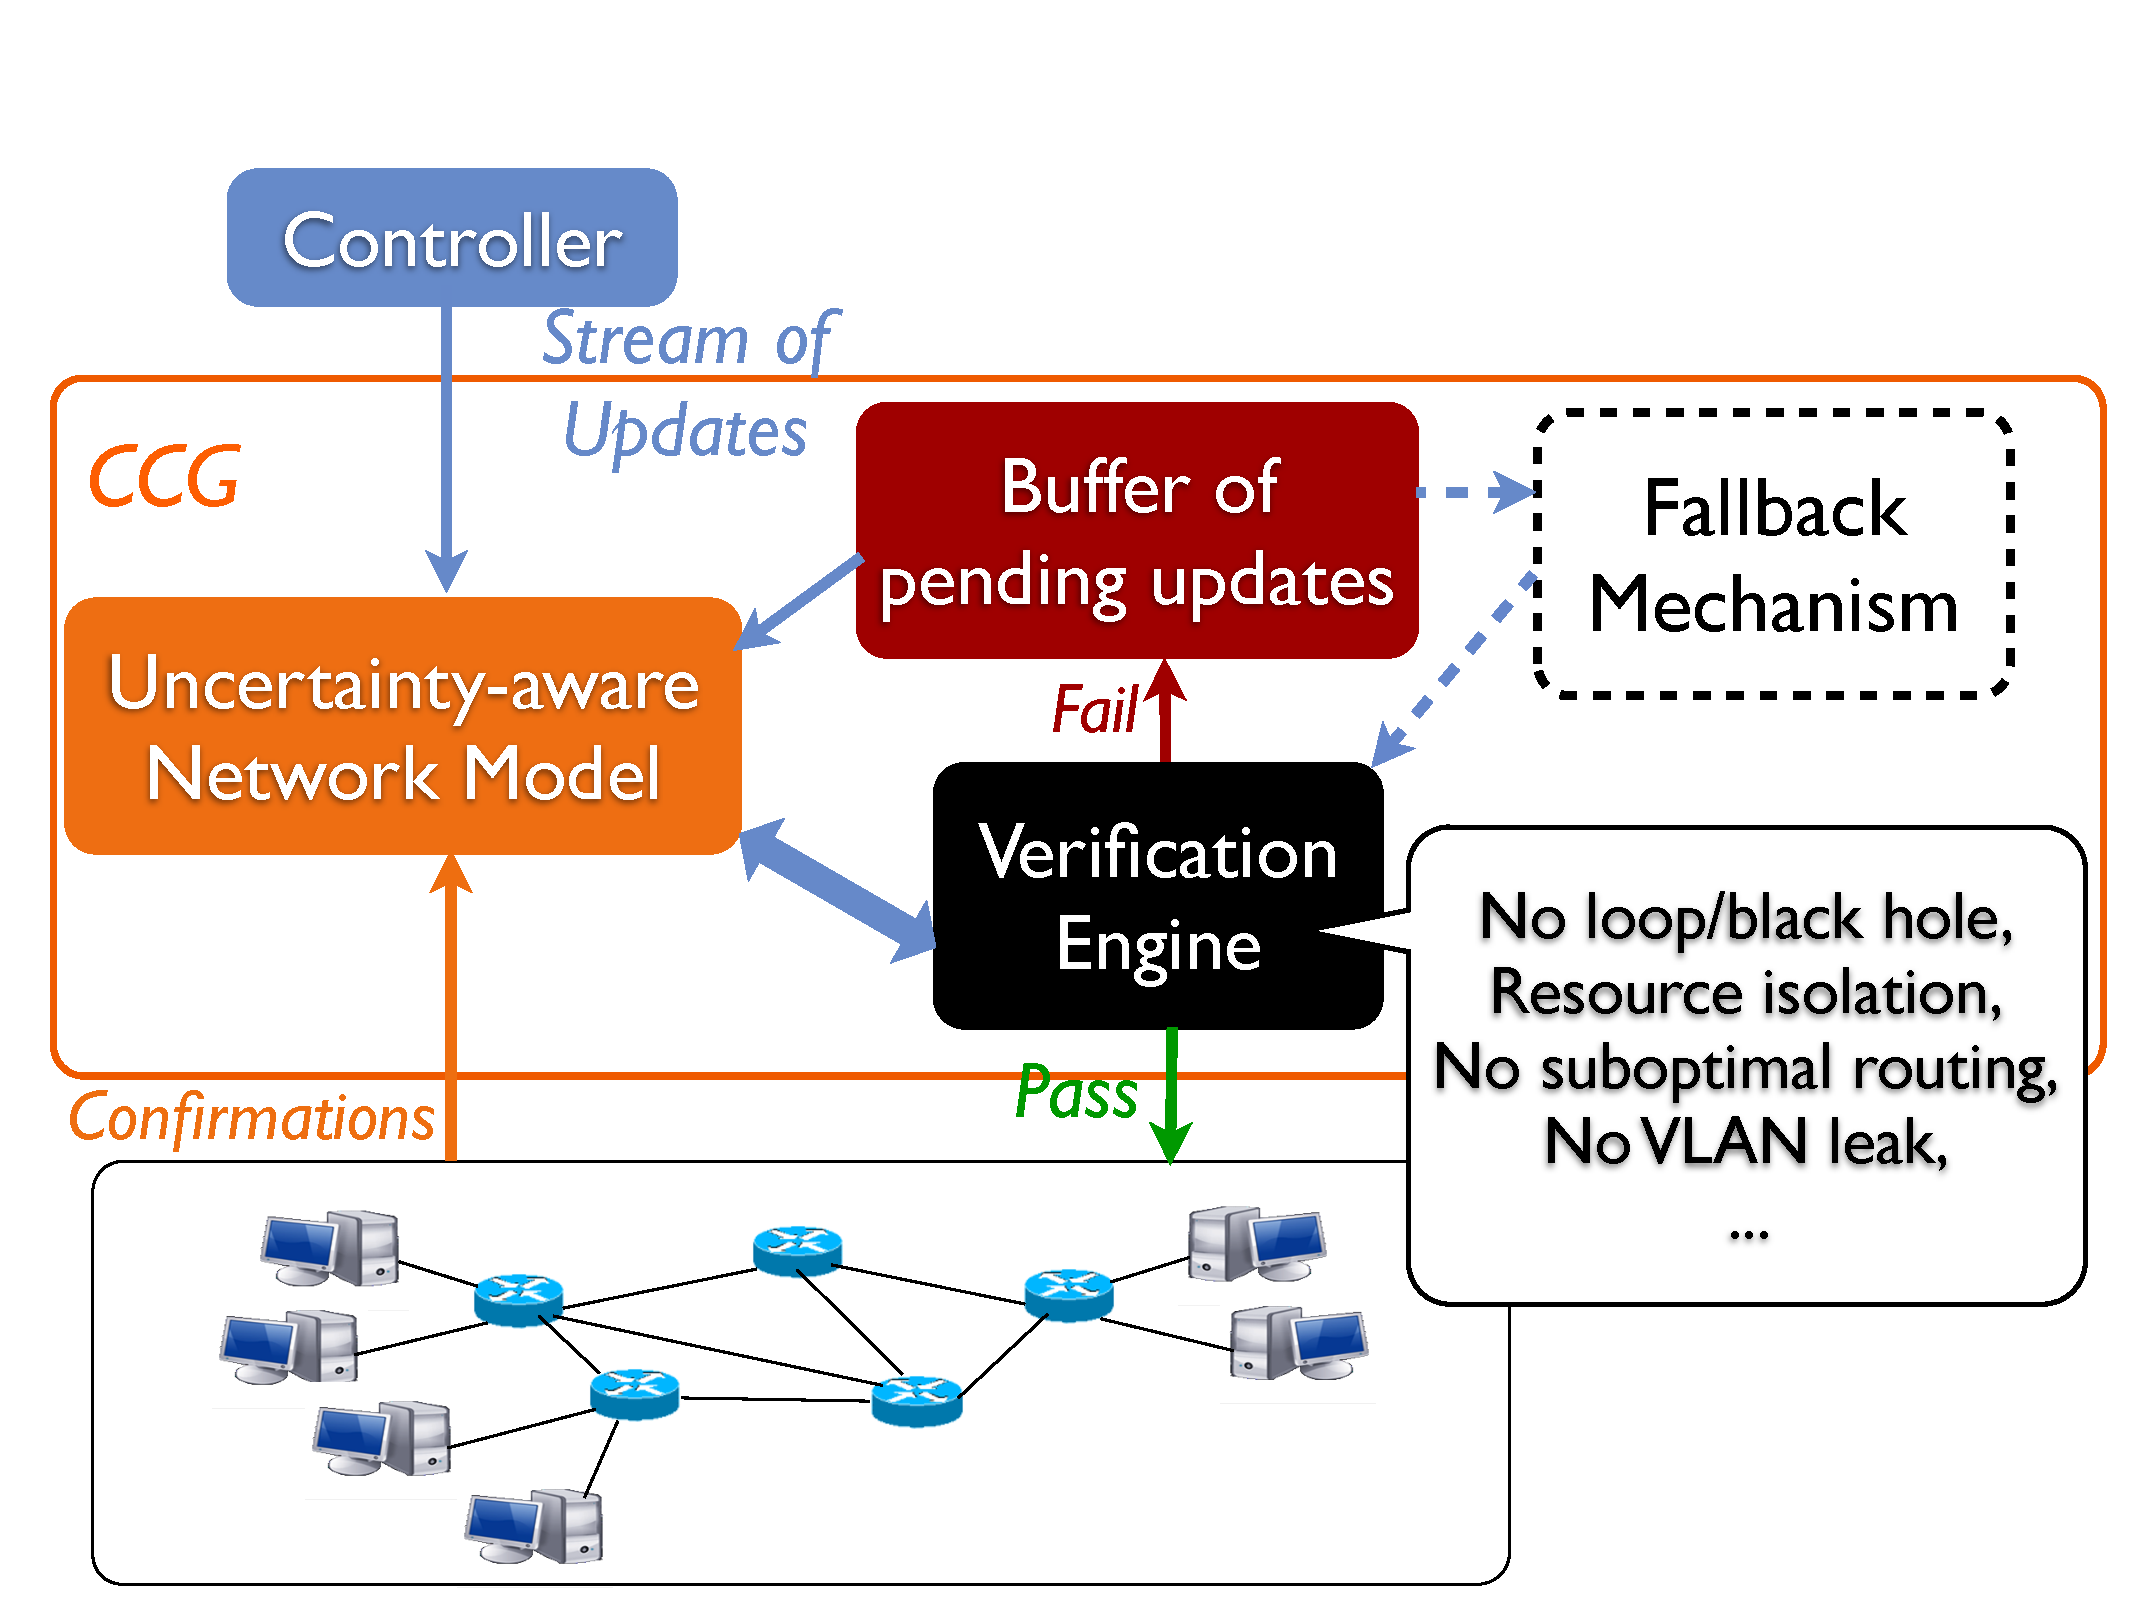
\includegraphics[scale=0.2,trim=0 0 0 1cm]{figs/structure_new}
  \vspace{-0.1in}
  \caption{\em \small System architecture of \name.}
  \vspace{-0.2in}
  \label{fig:structure}
\end{figure}

%  \if 0
%As discussed in \S~\ref{sec:motivation}, guaranteeing generalized consistency properties with maximized efficiency is important, yet difficult.  
%  \cut{
%  Achieving stronger consistency properties may require slowing of the process of updating
%  the data plane, thus harming convergence time and reaction speed.  To achieve a good
%  tradeoff between consistency and efficiency, recent work~\cite{Mahajan13}
%  proposed a scheme to maximize update speed in the context of preserving loop
%  freedom. However, that approach, while useful, provides an algorithm tailored to achieve just a single goal, loop freedom, instead of supporting general
%  consistency properties.  In contrast, our work aims to provide a flexible framework.}
%allowing custom specification of consistency properties, and an algorithmic approach
%to enforce them with good efficiency.


 %and is hence not capable of supporting general consistency properties. In contrast, our work aims to develop a {\em general} framework, which 
%supports a more arbitrary set of consistency properties to be 
%
%The stricter the desired consistency property is,
%%(e.g., packet coherence is a stricter requirement than loop freedom), 
%the slower the data plane can be updated to preserve it.
%To achieve a better consistency-efficiency tradeoff, specific mechanisms that guarantee specific properties
%are proposed. For example, an algorithm tailored for the property of loop freedom is designed to achieve minimal dependency among rules, and thus maximized update speed under the property~\cite{Mahajan13}.
%Such specified tool is useful, but not capable of supporting general consistency properties.
%Thus, a general framework that supports customized property is desired. 
  \if 0
%\wxznew{
%  The problem of enforcing generalized consistency with\cut{ maximized} \wxznew{high} efficiency, 
%  we show, can be reduced to a general verification problem.
%  In particular, the problem of determining a schedule of 
%  when to send updates can be reduced to checking, 
%  with a network verification tool, whether the
%  schedule produces a network that obeys a provided set of consistency invariants.
%  
%  However, checking every possible update ordering would be really
%  inefficient. What's more, even at a single time point, due to the inherent ``network uncertainty" (defined later in \S\ref{sec:design}),
%  one has to check all possible views of the network at that moment to rule out any possiblity of violating policies.
%  \fi

\kevin{
To efficiently enforce general consistency properties on network-wide state,
we convert the update scheduling problem into a network verification problem.
One way to do this would be to enumerate all possible update orderings, and run a
network verification tool~\cite{VeriFlow, NetPlumber2013} after each update, for each possible ordering.
If the network verifier fails on an update, we reject the sequence.

However, this approach would not be very efficient, as the number of possible update orderings
can be large, growing exponentially with the number of queued updates.
 %verifying every possible update ordering would be very inefficient. 
Moreover, this space may be even larger---even at a single instant in time, 
the inherent ``uncertainty" the controller has in the
current state of the network complicates things further. For example,
if the controller recently sent an update, but has not yet received an
acknowledgment, the controller may not be sure what state the network
is currently in. Based on the knowledge it does have the controller
may be able to enumerate the set of possible states the network may be
in, but it must check all of these possible states to rule out the
possibility of violating the consistency policies. This number of states can again
be large (increasing exponentially with the number of unknown forwarding table entries,
for example), and hence such an approach would not be efficient.
%Moreover, at any instance of time, due to the inherent ``network uncertainty" (defined in \S\ref{sec:design}), one has to check all possible views of the network to eliminate any possible policy violations.
}
%Because
%of the distributed nature of networks, the \name engine is unaware of the precise ordering and timing with which updates arrive at devices in the network. To address that, \name explicitly models the “uncertainty” about network state through the use of a novel symbolic network repre- sentation, a data structure that compactly represents all different possible network states.

%in the sense that a
%general network verifier would be able to determine whether any update is safe to pass
%to the network at any time.  
%Using that information, we could greedily
%proceed with network state transition, and heuristically achieve maximized update
%parallelism.

On top of all this, we
%Because of these challenges, we
cannot utilize existing network verifiers, such as VeriFlow~\cite{VeriFlow} and~\cite{PHA2012}
, which inaccurately assume 
%To deal with the \cut{multiple }simultaneous possible network views, \cut{unfortunately, }we cannot utilize 
%existing network verifiers, such as VeriFlow~\cite{VeriFlow} or HSA~\cite{PHA2012}, 
%which effectively yet inaccurately assume 
that updates are applied
at the exact moment when the verification tools see them.
Tools such as VeriFlow and HSA only check
static network snapshots, and do not consider temporal uncertainty
during the transition between snapshots, which can lead to false
positives and false negatives in their diagnoses in practical
settings.
%In other words, they only check static network snapshots, and do not consider
%causing these network models to be inaccurate to some extent.
%temporal uncertainty during the transition of the snapshots.

To deal with these challenges,
\name explicitly models the {\em uncertainty} about network state 
with a novel symbolic network representation --- a data structure that compactly represents all different possible network states. 
%\wxzc{same text as in intro now, need to be changed later.}
%compactly storing the diffiernet options using your symbolic network
%representation and traversing it. 

However, another challenge remains. How can we efficiently find a feasible update sequence that preserves
the desired policies among all possible sequences?
%\cut{while updating the network efficiently. For efficiency purpose, }
To address this, \name uses a greedy heuristic algorithm.
The algorithm utilizes the network verifier to determine whether an update is safe to pass to the network at a given time, if it is it passes it to the network, if not it buffers it.
Upon receiving new information (new updates, acknowledgments from network), it re-checks and attempts to re-send buffered updates.
Our heuristic attempts to maximize parallelism, by automatically determining which update groups could ``conflict'' in the network (in the presence of uncertainty). 
%\kevin{The algorithm utilizes the network verifier to determine whether an update is safe to pass to the network at a given time; it then greedily processes the network state transition, and heuristically maximizes the parallelism of updating the network. 
We formally identify the large scope of consistency policies that are guaranteed by \name's heuristic (\S\ref{sec:seg-independence}). \name achieves high update efficiency (in both speed and memory consumption) by attempting to handle updates with the heuristic, and falling back to other heavyweight techniques (e.g., CU~\cite{Reitblatt2012} and SWAN~\cite{Hong13}) only when necessary (very rare in practice as shown in \S\ref{sec:eval}) to guarantee the provided
set of consistency policies. 

%Figure~\ref{fig:structure} depicts the system architecture. One key feature of \name is that as a platform, it operates in a black-box fashion, offering a very flexible notion of consistency. 
%Therefore, operators can ``plugin" a different verification engine and an update scheduling tool to meet different needs.
}

% \if 0
% as a general network verifier would be able to determine whether any update is safe to pass
% to the network at any time. Using that information, the algorithm 
% greedily proceeds with network state transition, 
% and achieves heuristically maximized update parallelism.
% We formally identify the scope of consistency policies 
% (actually covering a fairly large set of policies) that are guaranteed by 
% \name's heuristic (\S\ref{sec:seg-independence}), and experimentally 
% show its ability to achieve high update efficiency (\S\ref{sec:seg-independence}).
% \name also employs relatively more heavyweight update tools,
% such as CU~\cite{Reitblatt2012} and SWAN~\cite{Hong13},
% as plug-ins. Those plug-ins are triggered only when the heuristic can not find a feasible sequence 
% (very rare as showed in \S\ref{sec:eval}), to ensure supplied consistency policies.
% 
% 
% Figure~\ref{fig:structure} depicts the system architecture. 
% Our uncertainty-aware network model produces inputs for the verification engine, in a
% manner that accurately captures the network uncertainty.
% The verification is responsible for verifying application updates against {\em any} specified invariants and policies.  
% Based on verification results, \name synthesizes an efficient update plan to 
% preserve policy consistency during network updates,
% using the basic heuristic and a more heavyweight fallback mechanism as back up. 
% A key feature of \name is that it runs both the verification engine 
% and the fallback mechanism in a black-box fashion. 
% That is, one can plug in different checking functions and update tools to
% %Doing so enables \name to 
% leverage the flexible support for invariant checking that our general network
% model provides, and the consistency properties those update tools guarantee, respectively.
% \fi
%}

% \if 0
% However, two key challenges remain. First, existing network verification tools, such as 
% %In order to enforce general consistency properties, \name is designed as a wrapper around a \matt{{\em verification engine}, such as 
% VeriFlow~\cite{VeriFlow} and HSA~\cite{PHA2012}, only check static network snapshots against desired properties, and do not consider
% the dynamics inherent in the network.  
% Second, a greedy algorithm such as the one we describe above could get stuck,
% % \mattc{todo:how?}, 
% and then either the whole system would be paused, or
% the \cut{specified} desired consistency properties would be violated.
% 
% %\wxz{Note that there are scenarios where no combination of updates ordering can support the required policy~\cite{Reitblatt2012}. That is, some buffered updates could never be safe to pass to the network.
% To address the first challenge, we designed a network modeling technique that is aware of dynamic settings of the network (\S\ref{sec:design}).
% %Specifically, taking into account the controller's inherent uncertainty about the current state of the network, 
% %\name maintains an {\em uncertainty-aware network model}. 
% That network model \cut{is used to }produces inputs for the verification engine, in a
% manner that accurately captures \wxznew{the dynamics}.%this uncertainty.
% \fi
\if 0
\wxznew{
Due to the second challenge, we adopt a hybrid approach for the design, depending
on the consistency requirement.
As we will show in \S\ref{sec:seg-independence} and \S\ref{sec:eval}, there are
a group of consistency policies, which covers a fairly large set of common policies,
can be guaranteed by the greedy heuristic of \name. 
Hence in this case, we expose the verification engine to application directly, 
ensuring the desired policies while introducing zero extra overhead.
As for policies fall out of this group, thanks to existing update mechanisms,
some of them can be guaranteed if the operators are willing to suffer additional storage
or time overhead. 
Under such circumstances, a layer between the controller applications 
and \name, translation layer, is triggered. 
%In that case, we can adopt two possible alternatives. 
%One is to insert a layer of existing update mechanism, like that proposed in Reitblatt et al.~\cite{Reitblatt2012}, which guarantees the required policy.% between control applications and \name. 
The stream of updates from the application is first fed into 
the translation layer to be transformed to a feasible update sequence. 
Then \name greedily sends updates as long as the policy is preserved. 
In this way, \name is guaranteed to preserve
%correctness is maintained all the time at the cost of extra control overhead and device memory. In other words, \name is able to maintain 
the same level of consistency as the mechanism used in the inserted layer.
This approach suffers an added cost of adding an amount of control and device
memory overhead equivalent to that if using that mechanism separately, but
retains the advantage of greatly shortened the update delay.  Because of the
shorter delay, the period of time that network suffers from heavy memory
overhead is reduced.  
Alternatively, if the operators value update efficiency, and only ask for best-effort to 
maintain consistency during updates, the translation layer won't be triggered, 
but instead, after a configurable threshold, buffered commands are released to the network (\S\ref{sec:parallelism}).
That is, operators have a choice of balancing efficiency and consistency trade-off.
%However, maintaining properties does not necessarily
%require use of such a layer, as we later show in \S\ref{sec:eval}.
}
%However, there are properties, assurance of which don't require such a heavy layer, as we show~\ref{sec:eval}.
%Hence another alternative is to expose the verification engine to application directly, which reduces control and device memory overhead further.
%, sacrifice correctness to some extent but maintains high efficiency. For example, to limit disruption on network operations, the network operator can specify a timeout value, upon on the expiration of which a buffered update is issued.}
\wxzc{Change to one approach. Fall-back mechanism: issue the buffered updates
after a threshold of waiting time use 2-phase update.}

\kevin{
To address the second challenge, we began by formally identifying the scope of consistency policies 
(actually covering a fairly large set of policies) that are guaranteed by 
\name's heuristic (\S\ref{sec:seg-independence}).
%never get stuck with \name's greedy heuristic. 
\cut{The performance is extremely fast because of the direct interaction between the verification engine and the applications. }
For policies outside that scope, our approach is to integrate \name's
heuristic with existing update mechanisms in the following way. Upon
receiving network updates from applications, \name greedily sends updates as
long as the desired policy is preserved. Whenever \name gets stuck on an
update, it automatically falls back to other consistent update tools, such as
CU~\cite{Reitblatt2012} and SWAN~\cite{Hong13}. 
Thus, our algorithm guarantees the same level of
consistency as the existing solutions do. 
\cut{The hybrid approach is slower than \name, but not surprisingly so; it still greatly shortens the update delay and
reduces the memory overhead, compared to CU~\cite{Reitblatt2012} and SWAN~\cite{Hong13} used alone.} 
%Alternatively, if the operators value update efficiency, and only ask for best-effort to 
In fact, in many cases, network operators value updates efficiency (e.g., speed), 
and only ask for the best-effort to maintain consistency.
%without losing too much efficiency during network updates. 
Then \name is able to offer the flexibility to balance between efficiency and consistency
through a configurable timing threshold, over which buffered commands are simply
released to the network.}
\fi

\if 0
\name consists of the following components, as shown in
Figure~\ref{fig:structure}: an uncertainty-aware network
model\cut{(\S\ref{sec:design})}, a translation layer, a black-box verification
engine, and a data structure that buffers problematic updates temporarily. 
%The translation layer produ \mattc{missing text?}
The verification engine leverages the network model, and is responsible to
verify updates against {\em any} specified invariants.  Based on verification
results, \name provides an algorithm to synthesize a correct and efficient update plan,
\wxznew{with the help of the translation layer when necessary}.
\fi

%for when, where, and how to release buffered updates to the network
%(\S\ref{sec:parallelism}).

%Doing so enables \name to make direct use of these tools' capabilities of checking (but not instilling) correctness properties.}

%Second, it is difficulty to support an \emph{arbitrary}\wxzc{should we say "arbitrary" or be a little conservative here?} consistency property.
%If the policy verification function is tightly coupled with other components, 
%whenever a different policy is desired, we end up redesign the entire system. 
%To this end, we design a platform, which takes the decision procedure of 
%any property of interest as a plug-in module 
%rather than reasoning a specific property invariant.
%We name this plug-in module as black-box verification engine.
%Given an update and a network model as inputs, 
%a black-box engine simply outputs whether or not this update passes the specific verification.
%%For any given consistency requirement, for example, two hosts c , or no suboptimal routes, 
%%is specified as a verification engine plugged into the framework. 
%Based on the outputs, we design an algorithm to synthesize an update plan 
%compliant with the property while maximizing update parallelism.
%In this way, we are able to realize flexible network consistency notion.
%%without any knowledge of internal workings of the verification engine.
%\paragraph{Uncertainty-aware network model}

%\paragraph{Black-box verification engine}
%\if 0
%A key property of \name is to run the verification engine in a black-box fashion.
%Doing this enables \name to leverage the flexible support for invariant checking
%that existing network verifiers already provide.
%\name assumes the verification engine operates in a per-update fashion (a la Veriflow, NetPlumber, and FlowChecker~\ref{Al-Shaer2010}). \wxz{For each update, it takes the update as well as a graph representing network states, such as our network model(\S~\ref{sec:design}) as inputs}, and outputs a {\em pass} if the update does not violate invariants, and a {\em fail} otherwise.
%\mattc{Wait a second... you don't really use the verifier as a black box right? You need to feed that symbolic graph into it. Don't you need to extend the verifier to deal with symbolic links? If so you need to describe that briefly here, and maybe tone down "black box".}
%\name then uses this output to synthesize an update ordering that obeys the provided set of correctness
%invariants.
%To do this, \name retains a buffer of updates -- if an update fails the verification process,
%it can be buffered until a point where the update becomes safe to send. \mattc{what if this never happens? do you eventually discard? where do you discuss this in the paper?}
%\mattc{I didn't understand a lot of the paragraph that was here so I cut it -- is what I wrote above missing anything you wanted to say? your paragraph is commented out here:}
%\if
% Inspired by black-box testing techniques, the verification functionality in \name is designed as a black-box \matt{unit within} our network model\mattc{I don't see how it's inspired by that in particular}.
% \name takes the decision procedure of any properties of interest as a plug-in module rather than reasoning a specific property invariant\mattc{I can't parse this sentence, what does it mean?}.
% We name that plug-in module as black-box verification engine.
% %If the policy verification function is tightly coupled with other components, 
% %whenever a different policy is desired, we end up redesign the entire system. 
% The design goal is to support arbitrary invariants. Once a invariant or a set of invariants is specified, a corresponding verification engine is plugged into \name. The verification engine takes the network model and network updates as inputs, and examines whether applying the updates to the model could violate the invariants. 
% That is, we do not need to peer into its internal structures and workings, 
% or modify any other modules of \name.
% In addition, programmers can write their own checkers with the unified interfaces.
% For each update, the verification engine simply outputs whether or not the update violate any invariant.

%The outputs of the verification engine are 
%(1) whether or not the update violates the invariant(s), and 
%(2) all the possible locations where that update fails the verification, i.e., the possibility of safely issuing that update later relies on the status of some future or in-flight updates on those locations.
%Note that it is the invariant that determines the dependencies among updates.
%Note that such dependencies vary as invariants change.
%Take Figure~\ref{fig:dependency} as an example...
%
%loop
%
%black hole

%\paragraph{Dependency graph buffer}
%We develop a graph type data structure to temporarily store updates that don't pass the verification. The reason that a graph is used here, is to present the dependency between updates. As stated above, invariants determine the dependency relationships among updates, 
%and the verification engine outputs such relationships to the dependency graph.
%From any location that a buffered update is relying on to this update there is a directed link. Any future change on one of the locations will activate reprocessing of this update, 
%to see if it's the time to pass it to the network. More details are in \S~\ref{sec:algo}. 
\fi


%\section{Uncertainty-aware Network Modeling}
\section{Verification under Uncertainty}
\label{sec:design}

%\wxzc{ to examine consistency during network updates;}

\kevin{We start by describing the problem of network uncertainty (\S\ref{sec:uncertainty}), and then present our solution to model a network in the presence of uncertainty (\S\ref{sec:model} and \S\ref{sec:confirm}).} Our design centers around the idea of \emph{uncertain forwarding graphs}, which compactly represent the entire set of possible network states from the standpoint of packets.
\wxzcr{Next, we describe how we use our model to perform
uncertainty-aware network verification (\S\ref{sec:verify}).}
%\mattc{add a one-sentence roadmap giving the flow of this section}
%We start by introducing the problem of network uncertainty (\S\ref{sec:uncertainty}). We then present \name's uncertainty-aware network model (\S\ref{sec:model} and \S\ref{sec:confirm}).

%, and how to perform network-wide verification using this model (\S\ref{sec:verify}).
%In this section, we describe our design of modeling network state taking uncertainty into account. 

%First, we slice all packets that may enter the network into \emph{equivalence classes} (ECs).
%Each EC is a set of packets that experience the same forwarding actions throughout the network.
%More formally, an EC is defined as:

%\wxzc{Equivalence Class definition, borrowed from veriflow}
%In order to confine our verification activities to only the affected set of packets,
%we slice the network into a set of equivalence classes (ECs) based on the new rule and
%the existing rules that overlap with the new rule. 
%\paragraphb{Definition (Equivalence Class): } An equivalence class (EC) is a set $P$ of packets such that-
%for any $p_1, p_2\in P$ and any network device $R$, the action is identical for $p_1$ and $p_2$ at $R$.

%Next, we model the behavior of packets% belonging to each EC 
%as a graph. 
%Such graphs changes as network states modifications, such as rule additions, removals, or physical failures, happen.
%What is challenging is that from network control point of view, how to model the uncertainty during state transistions?
%Typically, a set of rules in data plane that affect a particular EC is a subset of the entire rule set.
%Similarly, any rule only influence a limited number of ECs in most cases.

%move to implementation
%\subsection{VeriFlow}
%\label{sec:veriflow}
%As the foundation of our work, we first briefly introduce VeriFlow, a real-time network-wide verifier.
%Sitting between the controller and the network, VeriFlow intercept every update issued by the controller before it hits the network and verify its effect in real-time through the following three steps.

%First, VeriFlow slices the entire packet space into a set of Equivalence Classes (ECs) of packets
%using all existing forwarding rules and the new update.
%Each of the ECs is a set of packets that experience the same forwarding actions throughout the network.
%Because each update typically affects a very small number of ECs, 
%to limit searching space,
%VeriFlow only focuses on ECs that might be influenced by the new update. 
%Second, VeriFlow builds a forwarding graphs for each of the affected ECs respectively, 
%representing forwarding behaviors of packets belonging to those ECes.
%Last, VeriFlow traverses each of these graphs,
%to verify network-wide invariants.

\subsection{The Network Uncertainty Problem}
\label{sec:uncertainty}

%We first describe the problem of network uncertainty and the negative effects of neglecting it.
% on network-wide verification. 
\pbg{Networks must disseminate state} among distributed and asynchronous devices,
which leads to the inherent \emph{uncertainty} that an observation point
%\cut{tasked with instilling updates consistently into the network, e.g., }
has in knowing the current state of the network. %\kevinc{I prefer to remove the sentence ``which leads to ... by the network".}
We refer to the time period during which the view of the network from an observation point (e.g., an SDN controller)
might be inconsistent with the actual network state as {\em temporal network uncertainty}.
%\mattc{I don't get this sentence -- are you defining "temporal network uncertainty" as a term? If so make it italic and say "Let us refer to the". Or are you defining a quantity here?}. 
The uncertainty could cause network behaviors to deviate from the desired invariants 
temporarily or even permanently. 
%This deviation can affect network verification negatively because of the following two reasons.

%In this section, 
%Here, we define the inconsistency between the view of the observation point and the network state data packets encounter as network uncertainty.

%Network temporal uncertainty imposes a question to network verification: \emph{What if there is uncertainty of the presentation of the network snapshots?}. More specifically, in this paper, we focus on data plane verification by analyzing snapshots of the network-wide data-plane states~\cite{Al-Shaer2009, Al-Shaer2010, VeriFlow, PHA2012, NetPlumber2013}. Before answering this question, we first illustrate how serious the uncertainty can affect network verification.

%First, the bugs caused by such uncertainty, and thus neglected by the current data-plane verifiers, are prevalent.\mattc{I don't see how this paragraph shows they are prevalent. You don't give any statistics about how common they are. Maybe change this into just a motivating example?}
%To illustrate how uncertainty makes the problem much harder,
\if 0
As a motivating example (Figure~\ref{fig:example}), suppose there are two
switches, $A$ and $B$, in the network, and switch $A$ has a forwarding rule
\matt{directing traffic} to switch $B$. 
%\cut{
%For the sake of simplicity,
%\matt{assume this rule causes $A$ to} forward all packets to $B$. 
%}
Now the
network operator wants to reverse the flow of traffic, by making, in sequence,
the following two changes to the network: (1) make switch $A$ remove its
forwarding rule; (2) make switch $B$ insert a new forwarding rule which sends
all traffic to $A$. The network does not contain a loop between $A$ and $B$
before nor after the commands are issued.
However, we do not know exactly when the commands arrive and are processed by
the switches. It is possible that the operation on switch $B$
happens earlier than the one on switch $A$, which results in a transient
loop, leading to increased traffic load as well as lost packets.
%\mattc{I didn't understand the text that was here on "chain of errors" -- how could it cause a chain of errors? What do you mean by chain of errors?}
% the consequence of ignoring such bugs could induce a chain of errors, especially when the transient state lasts sufficiently long. Besides, the example shows that even such a simple and well-planned task can go wrong due to network temporal uncertainty. 
% %Note that in this case, serializing rule installation would help eliminate the bug, but at the cost of performance, and more importantly there are scenarios where carefully crafting ordering doesn't help~\cite{Reitblatt2012}. More devastating examples include errors caused by interleaving between packet arrivals and configuration changes, which will be discussed in more details in Section\ref{sec:motivation}.
% Similar errors can happen in commonly used control programs too. For 
This is not an uncommon--three out of eleven bugs found by NICE~\cite{Nice2012}, 
(BUG V, IX, and XI) are caused by the control programs' lack of knowledge of the network states.

the following two changes to the network: (1) make switch $A$ remove its
forwarding rule; (2) make switch $B$ insert a new forwarding rule which sends
all traffic to $A$.
\fi

\kevin{
Figure~\ref{fig:mt_example} shows a motivating example. Initially, switch $A$ has a forwarding rule
directing traffic to switch $B$. Now the operator wants to reverse the traffic by issuing two instructions in sequence: (1) remove the rule on $A$, 
and (2) insert a new rule (directing traffic to $A$) on $B$. 
%Because of the network uncertainty, 
But it is possible that the second operation finishes earlier than the first one, 
causing a transient loop that leads to packet losses.
That is not an uncommon situation; for example, three out of eleven bugs found by NICE~\cite{Nice2012} 
(BUG V, IX and XI) are caused by the control programs' lack of knowledge of the network states.
}

\begin{figure}[!ht]
  \vspace{-0.1in}
  \centering
  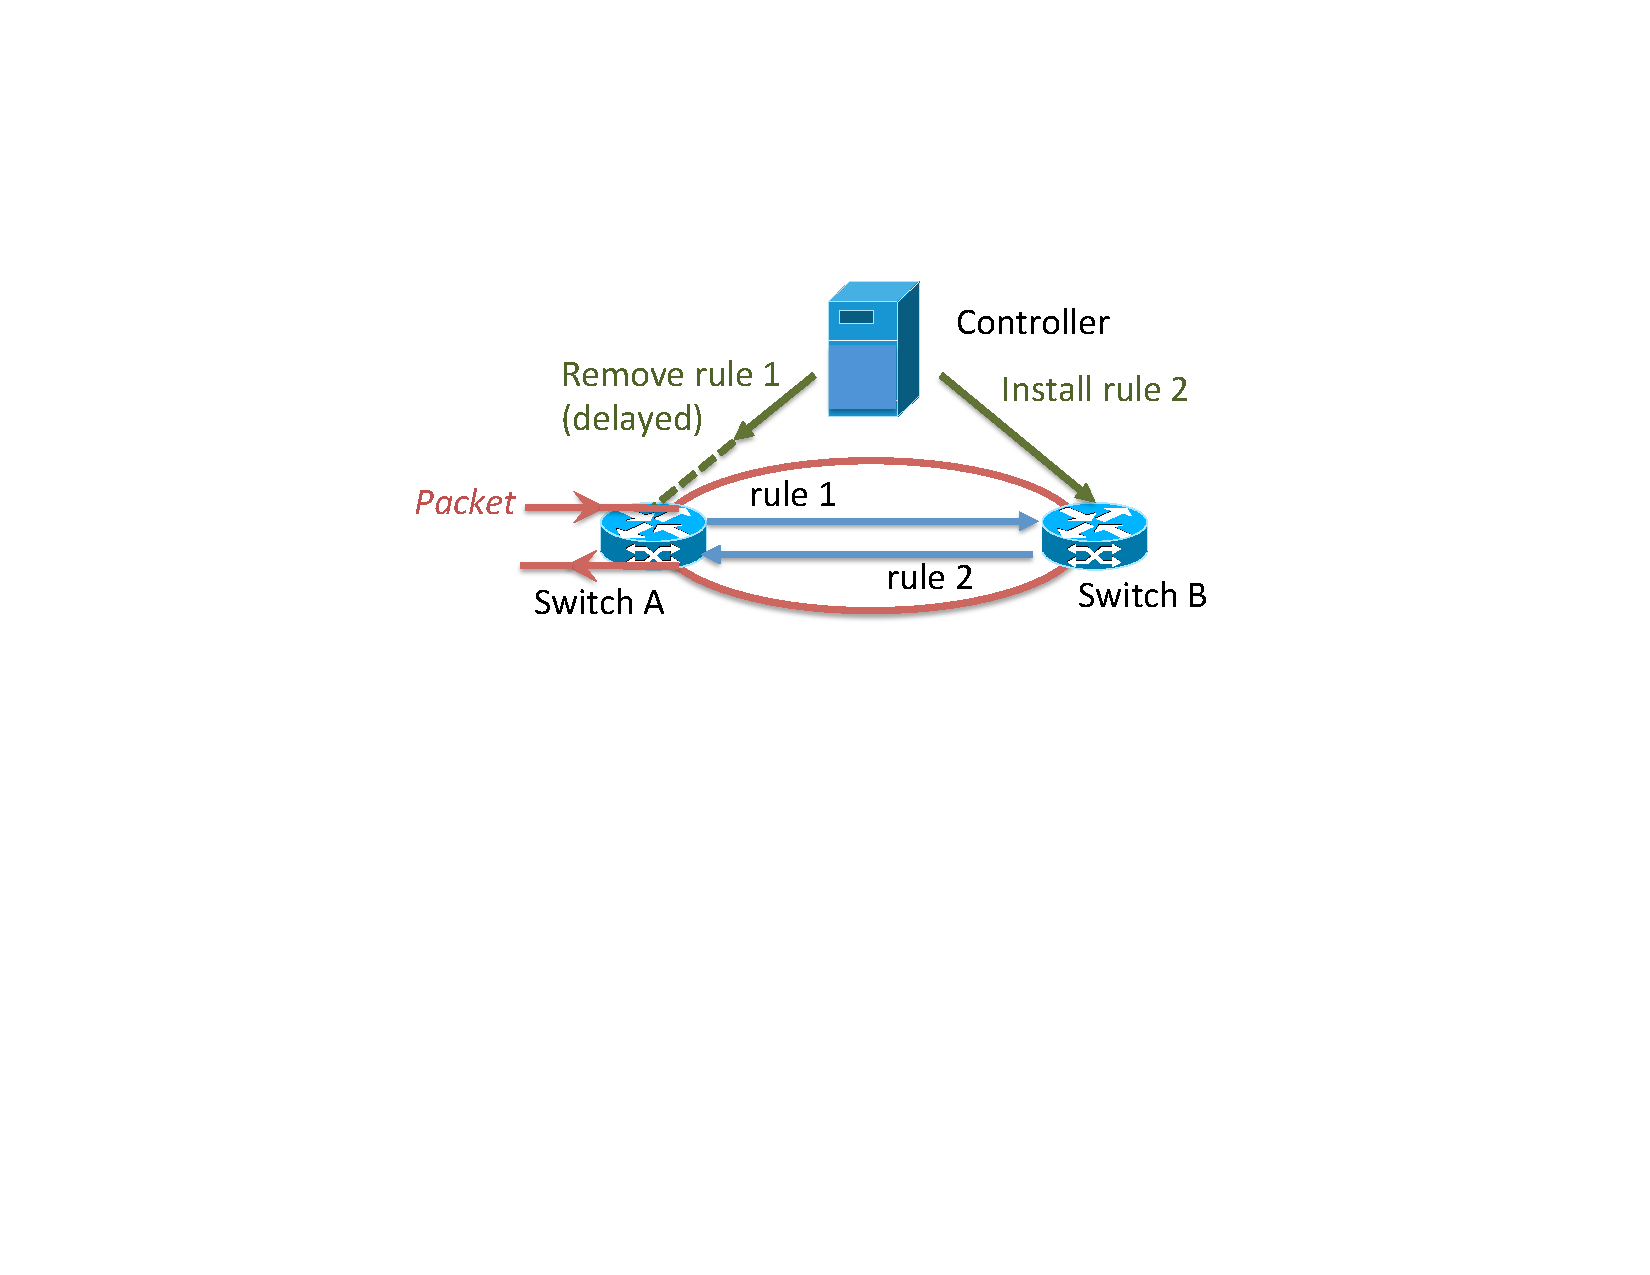
\includegraphics[width=0.7\columnwidth]{figs/example}
  \vspace{-0.1in}
  \caption{\em \small Example: challenge of modeling networks in the presence of uncertainty.}
  \vspace{-0.2in}
  \label{fig:mt_example}
\end{figure}

\if 0
Such errors may have serious consequences.  One may think such uncertainty
related errors are all transient just like the example above.  First of all,
even transient errors can be quite serious.  Take the previous example again.
a packet may enter switch $A$ while the forwarding loop exists. Note that in a
realistic deployment, switches refuse to forward packets back through
their ingress port, but drop them. So the packet will encounter a black hole $B$. 
A recent study~\cite{Flach2013} shows that TCP
transfers with loss may take five times longer to complete compared with
connections with no loss. That is, such bug may cause significant performance
drop. 
%\mattc{I feel like you should move this text up to be at the end of the "First, the bugs caused by uncertainty" paragraph -- that is where you need ot justify this.}
Regarding security issues, for instance, even temporary access control
violations can result in malicious or untrustworthy packets entering a secure
zone~\cite{Reitblatt2012}. 
%Another example is stateful firewall....
%\mattc{I do'nt get the connection bt this sentence and the previous one. Perhaps you are missing a sentence here? Are you giving an example of a temporary access contorl violation? if so why are you talking about performance?}
%\cite{OFCPP}
%\mattc{what is "the early reversing link example"? You mean the example you just gave above? If so just say "example above"}, 
%and thus, ignoring them does not matter much\mattc{don't say that! even transient bugs are very serious! a few milliseconds outage on a terabit link can affect 1000s of connections to majorly back off, harm audio, etc. this sentence weakens your case for no reason -- delete the first part and change the wording to "Even worse,.."}. 
\fi

Such errors may have serious consequences.
\wxznew{In the previous example, the resulting packet losses 
%a packet may enter switch $A$ while the forwarding loop exists,
%and thus gettting dropped there. 
%As switches typically drop packets instead of forwarding them 
%back through their ingress ports, the packet will encounter a black hole at $B$.
%Such errors could cause significant performance drop, e.g., 
could cause a significant performance drop. A recent study~\cite{Flach2013} shows TCP
transfers with loss may take five times longer to complete. 
Other transient errors could violate security policy, e.g., malicious packets could enter a secure zone because of a temporary access control violation~\cite{Reitblatt2012}.}

To make matters worse, errors caused by unawareness of network temporal uncertainty can be permanent. 
For instance, a control program initially instructs a switch to install one rule, and later removes that rule.
The two instructions can be reordered at the switch~\cite{verified-pldi13}, %so that the switch first removes a non-existing rule, 
\kevin{which ultimately causes the switch to install a rule that ought to be removed.} %resulting a state against the control program's intention. 
%Without querying the flow table at the switch, 
The view of the controller and the network state will remain inconsistent until the rule expires.
One may argue that inserting a barrier message in between the two instructions would solve the problem. 
%However, realistic cases are much more complex than this simple demonstrative example. 
%While in this case, serializing the rule installation would help eliminate the bug at the cost of performance, \mattc{don't imply things indirectly like this, it's confusing. say explicitly "
%However, serializing rules with barrier messages 
However, this may harm performance \kevin{because of increasing control traffic \wxznew{and switch operations}.} %increasing delays and control traffic. 
There are also scenarios in which carefully crafting an ordering does not help~\cite{Reitblatt2012}. In addition, %there is another question of %who should be responsible to discover this problem and to insert the barrier message.\mattc{I don't udnerstand this sentence -- isn't the controller the only option here? Maybe you mean , there's a question of 
%how the controller is able to figure out when to insert the messsages. 
\kevin{it is difficult for a controller to figure out when to insert the barrier messages.}
\name addresses that by \wxznew{serializing only updates that have potential to cause 
race conditions that violate an invariant} (\S\ref{sec:impl}).
%\mattc{btw does your algorithm help with this? If so, mention that as a possible nice use of your alg}
%\kevin{ repeated sentence: As for commonly used control programs, things are the same. 
%Three out of eleven bugs found by NICE~\cite{Nice2012}, (BUG-V, BUG-IX, and BUG-XI) are caused by the control programs' lack of knowledge of the network sate. } 

%Moreover, even if the errors disappear after a while, they could have negative impact on networks in terms of both security and performance. 
%Moreover, even transient errors can be quite serious.
%performance
%security
%An example of security issues includes 
%
%To illustrate how many potential bugs are missed when network uncertainty is neglected\mattc{This is really indirect. How about something like "
%\cut{
%Unfortunately, many SDN applications do not explicitly take into account this uncertainty. For example, network verification tools such as Veriflow assume a zero propagation delay between the controller and the network, which can lead to incorrect results. To evaluate this, we conduct measurement study, and results are shown in \S\ref{sec:bug-coverage}.
%}
%to illustrate how many potential bugs are missed if network uncertainty is neglected
%can cause performance drop. 
%in \S\ref{sec:bug-coverage}. 

\subsection{Uncertainty Model}
\label{sec:model}


%matt's comment{VF doesn’t deal with time. take into account delay, reordering.
%Control asymmetry, symbolically. Time dependent...}

%Although VeriFlow incrementally verifies the network when there are changes, and does so in real-time,



%First, using the new rule and any overlapping existing rules, we slice the network into a set of equivalence classes (ECs) of packets.

%As discussed previously, existing network verification tools do not take into account of the controller's uncertainty of the network state. But the fact is, 

%\mattc{This section starts too abruptly. when I get to this poitn I have no idea what this section is about or what you're goign ot show. Add a 1-2 sentence description of what this sec is about. Also you just jump into describing what the model is without talking about why you need a model (eg "
%To address the problem, we construct a model that accurately represents the controller's uncertainty about the network state.
%\cut{, along with a checking process to allow the controller to make decisions on when and how to send updates by checking that model. %We start by presenting the modeling technique.
%}

%For every update, assuming the controller is able to figure out whether the update is applied in the network after issuing it, there is a period of time during which the controller is uncertain about the state of the network. 

We first briefly introduce our prior work VeriFlow, a real-time network-wide \pbg{data plane} verifier.
VeriFlow intercepts every update issued by the controller before it hits the network and 
verifies its effect in real time.
VeriFlow first
slices \pbg{the set of possible packets into} Equivalence Classes (ECs) of packets
using all existing forwarding rules and the new update.
Each EC is a set of packets that experiences the same forwarding actions throughout the network.
%Because each update typically affects a very small number of ECs, 
%to limit searching space,
%VeriFlow only focuses on ECs that might be influenced by the new update. 
Next, VeriFlow builds a \emph{forwarding graph} for each EC \pbg{affected by the update,}
by collecting forwarding rules influencing the EC. 
%representing forwarding behaviors of packets belonging to those ECes.
Lastly, VeriFlow traverses each of these \pbg{graphs}
to verify network-wide invariants.

Naively, to model network uncertainty, for every update, we need two graphs to symbolically represent the network behavior with and without the effect of the update for each influenced EC, until the controller is certain about the status of the update.
%With that approach, 
If $n$ updates are concurrently ``in flight" from the controller to the network, we would need $2^n$ graphs to represent all possible sequences of update arrivals.
%Then, \kevin{\wxznew{when} \cut{for} $n$ updates concurrently ``in flight'' from the controller to the network, \wxznew{to represent} all possible sequences of update arrivals requires \cut{us to maintain} $2^n$ graphs. 
Such a state-space explosion will result in a huge memory requirement and excessive processing time to determine consistent update orderings.
%In addition, we would like to use this model to derive an algorithm to determine consistent update orderings -- executing query algorithms atop such a large amount of state would be excessive.
%, and the query time also grows proportionally. 
%Moreover, it will be really hard for operators to query possible errors in the network at any time instant with the naive approach.\wxzc{repeated errors, hard to interpret} \mattc{I don't understand the last sentence -- what do you mean by repeated errors? Why would multiple graphs be hard to interpret -- seems easier to understand than the symbolic thing you end up with in this section}

%to figure out what might go wrong.
%Therefore, we need a more efficient way to represent all possible forwarding behaviors under uncertainty. 
To address that, we efficiently model the network forwarding behavior %of each EC 
as a \emph{uncertain forwarding graph}, \pbg{whose} links can be marked as {\em certain} or {\em uncertain}.
%\mattc{shouldn't "rules" not "links" be uncertain? In fact, shouldn't uncertainty be a property for both?}
%\mattc{You never said explicitly what uncertain links are, let me add it:}
A forwarding link is {\em uncertain} if the controller does not yet have information on whether 
that corresponding update has been applied to the network.
%\cut{state yet or not}.
%\mattc{There are a lot of things here you're leaving implicit -- need to make sure reader has a complete understanding of your system, let me add:}
The graph is maintained by the controller over time. 
When an update is sent, its effect is applied to the graph and marked as uncertain.
After receipt of an acknowledgment from the network that an update has been applied
% \cut{processed by the switch} 
(or after a suitable timeout%\cut{if the SDN does not support ack'd updates}
), the state of the related forwarding link is changed to {\em certain}.
Such a forwarding graph represents all possible combinations
of forwarding decisions at all the devices.
%By inspecting the graph, the controller becomes aware of which states 
%in the network are reliably known, whether a newly arrived update from an application could result in an inconsistency with in-flight updates, and so on.

\if 0
One complication is that routers maintain multiple forwarding rules, each of which can affect
different subsets of packets. Hence, representing uncertainty on the granularity of
 physical links is not sufficient; an update may affect only one subset of packets traversing a link. Therefore, \name maintains a {\em set} of uncertainty graphs. To minimize the number of graphs we need to store,
we maintain only one graph per {\em equivalence class}, i.e., per each set of packets that undergo the same forwarding behavior 
throughout the network. Our notion of equivalence classes is similar in spirit to those used by HSA and VeriFlow, but applied to our uncertainty graph.
%\mattc{did I get this right? or do you just maintain one graph and have links for each EC?}

%We assume that there exists some mechanisms to get feedbacks from the network to confirm each controller-issued update, and the details will be discussed in \S~\ref{sec:impl}. \name stores all the possible forwarding rules in the data plane, 
%including rules that are supposed to be deleted or replaced by previously issued control messages, 
%but the deletion or replacement has not yet been confirmed, and the corresponding forwarding rules are stored as \emph{uncertain} rules. 

%When rules are collected from each device to construct a forwarding graph, 
%\name usually gets more rules compared with models that do not consider uncertainty
%\mattc{I think you should say "
%\cut{It is important to }Note that although the size of the uncertain graph could still 
%be larger than approaches that simply store a snapshot of the network,
%" -- then say why like you do below. Then at the end, poitn out "
%\cut{However, in practice, the size of this graph} 
%it is far less than storing all possible network states explicitly.
Note that it takes much less space to store the uncertainty graph than to store 
all possible network states explicitly, although it still takes more space than 
would be needed simply to store a static snapshot of the network.
%\kevin{Note that the size of the uncertain graph is far less than storing all possible network states explicitly,
%\wxznew{although it is still larger than simply storing a static snapshot of the network. }
%For example, in the OpenFlow protocol, each rule is associated with a pattern of packet header, actions to handle packets that match the pattern, and a priority to disambiguate between overlapping patterns. 
For example, an OpenFlow device typically handles an incoming packet with the highest-priority rule that the packet header matches.
%Accordingly, without considering uncertainty, %for packets of a particular pattern, the forwarding graph only takes the highest priority rule that matches that pattern at each node.
%\cut{Therefore in the graph, each node has no more than one outgoing link.}
\name collects not only the rule with the highest priority, but also the rules from the highest priority to lower priorities until a \emph{certain} rule (included) is found. This is because any rule in this collection may be used to forward packets at the moment.
%In other words, because of uncertainty, some nodes have more than one outgoing links, among which up to one is certain.
\fi

In this way, the extra storage required for uncertainty modeling is linearly bounded by the number of uncertain rules.
%, and so is the query time (\S\ref{sec:verify}). The reason is that in the worst case, there are $n$ parallel paths that need to be traversed, %instead of one without considering uncertainty, 
%where $n$ is the number of concurrent uncertain rules.
\pbg{We next examine when we can resolve uncertainty, either confirming
a link as certain or removing it.}

%``garbage collecting'' states from the graph, i.e., when one can confirm links as certain.
%That leads to the question of when it is possible to ``garbage collect'' state from the graph, i.e., when one can ``confirm'' links as being certain (\S\ref{sec:confirm}). \cut{We describe this issue in the next subsection.}

\begin{figure}[!ht]
  \centering
  \vspace{-0.1in}
  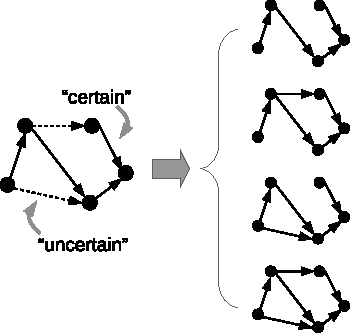
\includegraphics[width=0.6\columnwidth]{figs/model2}
  %\vspace{-0.2in}
  \vspace{-0.15in}
  \caption{\em \small \name's uncertain forwarding graph. 
%symbolic network representation provides a compact way to represent the uncertainty in a monitored network state.
  %\mattc{make this figure smaller. I feel like the size highlights it too much, it's enormous}
  }
  \vspace{-0.2in}
  \label{fig:model}
\end{figure}

\subsection{Dynamical Updating of the Model}
\label{sec:confirm}

\matt{
In order to model the most up-to-date network state, we need to update the model as changes happen in the network.
At first glance, one might think that could be done simply by marking forwarding links as uncertain when new updates are sent, and then, when an ack is received from the network, marking them as certain.
%However, \cut{there is a tricky case we need to take into account.}
%the challenge is we also need to model data packets in the network:
%\cut{In particular, the problem is that}
The problem with that approach is that it may result in inconsistencies from the data packets' perspective.}
%, e.g., even after a switch removes a rule, packets that had been processed by that rule might remain in flight.}
Consider a network consisting of four switches, as in Figure~\ref{fig:filtermoving}. %consisting of four switches operated by an SDN controller, $s_1-s_4$ (Figure~\ref{fig:filtermoving}).
%\cut{It is important to take into account these packets as well, as not doing so could introduce inconsistency issues.} \cut{-- for example, a new update installed with the assumption that all data in flight in the network is processed with existing rules could misroute or drop these existing packets, as it would not expect them to be in flight.}


%Besides modeling uncertainty with limited space, choosing a proper timing\mattc{I thought you don't use timign -- I thought you used explicit ack'ing? Maybe just say "space, determining when to confirm uncertain..."} to confirm uncertain updates is challenging too. 

%Intuitively, one may think that it is safe to change the tag of a stored rule from uncertain to certain when the feedback from the network is received at the controller. We first illustrate why that intuition is incorrect with the following example. 

\begin{figure}[!ht]
  \centering
  \vspace{-0.15in}
  %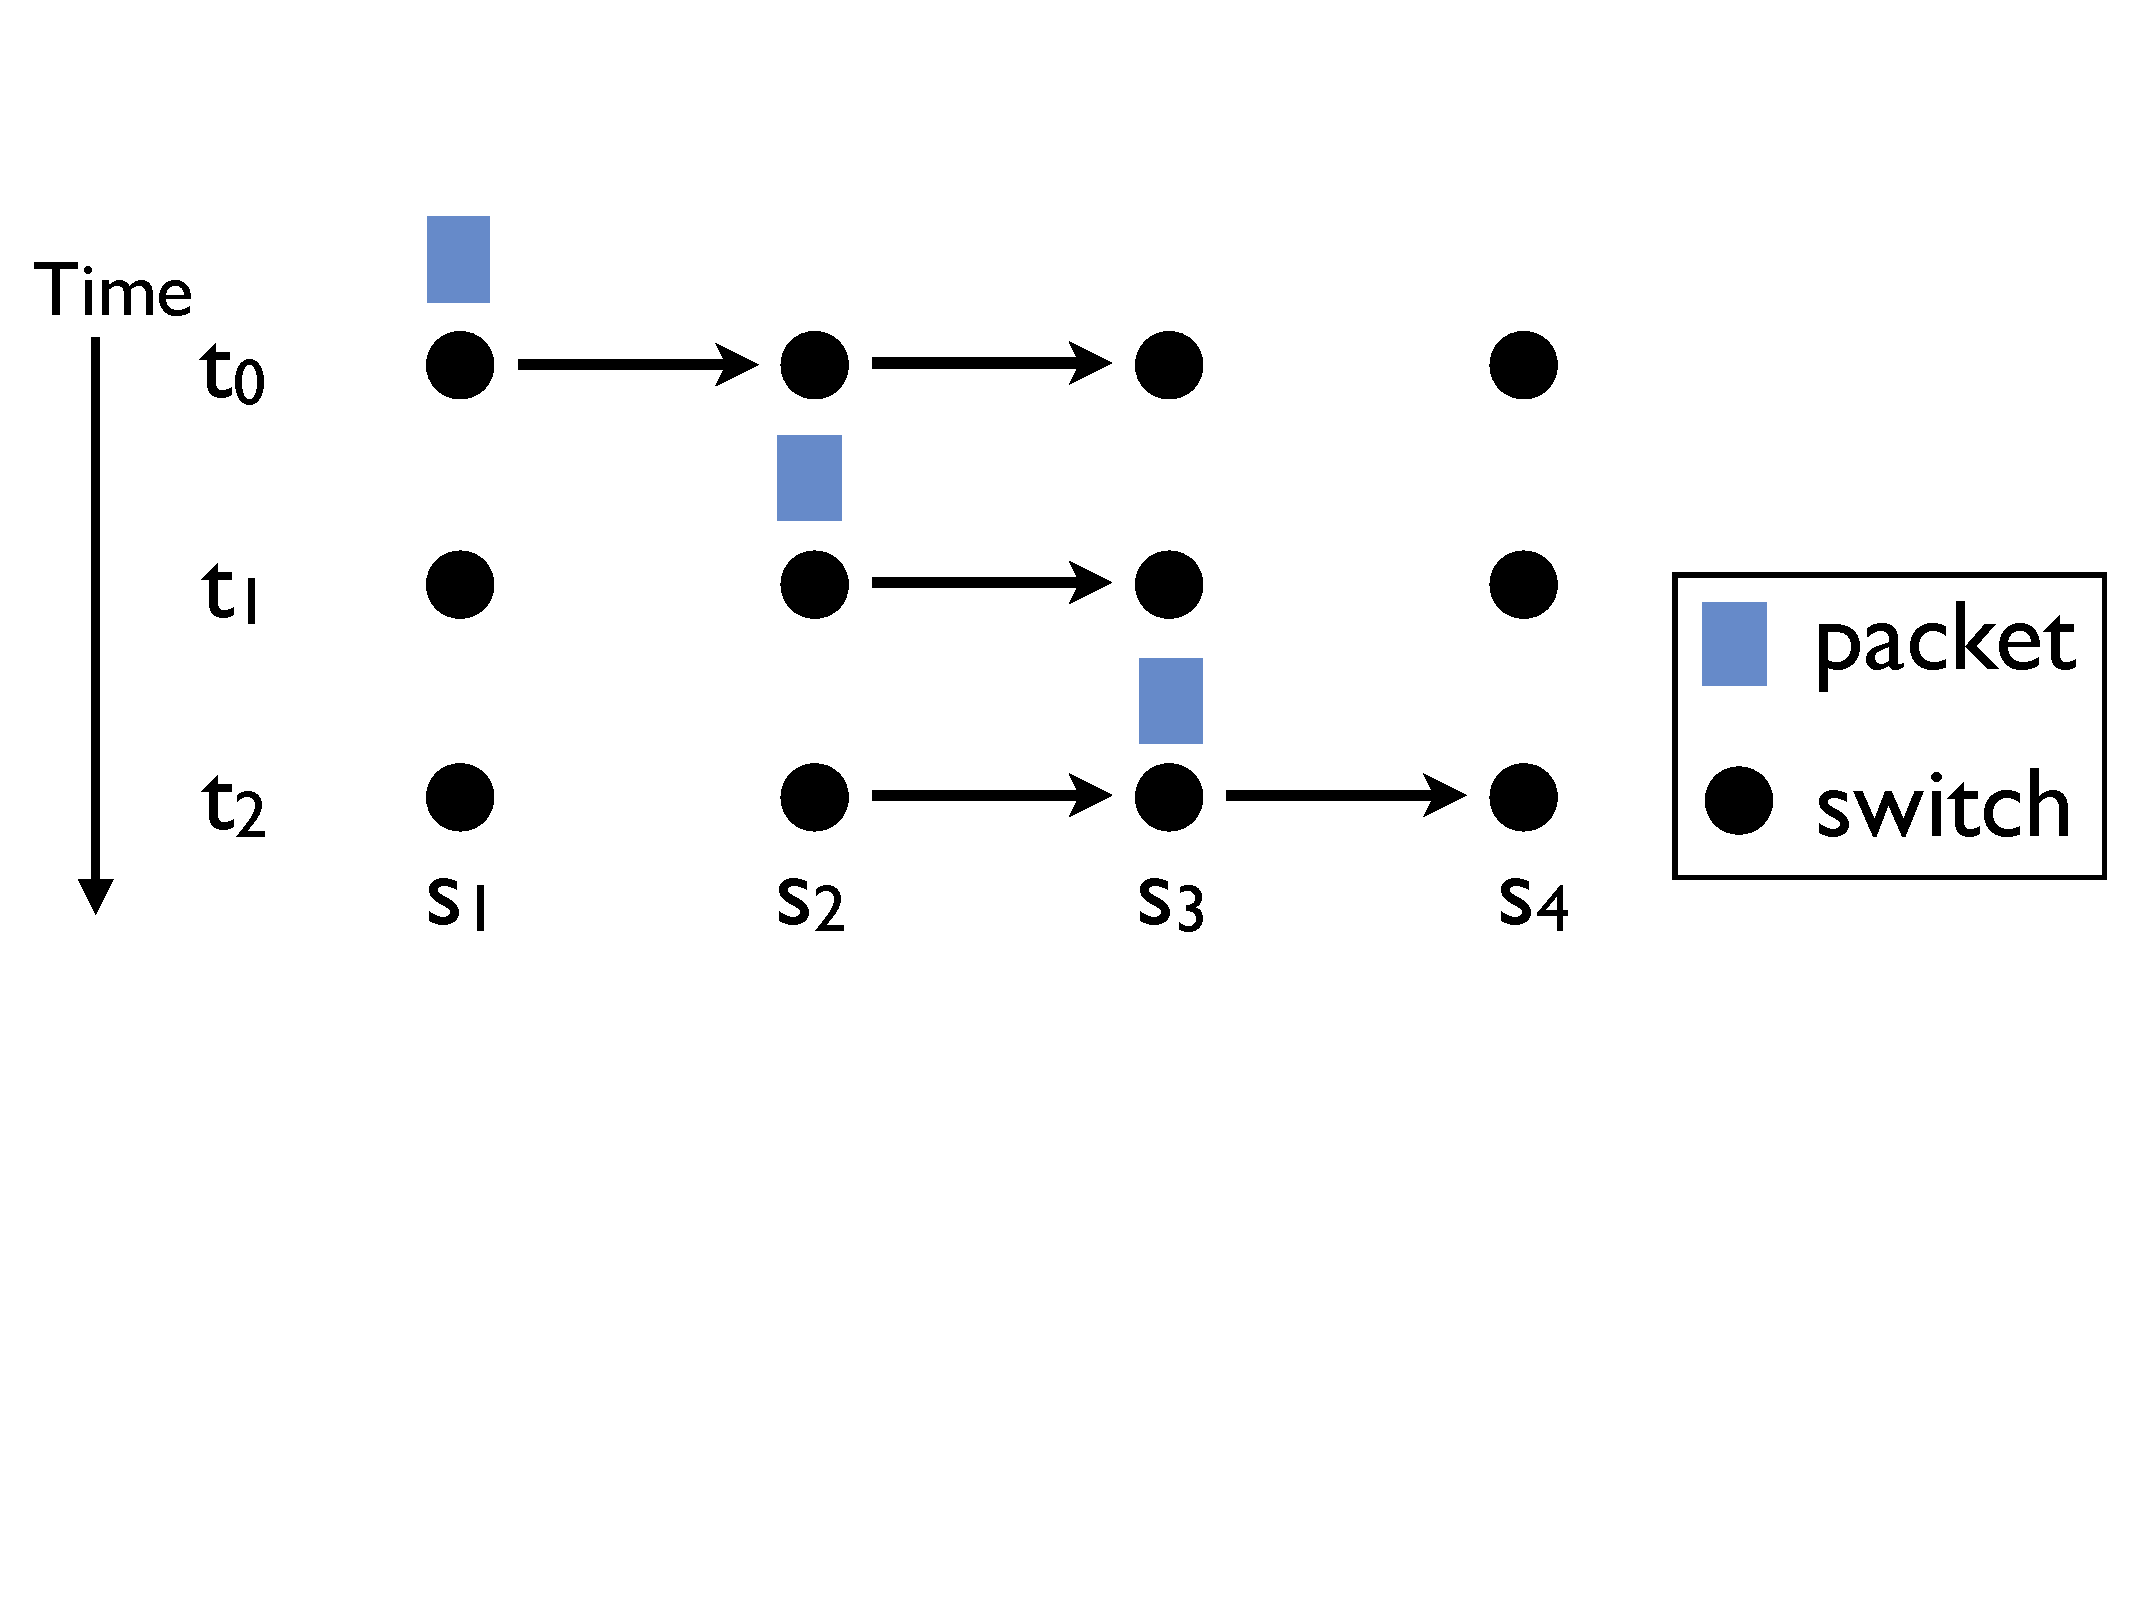
\includegraphics[width=2in]{figs/filtermoving}
  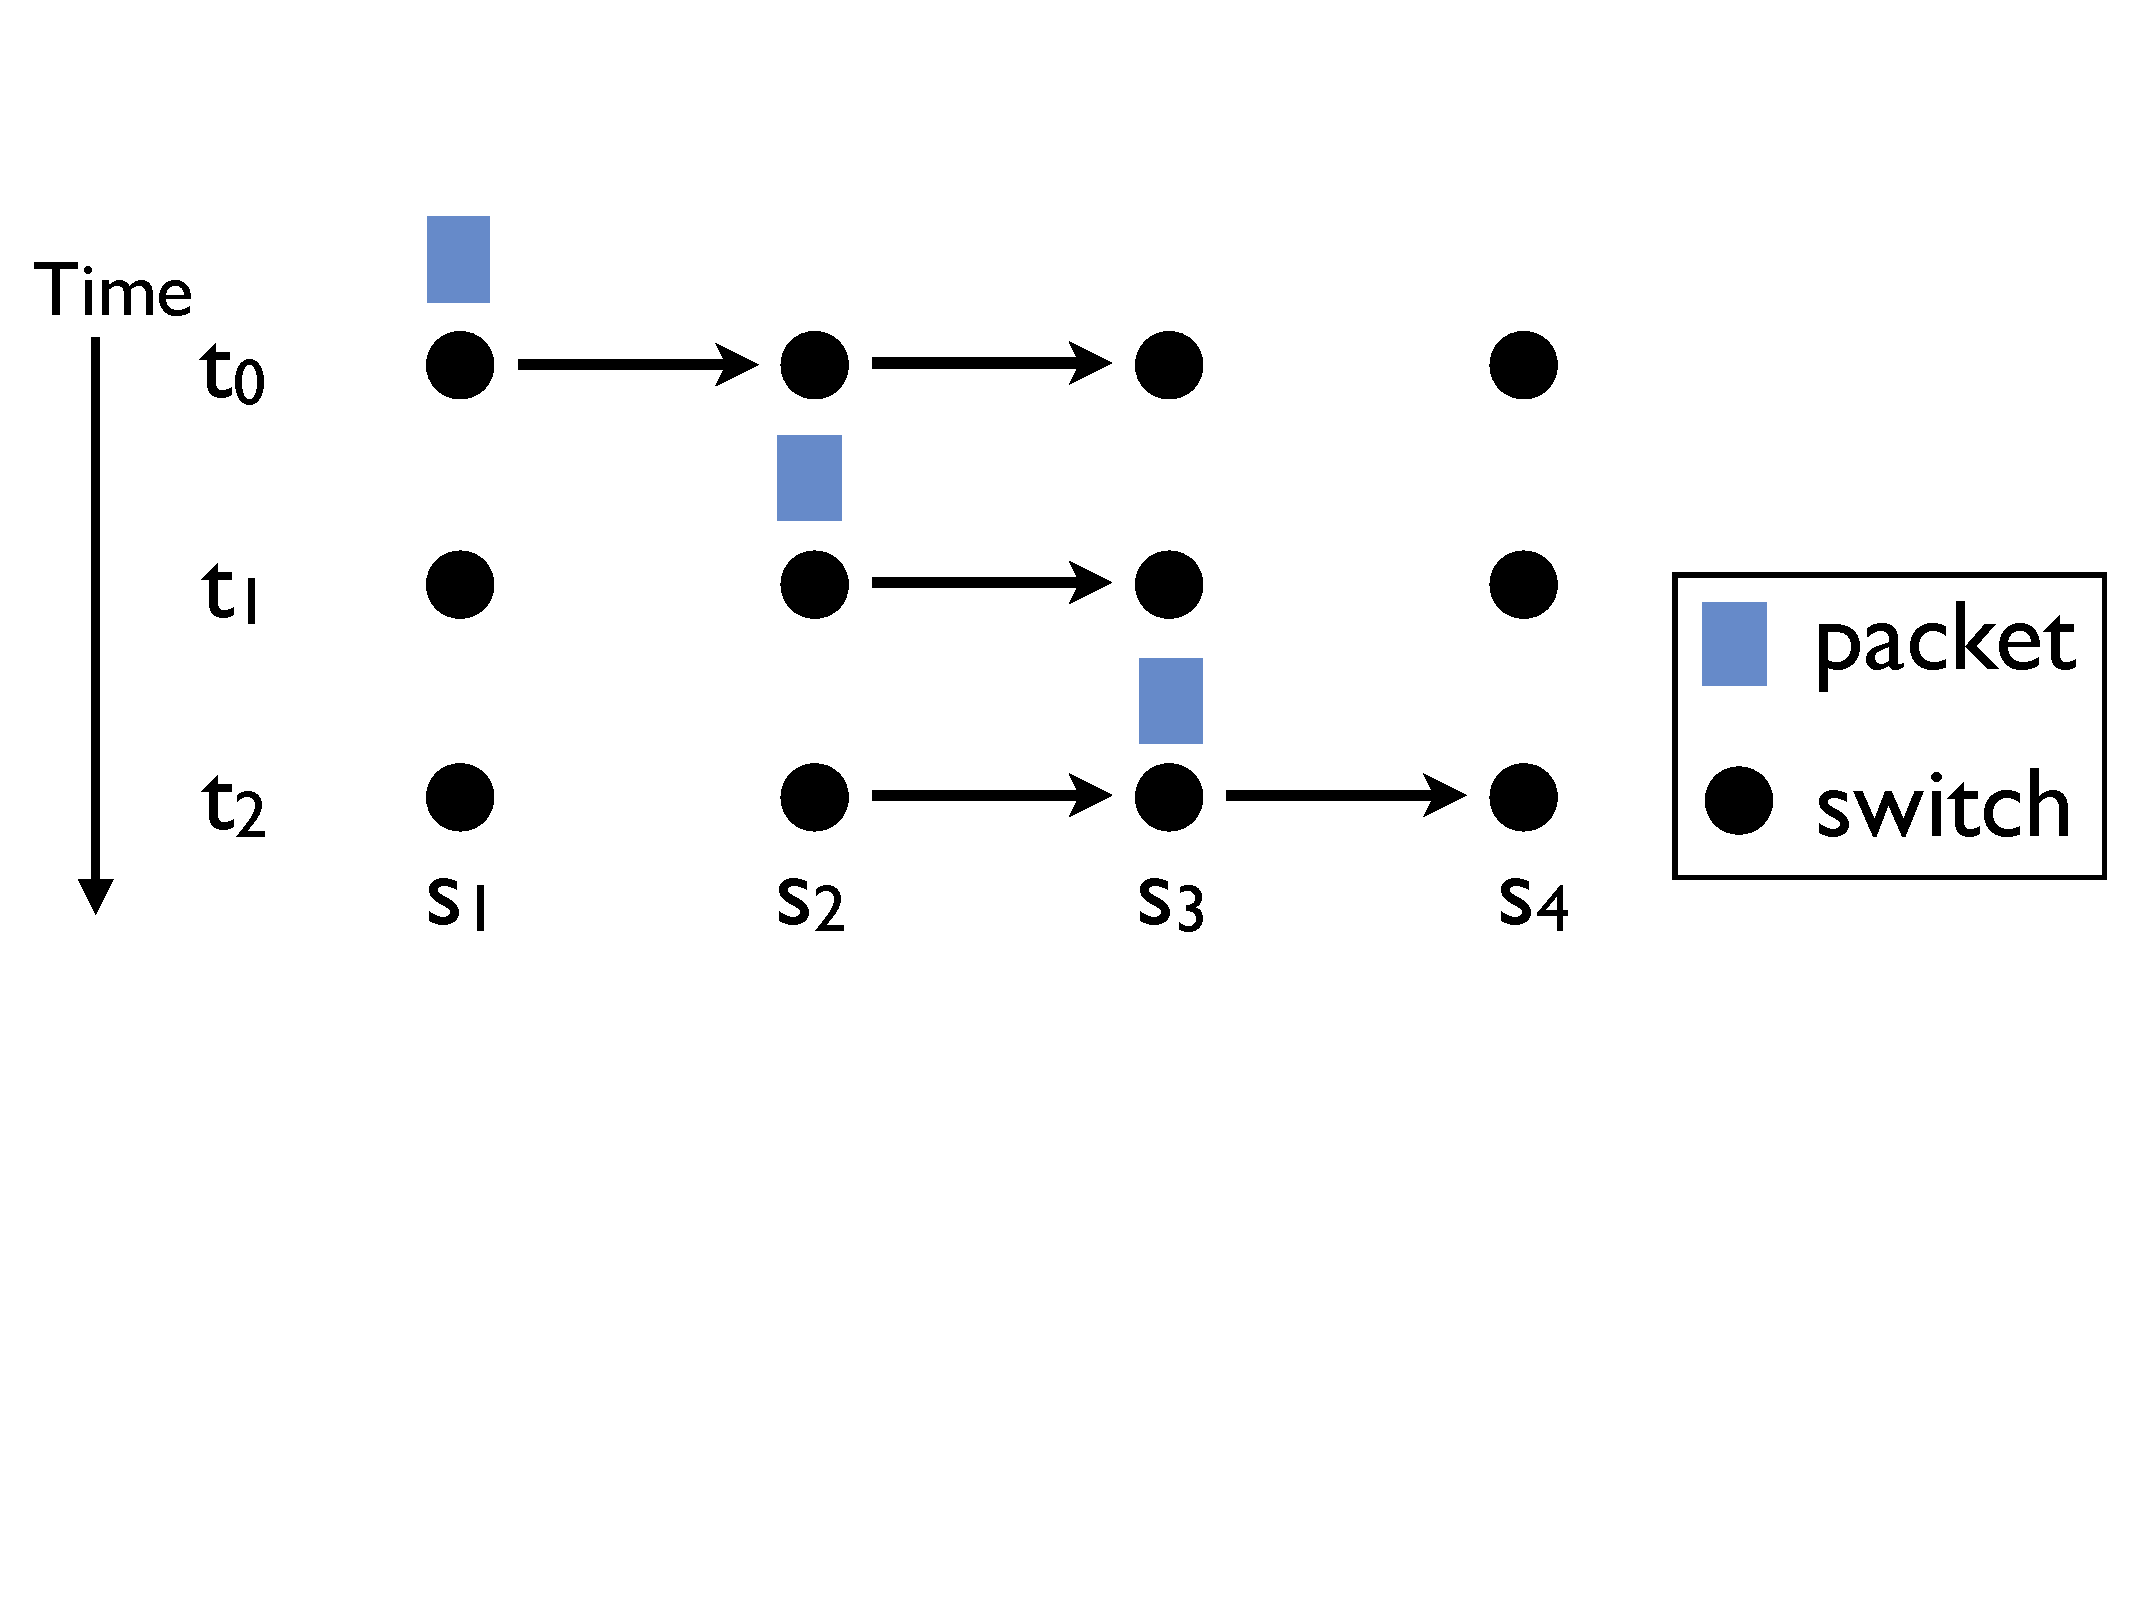
\includegraphics[width=0.8\columnwidth, trim=0mm 0mm 0mm -2mm]{figs/filtermoving}
  \vspace{-0.1in}
  \caption{\em \small Example: challenge of dealing with non-atomicity of packet traversal.}
  \vspace{-0.2in}
  \label{fig:filtermoving}
\end{figure}

%- when an ack comes back I don't process it yet - bc there's packets in flight

%\cut{To illustrate this in more detail,} 
%Let us 
The policy to enforce is that packets from a particular source entering Switch $s_1$ should not reach Switch $s_4$.
Initially, at time $t_0$, Switch $s_3$ has a filtering rule to drop packets from that source, 
whereas all the other switches simply pass packets through.
The operator later wants
%\cut{to change the configuration} 
to drop packets on $s_1$ instead of $s_3$.
%\cut{ at time $t_2$.} 
%Apparently, both the initial and final states preserve the policy.
To perform the transition in a conservative way, the controller first adds a filtering rule on $s_1$ at $t_1$, then removes the filtering rule on $s_3$ at $t_2$, after the first rule addition has been confirmed.

\kevin{The forwarding graphs at all steps seem correct.}
However, if a packet enters $s_1$ before $t_1$ and reaches $s_3$ after $t_2$, 
it will reach $s_4$, which violates the policy.
%\mattc{delete the exclamation point, and add text here saying explicitly "
\wxzcr{Traversal of a packet over the network is not atomic, 
interleaving with network updates,
as also observed in~\cite{Reitblatt2012}. 
Moreover,~\cite{bad-pkts} recently proved that there are situations where no correct update order exists.}
%Note that we are not the first to observe that problem~\cite{Reitblatt2012}.
To deal with it, upon receiving an ack from the network, \name does not immediately mark the state of the corresponding 
forwarding link as certain.
Instead, it delays application of the confirmation to its internal data structure. 
In fact, confirmations of additions of forwarding links in the graph model can be processed immediately, and only confirmations of removals of forwarding links
%\cut{in the graph model} 
need to be delayed. 
The reason is that \wxzcr{we want to ensure we represent all the possible behaviors of the network.} 
Even after a forwarding rule has been deleted, packets processed by the rule may still exist in the network, buffered in an output queue of that device, in flight, or on other devices. %That is, there are packets have this rule's footprint in their history, and for these packets, their view of the network state contains this rule throughout their lifetime in the network.
%Such confirmations include acknowledgments of deletion, expiration, or replacement by a higher-priority rule on the same device.
%\cut{
%Note that some in-flight packets handled by those forwarding links may still exist in the network. For those packets, their views of the network contain a subset of those non-existing links. }

%\cut{To decide that}
%As for how long confirmations should be delayed, 
%\wxzcr{as in past work~\cite{Reitblatt2012, incremental-cu}},
%one way is to use a fixed timeout, assuming we have an estimation of 
%the upper bound of packet- or flow-level traversal latency.
%After such a delay, all packets that may be handled using the old state are drained off the network. 
%Another possible way is to actively query the network to see if the packet or flow leaves the network.
%asking network devices to include queue length 
%related to the new update in the feedback messages.
%Based on the queue length, we can calculate the maximum delay for 
%packets using the previous configuration to leave the network.
%More details of how the state of a rule can be changed in our model are presented in \S\ref{sec:statemachine}.
We have proved that our uncertainty-aware model is able to accurately 
capture the view of the network from the packets' perspective~\cite{gcc_tr},
\wxzcr{even for in-flight packets that have been affected by rules not currently present}.
  \vspace{-0.1in}
\begin{definition} A packet $P$'s view of the network \pbg{{\bf agrees}} with
the uncertainty-aware model, if at any time point during its traversal of the
network, the data plane state that the packet encounters is in the model at
that time point. More specifically, at time $t$, to $P$ if a link $l$
\begin{itemize}[noitemsep,topsep=0pt,leftmargin=*] 
\item is reachable, $l$ is in the graph model for $P$ at $t$;
\item otherwise, $l$ is definitely not certain in the graph at $t$.
\end{itemize} \end{definition}
  \vspace{-0.1in}

  \vspace{-0.1in}
\begin{theorem} Assuming that all data plane changes are initiated by the controller,
any packet's view of the network \pbg{agrees} with the uncertainty-aware model.
\end{theorem}
  \vspace{-0.1in}
\if 0
  \vspace{-0.1in}
\begin{proof} Without loss of generality, assume that the maximum duration of a
packet in the network is $\delta$, which is set as the amount of delay added to
confirmations.  Consider a packet $P$ that enters the network at time $t_1$ and
leaves at $t_2$ ($t_2-t_1 \le \delta$).  Assume that $P$ traverses the network in
$n$ hops, and when $n=0$, $P$ enters the network.  Clearly the theorem holds for
$n=0$.  Consider hop $k, (k \ge 0\mbox{ and } k \le n)$.  By induction, at
hop $(k-1)$, assume that $P$'s view is consistent with the model.

If $P$ encounters a forwarding link at hop $k$, then there exist two cases.
In case 1, the corresponding forwarding rule is intentionally inserted by the
controller, and by the time $P$ reaches hop $k$, the rule is installed.  In case
2, the rule is about to be removed, but the action is not done until $P$ has been
handled by the rule.  Let $t_i$ denote the time of issuing the related command (to add or
remove the rule), and $t_c$ the time it is confirmed at the controller as.  
In case 1, since $P$ reaches the link, $t_i < t$.  In the model, that
link is modeled as either certain ($t_c \le t$) or uncertain ($t_c > t$).  In
case 2, because the link is reachable to $P$ at $t$, in $P$'s lifetime $[t_1,
t_2]$, $P$'s view of the network state contains that link.  $t_c$ cannot be
earlier than $t$, because if it were, $P$ could not reach the link.  Because of the delayed
confirmation mechanism, if an update $u$ causes the removal of the link, the
status of the rule remains as uncertain for an extra $\delta$ time in the model
until $t_c + \delta > t_2$, which is consistent with $P$'s view.  
%(even if the
%acknowledgement of applying $u$ reaches the controller at $T_c$ before $t_2$).
In particular, if $t_i \ge t$, then the link is included as certain in the model
until the update is issued ($t_i$).

If $P$ reaches a location where no forwarding rule is available, there are also
two cases.  In case 1, some forwarding rules have been issued to handle $P$ at this
location, but they have not been applied yet. In case 2, there had been available rules, but
they were removed before $t$.  In case 1, $t_c$ is definitely later than $t$.
If it weren't, the rule would be there by $t$.  If $t_i < t$, at $t$, the forwarding rule
is only modeled as uncertain.  If $t_i \ge t$, at $t$, the model does not
contain that rule.  In case 2, the removal of the rules is issued before $t$.
In the interval $[t_i, t_c + \delta]$, any rule $R$ is modeled as uncertain,
and after the interval, $R$ is removed from the model, after $P$ leaves the
network.  Hence, the model is consistent with the view of $P$ during its
lifetime in the network.
\end{proof}
\fi
%Note that in practice, only {\em certain} and {\em uncertain} two states are not sufficient (e.g., whether to mark a link as certain can depend on subsequent updates), but we here skip the details.
%\footnote{This theorem is proved in a technical report that has been mailed to the program committee chairs.}


\subsection{Uncertainty-aware Verification}
\label{sec:verify}
\cut{
\matt{
As a demonstration of one possible use of our model, we give an application of it in developing a network verification tool.
Recently, several network verification systems for SDN have been proposed.
For example, VeriFlow~\cite{VeriFlow} constructs an efficient model of the network under consideration, and performs high-speed traversals
of the model to analyze reachability properties.
Unfortunately, VeriFlow assumes that the delay between the controller and the network is zero --- this can cause it to give incorrect results (both false positives
and false negatives). We show more detailed results and examples of these incorrect results in \S\ref{sec:bug-coverage}.
}
}
%as demonstration, we show how this helps correctly perform verification in distributed settings}
%\if 0 %matt: why was this commented out?
%After obtaining a model that captures all possible network states,
%we will then verify that model against desired properties.
%Given a desired network invariant and a (group of) update(s),
%\name traverses the uncertain forwarding graphs,% of ECs affected by the update(s),
%using directed graph algorithms, to verify against the invariant.
%Uncertain links and certain links need to be treated differently.
%For example, if the traversal reaches a node with no \emph{certain} outgoing links,
%it is possible that packets %of the corresponding EC 
%encounter a black-hole even with multiple \emph{uncertain} outgoing links available,\mattc{missing text here? needs a few more sentences of detail}.
%\fi
\kevin{Construction of a {\em correct} network verification tool is straightforward with our uncertainty-aware model.}
By traversing the uncertainty graph model using directed graph algorithms, we can 
%infer 
\wxzcr{answer queries such as whether a reachable path exists between a pair of nodes.}
That can be done in a manner similar to existing network verification tools like HSA \cite{NetPlumber2013} and VeriFlow \cite{VeriFlow}.
However, the traversal process needs to be modified to take into account uncertainty.
When traversing an uncertain link, we need to keep track of the fact that downstream inferences lack certainty.
%This is done by \mattc{add a few technical sentences here with details -- give the exact traversal algorithm in words}
% uncertain links and certain links need to be treated differently.
If we reach a node with no \emph{certain} outgoing links,
it is possible that packets will encounter a black-hole even with multiple \emph{uncertain} outgoing links available.
%Thus, we are able to answer queries by traversing the graph once. 
\wxzcr{By traversing the graph once, \name can reason about the network state correctly in the presence of uncertainty, determine if an invariant is violated, and output the set of possible conterexamples (e.g., a packet and the forwarding table entries that caused the problem).
}
%\matt{
%Like Veriflow, \name can determine whether a supplied invariant is violated, and if so, output a counterexample (e.g., a packet and the forwarding table entries that caused the problem).
%Unlike Veriflow, \name can also reason correctly in the presence of uncertainty. 
%%If the analysis can be conducted with certainty, \name outputs the result. If it cannot (e.g., 
%If multiple possible network states exist, \name can output the set of possible different answers.
%\cut{
%Knowing if there existed a possibility an invariant was violated (regardless of whether it actually happened) is still quite useful information --- application designers
%may wish to learn about and fix such race conditions in their designs, and knowing that there is a chance a vulnerability was exploited can inform operators to conduct
%more extensive investigations.
%}
%By keeping track of which links are uncertain, we can also indicate the degree of confidence in the result -- in particular,
%if a supplied invariant is violated, our tool, like Veriflow, can output the 
%}

% \subsection{Verification}
% \label{sec:verify}
% \matt{
% As a demonstration of one possible use of our model, we give an application of it in developing a network verification tool.
% Recently, several network verification systems for SDN have been proposed.
% For example, Veriflow~\cite{VeriFlow} constructs an efficient model of the network under consideration, and performs high-speed traversals
% of the model to analyze reachability properties.
% Unfortunatley, Veriflow assumes that the delay between the controller and the network is zero --- this can cause it to give incorrect results (both false positives
% and false negatives). We show more detailed results and examples of these incorrect results in Section~\ref{sec:bug-coverage}. 
% }

% Using our model, constructing a {\em correct} network verification tool is relatively straightforward.
%as demonstration, we show how this helps correctly perform verification in distributed settings}
% \if 0
% After obtaining a model that captures all possible network states,
% we will then verify that model against desired properties.
% Given a desired network invariant and a (group of) update(s),
% \name traverses the uncertain forwarding graphs,% of ECs affected by the update(s),
% using directed graph algorithms, to verify against the invariant.
% Uncertain links and certain links need to be treated differently.
% For example, if the traversal reaches a node with no \emph{certain} outgoing links, 
% it is possible that packets %of the corresponding EC 
% encounter a black-hole even with multiple \emph{uncertain} outgoing links available,\mattc{missing text here? needs a few more sentences of detail}.
% \fi
% 
% \matt{
% By traversing the uncertainty graph model using directed graph algorithms, we can infer whether a reachable path exists between a pair of nodes.}
% Note that during traversals, 
% uncertain links and certain links need to be treated differently.
% For example, if the traversal reaches a node with no \emph{certain} outgoing links, 
% it is possible that packets %of the corresponding EC 
% encounter a black-hole even with multiple \emph{uncertain} outgoing links available.
% %,\mattc{missing text here? needs a few more sentences of detail}.
% \matt{
% Like Veriflow, our tool can determine if a supplied invariant is violated, and if so, output a counterexample (e.g., the specific set of forwarding
% table entries that cause the problem).
% Besides, our tool can also reason accurately in the presence of uncertainty -- if the analysis can be conducted accurately on the graph, our tool
% outputs the result. If it cannot (e.g., if multiple possible network states exist), our tool can output the set of possible different answers.
% Knowing if there existed a possibility an invariant was violated (regardless of whether it actually happened) is still quite useful information --- application designers
% may wish to learn about and fix such race conditions in their designs, and knowing that there is a chance a vulnerability was exploited can inform operators to conduct
% more extensive investigations.
% %By keeping track of which links are uncertain, we can also indicate the degree of confidence in the result -- in particular,
% %if a supplied invariant is violated, our tool, like Veriflow, can output the 
% % }
% In this way, we are able to model the network states accurately using a single graph,% per EC, 
% and answer queries by traversing the graph once. The extra storage \name requires due to uncertainty modelling is linearly bounded by the number of uncertain rules, and so is the query time. It is because that in the worst case, there are $n$ parallel paths that need to traverse instead of one without considering uncertainty, where $n$ is the concurrent uncertain rules.
% 

\if 0
\subsection{Proof of Correctness}
\label{sec:proof}

Let us illustrate that the uncertainty-aware model can accurately capture the view of the network from packets' perspective. First, we define the situation when the view of a packet is consistent with the uncertainty network model. 

\begin{definition}
A packet $P$'s view of the network is {\bf consistent} with the uncertainty-aware model, if at any time point during its traversal of the network, the data plane state that the packet encounters is in the model at that time point. More specifically, if a link is reachable for $P$ at time $t$, then that link is included in the model at $t$.
Whereas if a link is unreachable for $P$ at $t$, then that link is definitely not certain in the model at $t$.
\end{definition}

\begin{theorem}
Assume no physical failures change the data plane, for any packet, its view of the network is consistent with the uncertainty-aware model. 
\end{theorem}

\begin{proof}
Without loss of generality, assume the maximum duration of a packet in the network is $\delta$, which is set as the amount of delay added to confirmations.
Suppose that packet $P$ enters the network at time $t_1$ and leaves at time $t_2$, so $t_2-t_1 \le \delta$.
Also assume $P$ traverses the network in $n$ hops, while when $n=0$, $P$ enters the network.
Clearly it holds for $n=0$. 
Consider hop $k, (k \ge 0\mbox{ and } k \le n)$.
By induction, at previous hop $(k-1)$, $P$'s view is consistent with the model.

If $P$ encounters a forwarding link at hop $k$, then there exist two cases.
In case 1, the corresponding forwarding rule is intentionally inserted by the controller, 
and by the time $P$ reaches hop $k$, the rule is installed.
Case 2, the rule is about to be removed, but the action is not done until $P$ is handled by the rule.
Let us denote the time of issuing the related command (to add or remove the rule) as $T_i$
, and the time that the confirmation arrives at the controller as $T_c$.
In case 1, since $P$ reaches the link, $T_i < t$.
In the model, that link is modeled either as certain ($T_c \le t$) or uncertain ($T_c > t$).
In case 2, because the link is reachable to $P$ at $t$, 
in $P$'s life time $[t_1, t_2]$, its view of the network state contains that link. 
$T_c$ cannot be earlier than $t$, otherwise $P$ could not reach the link.
Due to the delayed confirmation, if an update $u$ causes the link removal, the status of the link remains as uncertain for extra $\delta$ time in the model, which is consistent with $P$'s view (even if the acknowledgment of applying $u$ reaches the controller at $T_c$ before $t_2$). Specially, if $T_i \ge t$, then the link is included as certain in the model until the update is issued ($T_i$).

If $P$ reaches a location where no forwarding rule is available, there are also two cases. 
In case 1, some forwarding rules are issued to handle $P$ at this location, but not applied yet.
In case 2, there were available rules, but the rules were removed before $t$.
In case 1, $T_c$ is definitely later than $t$, otherwise the rule is in the data plane by $t$. 
If $T_i < t$, at $t$, the forwarding rule is only modeled as uncertain.
If $T_i \ge t$, at $t$, the model does not contain that rule.
In case 2, the removal of any rules is issued before $t$.
In the interval $[T_i, T_c + \delta]$, any rule $R$ is modeled as uncertain, 
and after the interval, $R$ is removed from the model, which makes the model consistent with the view of $P$ during its life time in the network.
\end{proof}
\fi

%Clearly it holds for time earlier than $t_1$ or later than $t_2$.
%For the sake of simplicity, we confine our discussion here within updates overlapping with %the EC that 
%packet header space of $f$.% belongs to.
%Updates confirmed earlier than $t_1$ or issued later than $t_2$ are certainly applied or not applied, 
%and thus they don't alter during the presence of $f$.
%While updates issued or confirmed between $t_1$ and $t_2$, named as set $U$, have the potential to change the state $f$ encounters.
%For any update $u$ in $U$, before its issuing time, it is neither in the data plane or able to touch any packet of $f$.
%After $u$ is issued, it's possible that $u$ handles some packets from $f$ until $f$ completely leaves the network, at $t_2$.
%Due to delay of confirmation, if $u$ causes removal of a link in the uncertainty model, 
%even if the acknowledgment of applying $u$ reaches the controller at $t_c$ before $t_2$, 
%the status of $u$ remains as uncertain for $\delta$. 
%Because $ t_c + \delta \ge t_2 $, until $f$ is gone, any possible situation that $f$ may met is modeled in the uncertainty graph.

%Model: Channels + processors   

%Define \emph{Certain Path}: a path consists of only certain links.
%
%%1. Given a EC, 
%1. If a path is traversable in the data plane, there must exist the same path in the graph model.% of that EC.
%
%Proof. any forwarding rule that is possibly in the data plane is stored in the model as certain or uncertain. 
%For each hop of the path, the forwarding rule is modeled as a link in the graph model.
%
%2. Assuming no physical failures, %given an EC, 
%if two nodes are not connected in the data plane, 
%there is no \emph{certain path} between them in the model.
%
%Proof. By contradiction, if there is a certain path connecting the two nodes, every link in the path corresponds a forwarding rule certainly installed in the data plane. Then the two nodes are connected in the data plane.
%
%Define \emph{Uncertainty Coherence} If a forwarding state graph can be mapped as a subgraph of an uncertainty forwarding graph, and links in the uncertainty graph but not in the forwarding state are all uncertain, this forwarding state is \emph{coherent} with the uncertainty graph. 
%
%3. At any time point, the current data plane state %for any EC 
%is coherent with %this EC's 
%the uncertainty graph model.
%
%From 1 and 2.
%
%
%Without loss of generality, assume the system requires a flow level consistency, 
%and the maximum duration of a flow in the network is $\delta$, which is set as the amount of delay added to confirmations.
%
%
%4. Any flow's instantaneous view of the network is coherent with the uncertainty graph model, %of the EC to which this flow belongs, 
%although it may not conherent with the data plane state.
%
%Proof. Suppose a flow $f$ enters the network at time $t_1$ and leaves at time $t_2$, so $t_2-t_1 \le \delta$. 
%Clearly it holds for time earlier than $t_1$ or later than $t_2$.
%For the sake of simplicity, we confine our discussion here within updates overlapping with %the EC that 
%packet header space of $f$.% belongs to.
%Updates confirmed earlier than $t_1$ or issued later than $t_2$ are certainly applied or not applied, 
%and thus they don't alter during the presence of $f$.
%While updates issued or confirmed between $t_1$ and $t_2$, named as set $U$, have the potential to change the state $f$ encounters.
%For any update $u$ in $U$, before its issuing time, it is neither in the data plane or able to touch any packet of $f$.
%After $u$ is issued, it's possible that $u$ handles some packets from $f$ until $f$ completely leaves the network, at $t_2$.
%Due to delay of confirmation, if $u$ causes removal of a link in the uncertainty model, 
%even if the acknowledgment of applying $u$ reaches the controller at $t_c$ before $t_2$, 
%the status of $u$ remains as uncertain for $\delta$. 
%Because $ t_c + \delta \ge t_2 $, until $f$ is gone, any possible situation that $f$ may met is modeled in the uncertainty graph.

%Model: Channels + processors   
%	Assumption: 
%1)	infinite flow table size → no eviction due to lack of space
%we assume that flow tables on switches can be arbitrarily large. This is not the case for hardware switches, where the size of flow tables is often constrained by the amount of silicon used, and varies from switch-to-switch. It would be straightforward to modify our model to bound the size of the table on each switch. 
%2)	no failure
%3)	no congestion caused pkt drop (infinite queue length)
%
%Modeling the state space. A distributed system consists of multiple components that communicate asynchronously over message channels, i.e., first-in, first-out buffers (e.g., see Chapter 2 of [19]). Each component has a set of variables, and the component state is an assignment of values to these variables. The system state is the composition of the component states. To capture in-flight messages, the system state also includes the contents of the channels. A transition represents a change from one state to another (e.g., due to sending a message). At any given state, each component maintains a set of enabled transitions, i.e., the state’s possible transitions. For each state, the enabled system transitions are the union of enabled transitions at all components. A system execution corresponds to a sequence of these transitions, and thus pecifies a possible behavior of the system.   
%
%	For each packet that traverses the network before/after an uncertain period, models the exact behavior
%	For each packet that traverses the network within an uncertain period, models all possible behaviors
%	E.g. FIFO channel
%S, e, s, e…
%Send, receive event                                     
%any time T, any pkt p, 
%	if p is @switch S
%		if  S’s corresponding forwarding rule is certain…
%		if not, then the FG has all the uncertain choices
%	if p is in channel C (in-flight)
%		1) if S has been certain for a while, …
%		2) if S has an update lately but is certain now, p might be put in the buffer before the update is confirmed.
%3) If S uncertain
%in case 2) and 3) p encounters uncertainty at S
%by delaying confirmation in FG by the queuing delay, such uncertainty is depicted in the FG. 
%
%(As a byproduct, this can model in-network congestion events, as long as there’s no pkt drop)			
%
%For flow table/topology changes originated from the network, e.g., failure/soft timeout, we can model the historical uncertainty by looking back. Assuming a one-way delay threshold T, from t-T to t, it is uncertain.
%
%What we didn’t cover in the modeling: (events initiated from the network)
%1.	failure
%2.	congestion(?)
%3.	timeout…
%(ATPG)
%
%
%\subsection{Invariant Expression}
%\label{sec:ctl}
%configurechecker
%

%\begin{figure*}[t]
%  \centering
%  \mbox{
%    \subfigure[]{{\includegraphics[width=2.2in]{figures/planetlab-evaluation/cache/cache.pdf}}}
%    \subfigure[]{{\includegraphics[width=2.2in]{figures/planetlab-evaluation/ncache/ncache.pdf}}}
%    \subfigure[]{{\includegraphics[width=2.2in]{figures/planetlab-evaluation/random-adns/random-adns.pdf}}}
%  }
%  \vspace{-0.1in}
%  \caption{\small \em
%      Overall download time, when DNS caching is (a)~enabled, bypassing the ADNS; (b)~disabled, with the ADNS colocated with the server; and
%    (c) disabled, with the ADNS in a random location.
%    \vspace{-0.2in}
%  }
%  \label{fig:latency}
%\end{figure*}

%\begin{figure}[t]
%  \centering
%  {{\includegraphics[width=2.3in]{figures/overhead/oh_scp.pdf}}}
%  \caption{\small \em
%    Cryptographic overhead.-
%  }
%  \label{fig:comp}
%\end{figure}


%section{Maximizing Parallelism}

%\section{Verification and Consistency under Uncertainty}
\section{Consistency under Uncertainty}

%The previous sections described our modeling approach.
\if 0
In this section, we describe how to leverage our model to build useful tools.
First (\S\ref{sec:verify}), we describe how our model can be used to perform
safe, uncertainty-aware network verification.
Then (\S\ref{sec:parallelism}~\S\ref{sec:synthesis}), we describe how to 
leverage our model to efficiently synthesize update sequences
that obey a set of provided invariants.
\fi
\kevin{
Now we describe how we use our model
%to perform
%uncertainty-aware network verification (\S\ref{sec:verify}),
%then 
to efficiently synthesize update sequences that obey a set of provided invariants (\S\ref{sec:parallelism}). Next, we identify the scope of invariants that can be guaranteed with heuristically maximized updating speed (\S\ref{sec:seg-independence}), and present our technique to preserve consistency for the remaining invariants (\S\ref{sec:synthesis}).}


\subsection{Enforcing Correctness with Maximized Parallelism}
\label{sec:parallelism}

%\cut{
%The previous section described how to verify network correctness, with general invariants, using our model.
The key goal of our system is to {\em instill}
%flexible and 
user-specified notions of correctness during network transitions.
%Doing this can ensure networks {\em continuously} obey general consistency properties
%even during network changes, and 
%even while the state of the network is converging. 
%\wxzc{what does "even while the state of the network is converging" mean?}

Using our model to perform this task is also relatively straightforward.
%In particular, 
We can construct a {\em buffer} of updates received from the application,
and attempt to send them out in FIFO order. Before each update is sent, we check with the
verification engine on whether there is any possibility, given the uncertainty in network state, sending it could result in an invariant violation. If so, the update remains buffered until it is safe to be sent.

There are two key problems with this approach.
The first is head-of-line blocking: it may be safe to send an update, but one before it in the queue, which isn't safe, could block it. This introduces additional delays in propagating updates
to the network.
%, which slows the convergence process and reaction to events.
Second, only one update is sent at a time, which is wasteful---if groups of updates do not conflict with each other, they could be sent in parallel.

To address this,
%\cut{As the ultimate goal of our system is t}To {\em instill} flexible and user-specified notions of correctness during network transitions,
\name provides an algorithm for synthesizing update sequences to networks that greedily {\em maximizes parallelism} while
simultaneously obeying \wxznew{the supplied}\cut{flexible consistency} properties
%\cut{.Our technical approach to maximize update parallelism subject to the \wxz{supplied} invariant(s) is
%presented in}
(Algorithm 1).%\cut{~\ref{alg:blackbox}}.  

Whenever an update $u$ is issued from the controller, 
\name intercepts it before it hits the network.
%Using the new update $u$, and all the rules that might exist in the data plane (thus including uncertain rules),
%\name finds a set of Equivalence Classes (ECs) affected by the new update.
%For each of these EC, t
Network forwarding behavior is modeled as 
an uncertainty graph ($G_{uncertain}$) as described previously.
%\cut{, which marks a subset of links as uncertain.}
Next, the black-box verification engine takes the graph and the new update as input,
and performs a computation to determine whether there is any possibility that the
update will cause the graph state to violate
%computes if the update makes the graph state any possibility of violating 
any policy internally specified within this engine.
If the verification is passed, the update $u$ is sent to the network
and also applied to the network model $Model$, but marked as uncertain.
Otherwise, the update is buffered temporarily in $Buf$.
%the black-box engine reports one or several locations where $u$ fails to satisfy the policy.
%To explain why there could be several locations, let us consider a case where a loop freedom policy is imposed.
%Whenever a violating update $u$ is captured by the black-box engine, applying this update may result a loop in the data plane.
%But the removal any link in this loop would solve the problem. 
%Thus, the correctness of issuing $u$ could be dependent on changes on any location involved in this loop.
%Then $u$ is stored at the location(s) in the dependency graph of pending updates $G_{dependency}$.
%This means, $u$ being passed to the network without violating the policy may depends on
%some updates executed on (one of several of) the locations.

%\wxzc{ to enforce consistency during network updates; 
% to maximize update efficiency.
%}
% two uses for model:
% you can use model to do veriificaiton - can find all possible bugs, and use that later to find otu why network went wrong
% or, real time response to bugs
% 
% based in info in sec 4
% doing synthesis is obvious
% here we give proposal for maximizing paralleism
% 
% why max paralleism?
% - if you just bguffer and send out in fifo order it's not efficnet, yhou get head of line blocking, and you also just do one at a time

% It is crucial to preserve key properties under network temporal uncertainty.
% By continuously verifying our uncertainty-aware network model, we are able to detect potential invariant violations, and to compute the time that the faults may occur. Such information can facilitate network operators to perform postmortem analysis, e.g., tracing back the root cause of actual invariant violations. 
% %However, in order to protect the network from errors all the time, we have to answer the question 
% %\emph{can we construct an update plan that is always compliant with specified invariant as network evolves?}
% Since most uncertainty-related bugs are transient (i.e., they may disappear before operators can react), it is important to have real-time responses to the detected potential violations.
% %In addition, errors that actually happen are only a subset of the violations captured by our model. 
% %That is, there's false positive, which makes simply blocking all problematic updates sacrifice too much.
% Also, ensuring correctness of the networks comes at the cost of disruptions to network operations (cost of time) 
% or waste of network device memory (cost of space) or both.
% Therefore, we investigate strategies to customize the update scheme according to individual invariants with the goal of achieving network correctness efficiently.

% Upon verification results, temporarily blocking problematic updates, and periodically checking
% if they are safe to pass to the network is one way to enforce correctness criteria.
% %\wxzc{
% %Just defined model. look back at figure 1. enforce. really simple.
% %totally fine way of doing things.
% %This works. 
% But it's not necessarily optimal, in the sense that there are different update orderings, and some lead to faster convergences than others. For example, it is possible to /parallelize/ updates -- send sets of updates that do not conflict with each other in parallel. Maximizing the parallelism of updates can lead to the fastest rule installation times.
% %Our goal is to achieve maximized control update parallelism 
%while preserving key properties consistently during state transitions. 
%The consistency requirement should be flexible, able to support arbitrary invariant. 
%To this end, we develop \name as a framework, which takes any arbitrary invariant(s), 
%and synthesizes an update plan to minimize update delay and preserve the given invariants all the time.

%\subsection{Algorithm}
%\label{sec:algo}
When a confirmation of $u$ from the network arrives, \name also intercepts it.
The status of $u$ in $Model$ is changed to certain, 
\wxz{either immediately (if $u$ doesn't remove any forwarding link from the graph), 
or after a delay (if it does, as described in \S\ref{sec:confirm})}.
%\mattc{I thought you said previously you don't do this right away sometimes, eg for repairs?}.
The status change of $u$ may allow some pending updates that previously failed 
the verification
%at where $u$ applied 
%\cut{now being able }
to pass it.
Each of the buffered updates 
%depending on the location of $u$ are popped out.
%that overlaps with the match field of $u$ 
is processed through the routine of processing a new update, as described above.
%\mattc{is it sufficient to just check updates that overlap in the match field?
%What about an update that affects a completely different prefix downstream, but
%the flow went through a "transformation" like NAT in between so they are
%co-dependent? And what match field are you talking about anyway?}.  

\wxzcr{In this way, \name maintains the order of updates only when it matters.
Take the example in Figure~\ref{fig:mt_example}. If the deletion of rule 1 is issued 
before the addition of rule 2 is confirmed, \name's verification engine will
capture a possible loop, and thus will buffer the deletion update. Once the confirmation of
adding rule 2 arrives, \name checks buffered updates, and finds out that
now it's safe to issue the deletion instruction.
}

\cut{
\wxz{There are several possible optimizations.  
If the desired property needs to be enforced only 
on flows that match a particular pattern, 
then upon confirmation of a previously issued update, 
only those buffered updates that match the same pattern
need to be reprocessed by the verification engine. Or, for problematic
updates, the verification engine can report the dependency relationship between
the new updates and in-flight updates.
Then, confirming an update will trigger the verification
engine to check only those buffered updates that depend on the confirmed update.
However, those optimizations require that the verification engine reveals extra information.
To make the design policy-agnostic, we stick with the
pure black-box approach, and evaluation results show that it performs well in
practice.}
} 
%One difference is if a pending update doesn't pass verification, it is put back to $G_{dependency}$,
%on a updated location.


\begin{algorithm}[t]
  \small
%\caption{\name's algorithm to maximize the parallelism for network update execution}
%\caption{\name's algorithm for synthesizing update orderings that maximize parallelism of installation}
\caption{Maximizing network update parallelism}
\bf{ScheduleIndividualUpdate}($Model, Buf, u$)
\begin{algorithmic} 
\State \bf{On issuing $u$:}
\State $G_{uncertain}$ = ExtractGraph($Model, u$)
\State $verify$ = BlackboxVerification($G_{uncertain}, u$)
\If {$verify$ == PASS }
        \State Issue $u$
        \State Update($Model, u, uncertain$)
\Else
        \State Buffer $u$ in $Buf$
\EndIf

\State
\State On confirming $u$:
\State Update($Model, u, certain$)
\State $Issue\_updates \gets \emptyset$
\For {$u_b \in Buf$}
        %\IF {$u_p$ overlaps with $u$}
                \State $G_{uncertain}$ = ExtractGraph($Model, u_b$)
                \State $verify$ = BlackboxVerification($G_{uncertain}, u_b$)
                \If {$verify$ == PASS }
                        \State $Buf$ removes $u_b$
                        \State Update($Model, u_b, uncertain$)
                        \State $Issue\_updates \gets Issue\_updates + u_b$
                \EndIf
        %\ENDIF
\EndFor
\State Issue $Issue\_updates$
\label{alg:blackbox}
\end{algorithmic}  
\end{algorithm}

\subsection{Segment Independence}
\label{sec:seg-independence}

Next, we identify consistency policies that guarantee
the existence of feasible update orders, 
and prove \name's heuristic guarantees to find one such order.
As defined in \cite{Reitblatt2012}, {\em trace properties} characterizes
the paths that packets traverse through the network.  This covers many common network properties, including reachability, access control, loop freedom, and waypointing.
%including basic reachability, access control, loop freedom, VLAN leak freedom, waypointing, \kevin{and many more}.
%Our discussion will first focus on trace properties, and then extend to other properties,
%such as congestion freedom.
\wxzcr{We start with the assumption that a network configuration 
applies to exactly one equivalence class of packets.}
A network configuration can be expressed as a set of paths that packets are allowed to take,
i.e., a forwarding graph, 
A configuration transition is equivalent to a transition from an initial forwarding graph, $G_0$,
to a final graph, $G_f$, through a series of transient graphs, $G_t$s. 
%Let us start from two specific trace properties: loop freedom and black-hole freedom.

\paragraph{Loop and black-hole freedom}

%We prove the following theorems for loop freedom~\cite{loopfree}:
%For loop freedom, 
The following theorems were proved for loop freedom~\cite{loopfree}:
First, given both $G_0$ and $G_f$ are loop-free,
during transition, it is safe (causing no loop) to update a node in a $G_t$ if that node satisfies 
one of the following two conditions: (1) in $G_t$ it is a leaf node, or all its upstream nodes
have been updated with respect to $G_f$; or (2) in $G_f$ it reaches the destination directly,
or all its downstream nodes in $G_f$ have been updated with respect to $G_f$.
Second, if there are several updatable nodes in a $G_t$, any update order among these nodes is
loop-free. Third, in any loop-free $G_t$ (including $G_0$) that is not equal to $G_f$,
there is at least one node safe to update, i.e., a loop-free update order always exists.

%. That is, there always exists a loop-free update order.

%\begin{theorem} (Updatable conditions): In a transition from an initial
%forwarding graph $G_0$ to a final forwarding graph $G_f$, a node update does not
%cause a transient loop in any transient forwarding graph $G_t$ (including $G_0$), 
%if it fulfils one of the following conditions:
%\begin{itemize}[noitemsep,topsep=0pt,leftmargin=*]
%\item In $G_t$ , the node is a leaf node or all its
%upstream nodes have been updated with respect to $G_f$.
%\item In $G_f$
%, the node reaches the destination directly, or all its downstream nodes in
%$G_f$ have already been updated with respect to $G_f$ in $G_t$ .
%\end{itemize}
%\end{theorem}
%
%\begin{theorem} (Simultaneous updates): If there are several updatable nodes in
%a $G_t$, then any update order among these nodes is
%loop free.  
%\end{theorem}
%
%\begin{theorem} (Existence of a loop-free update order): In a transition from
%$G_0$ to $G_f$, in any transient consistent forwarding graph $G_t$ that is not
%equal to $G_f$ (including $G_0$), at least one of the node is updatable. 
%Also, there is a loop-free update order.  
%\end{theorem}

%What \name aproves to update always results in a loop free graph, 
%so there exists an update order
%from that transient loop free graph to the final graph
%that \name is able to find.

%\paragraph{black-hole freedom} 

Similarly, we have the following proved for the black-hole freedom property~\cite{gcc_tr}.

  \vspace{-0.1in}
\begin{lemma} (Updatable condition):
A node update does not cause any transient black-hole,
if in $G_f$, the node reaches the destination directly, or
in $G_t$, all its downstream nodes in $G_f$ have already been updated.
\end{lemma}
  \vspace{-0.1in}

  \vspace{-0.1in}
\begin{proof} By contradiction. Let $N_0$, $N_1$,...$N_n$ be downstream
nodes of $N_a$ in $G_f$. Assume $N_0$, $N_1$,...$N_n$ 
have been updated with respect to $G_f$ in $G_t$.
After updating $N_a$ in $G_t$, $N_0$, $N_1$,...$N_n$ become $N_a$'s
downstream nodes and
%they have been updated with respect to $G_f$ according to the
%assumption. 
%After updating $N_a$, 
all nodes in the chain from $N_a$ to $N_n$ have been updated. % with respect to $G_f$. 
 $Na$'s upstream with respect to $G_t$ can still reach $N_a$, and thus reach the downstream of $N_a$.
If we assume there is a black-hole from updating $N_a$,
there exists a black-hole in the chain from $N_a$ to $N_n$.
Therefore, the black-hole will exist in 
%the final forwarding graph. However, since the final forwarding graph
$G_f$, and there is a contradiction.
\end{proof}
  \vspace{-0.1in}


  \vspace{-0.1in}
\begin{lemma} (Simultaneous updates): In
a $G_t$, any update order among updatable nodes is black-hole-free.  
\end{lemma}
  \vspace{-0.1in}

  \vspace{-0.1in}
\begin{proof} Consider a updatable node $N_a$ that all its downstream nodes in
$G_f$ have already been updated in $G_t$ (Lemma 1). 
Then updating any other updatable node does not change this
property. When a node is updatable it remains updatable even after updating
other nodes. Therefore, if there are several updatable nodes, they can be
updated in any order or simultaneously.  
\end{proof}
  \vspace{-0.1in}

  \vspace{-0.1in}
\begin{theorem} (Existence of a black-hole-free update order): 
In any black-hole-free $G_t$ that is not $G_f$ 
(including $G_0$), at least one of the nodes is updatable, i.e., there is a black-hole-free update order.
\end{theorem}
  \vspace{-0.1in}

  \vspace{-0.1in}
\begin{proof} By contradiction. 
Assume there is a transient graph $G_t$ such that
no node is updatable.  All nodes are either
updated or not updatable. As nodes with direct links to the destination are
updatable (Lemma 1), these nodes can only
be updated. Then nodes at previous hop of these nodes in $G_t$ are also updatable (Lemma 1), 
and therefore these nodes must also be updated. Continuing,
 it follows that all nodes are updated, which is a
contradiction as $G_t$ = $G_f$ . As there is always a node updatable
in a consistent $G_t$, and the updatable node can be
updated to form a new consistent $G_t$, 
%In each new transient graph, 
the number of updated nodes will increase.
Eventually, all nodes will be updated. Therefore there is a black-hole free
update order.
\end{proof}
  \vspace{-0.1in}
%
%Similarly, 
%It is obvious that updates fulfilling the condition of black-hole freedom 
%maintain the transient graph free as well.
%It can be easily proven that fulfilling the first condition of loop free update is not sufficient 
%to ensure black-hole freedom.
Any update approved by \name
results in a consistent transient graph,
\wxzcr{so \name always finds a consistent update sequence} 
%so there exists an update order from that transient graph to the final graph,
to ensure loop and black-hole freedom.
%It can be easily proven that fulfilling the first condition of loop free update is not sufficient 
%to ensure black-hole freedom. 
%Therefore, black-hole freedom is downstream dependent, whereas loop freedom is upstream 
%\textbf{or} downstream dependent, and thus weaker than black hole freedom.

\paragraph{Generalized Trace Properties}

\cut{
\begin{table}[!th]
\centering
\footnotesize
\caption{Consistency space}
\label{tab:space}
\begin{tabular}{|p{3.5cm}|p{3.8cm}|}
%\begin{tabular}{|l|c|c|}
\hline
Consistency property (Invariant) & Dependency among updates\\
\hline \hline
Eventual consistency & None \\ \hline
Memory limit & Self \\ \hline
Loop freedom & Downstream or upstream\\ \hline
black-hole freedom & Downstream \\ \hline
Waypoint traversal & ? \\ \hline
Isolation & ? \\ \hline
Middlebox chain & ? \\ \hline
Packet coherence & All downstream \\ \hline
QoS(Bandwidth limit)... &  \\ \hline
\end{tabular}
\end{table}
}

To get a uniform abstraction for trace properties, let us first visit
the basic connectivity problem: node $A$ should reach node $B$ ($A \rightarrow B$).
To make sure there is connectivity between two nodes, both black-hole and loop freedom properties need to hold.
Obviously, black-hole freedom is downstream-dependent (Theorem 2), whereas loop freedom is 
upstream- (updatable condition (1)) \textbf{or} downstream-dependent (updatable condition (2)), 
and thus weaker than black-hole freedom.
In other words, connectivity is a downstream-dependent property, 
i.e., updating from downstream to upstream is sufficient to ensure it.
%To start with, a simplest configuration:
%before and after forwarding graph are both a path.  For basic reachability
%($A\rightarrow B$), 
%In this case, downstream dependency (updating from downstream to upstream
%) is sufficient to guarantee consistency, as proved in black-hole freedom case.  
\wxzcr{Fortunately, a number of trace properties, such as 
waypointing, access control, service/middle box chaining, etc., 
can be broken down to basic connectivity problems.
A common characteristic of such properties is that
flows are required to traverse a set of waypoints.}

\cut{
\begin{itemize}[noitemsep,topsep=0pt,leftmargin=*] 
%\item Loop freedom: flow from any ingress node
%can reach a sink(drop) or an egress 
%\item black-hole freedom: flow from any
%ingress node can reach an egress 
\item Waypointing:
% (filter, FW, other types of middlebox): 
packets
% \cut{from any ingress }
should reach a waypoint $W$;
\item Isolation: packets flowing between isolated domains must encounter a filter/drop node; 
\item Middlebox chain: packets must traverse a chain of middleboxes ($A\rightarrow M1 \rightarrow M2 \rightarrow B$);
\item Combinations of the properties above: for example,
packets from $A$ must reach its destination $B$, and traverse a waypoint $W$ before reaching $B$ ($A\rightarrow W\rightarrow B$).
\end{itemize}
%Combinations of the properties above,

For properties with points on the path that must be traversed,
%(e.g., $A\rightarrow B\rightarrow C$),
we refer to these points as {\em waypoints}. 
%Suppose we want flows to traverse the waypoints in a
%particular order. %(stronger than without the order constraint). 
%For simplicity, assume single-path routing, and assume that policy is a group of paths,
%each starting from an ingress node.
Then $n$ waypoints divide both the old and new paths into $(n - 1)$ {\em segments}. 
}

  \vspace{-0.1in}
\begin{definition} {\bf Waypoints-based trace property:} A property
that enforces a group of packets traverse a set of
waypoints (including source and destination) in a particular order.
\end{definition}
  \vspace{-0.1in}

%Then $n$ waypoints divide both the old patch and new path each into $(n - 1)$ {\em segments}. 
%This type of invariants covers a large set of common \wxzc{?} network invariants,
%and thus it is the focus of our discussion. 
%Intuitively, 
%However, whether or not there exist dependencies among segments is determined by both the policy and topology. 
%Basic reachability: the nodes where new and old path cross also cut the new path into segments , and each segments can be updated independently in a way:
%first update all but the first hop of the section simultaneously, and second update the first hop, which guarantees the basic reachability requirement. 
%Covers a large set of common invariants:
%\begin{itemize}
%\item black-hole freedom
%\item Loop freedom
%\item Basic Reachability Policy: Suppose we wish to ensure that a server port should (not) be reachable from guest machine ports 
%\item isolation (think the filtering/dropping point in the middle of two isolated nodes as the waypoint of the flow between the two nodes)
%\item flows from certain sources must go through a middle box $M$
%\item flows that pass one middle box $M1$ must pass $M2$ next
%\item ...
%\end{itemize}

%\begin{definition} {\bf Path segment}:
%The path between two subsequent waypoints a flow is required to pass.
%\end{definition}

  \vspace{-0.1in}
\begin{definition} 
{\bf Segment dependency:}
Suppose a trace property enforces $n$ waypoints, 
which divide the old and the new flow path each into $(n - 1)$ segments:
$old_1, old_2, ..., old_{n - 1}$ and $new_1, new_2, ..., new_{n - 1}$.
If $new_j$ crosses $old_i$ ($i \ne j$), then the update of segment $j$ is 
{\bf dependent} on the update of segment $i$, 
i.e., segment $j$ cannot start to update until segment $i$'s update has finished,
in order to ensure the traversal of all waypoints. 
\end{definition}
  \vspace{-0.1in}

Otherwise, if segment $j$ starts to update before $i$ has finished, there might be
violations. If $j < i$, there might be a moment when the path between waypoints $j$
and $i+1$ consists only of $new_j$ and part of $old_i$, i.e., waypoints $(j+1)
... i$ are skipped. As in Figure~\ref{fig:circular}(b), $B$ may be skipped
if the $AB$ segment is updated before $BC$, and the path is temporarily $A \rightarrow 2 \rightarrow C$. 

If $j > i$, there might be a moment when the path between waypoints
$i$ and $(j+1)$ consists of $old_i, old_{i+1}, ..., new_j$, and a loop is formed.
As in Figure~\ref{fig:circular}(c), the path could temporarily be $A \rightarrow B \rightarrow 1 \rightarrow B$.

\wxzcr{If there is no dependency among segments 
(Figure~\ref{fig:circular} (a)), then each can be updated
independently simply by ensuring connectivity between the segment's endpoints.}
%, and is equivalent to a path with only two waypoints (source and destination). 
That suggests that for paths with no inter-segment dependencies, 
a property-compliant update order always exists.
Another special case is circular dependency between segments, as depicted in Figure~\ref{fig:circular}(d), 
in which no feasible update order exists.
%Examples of dependencies between segments (Figure~\ref{fig:circular}):
%\begin{itemize}[noitemsep,topsep=0pt,leftmargin=*]
%\item Case 1:no crossing, update different segments in parallel, as long as each segment
%updating follows downstream dependency
%\item Case 2: new BC segment crosses old AB segment, so BC depends on AB
%\item Case 3: new AB segment crosses old BC segment, so AB depends on BC
%\item Case 4: new BC segment crosses old AB segment, so BC depends on AB. new AB
%segment crosses old BC segment, so AB depends on BC. Results in circular dependency ==>
%no feasible order exist ==> use higher consistency level tool (e.g., CU)
%%\item Case 5: More than two segments $A\rightarrow B\rightarrow C\rightarrow D$
%%new CD segment crosses old AB segment, so CD depends on AB.
%%AB and BC can be updated in parallel, but CD has to wait for AB update finish.
%\end{itemize}

\begin{figure*}[!th]
  \vspace{-0.1in}
  \centering
  \subfigure[No segment crossing, update different segments in parallel, as long as each segment's updating follows downstream dependency]{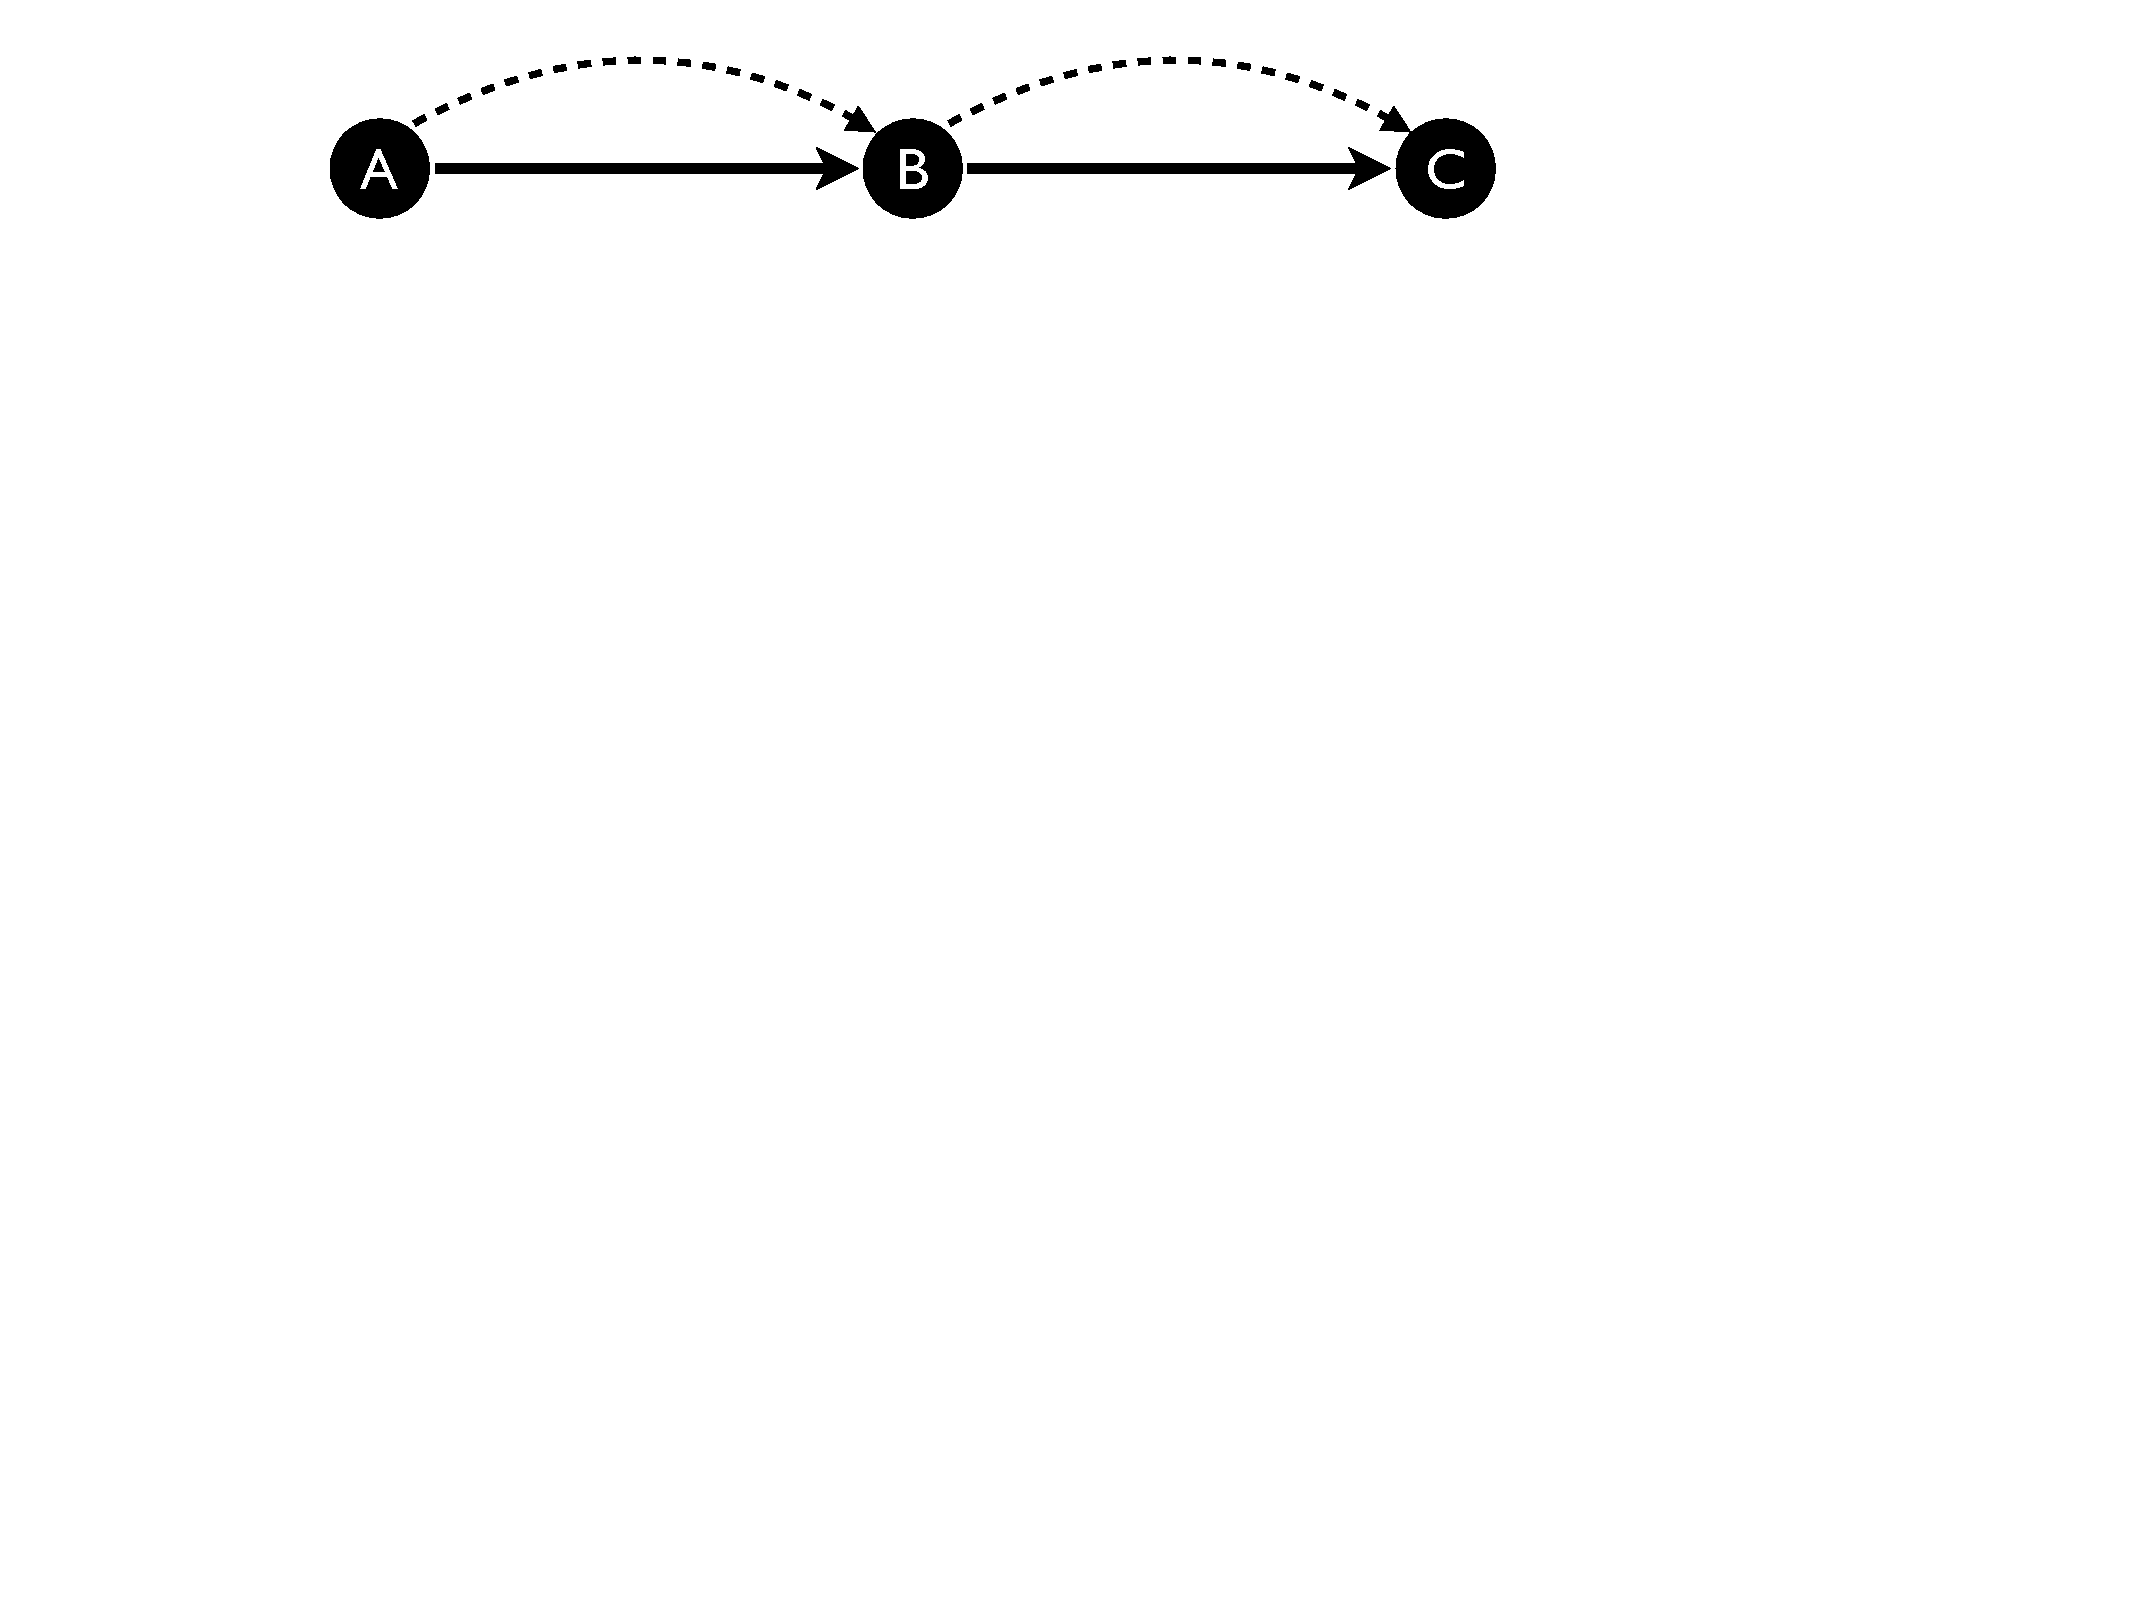
\includegraphics[width=0.5\columnwidth]{figs/seg1}}
  \subfigure[
  Old path: $A \rightarrow B \rightarrow 2 \rightarrow C$, new path: $A \rightarrow 2 \rightarrow B \rightarrow C$. 
  New $AB$ crosses old $BC$, so $AB$ depends on $BC$]{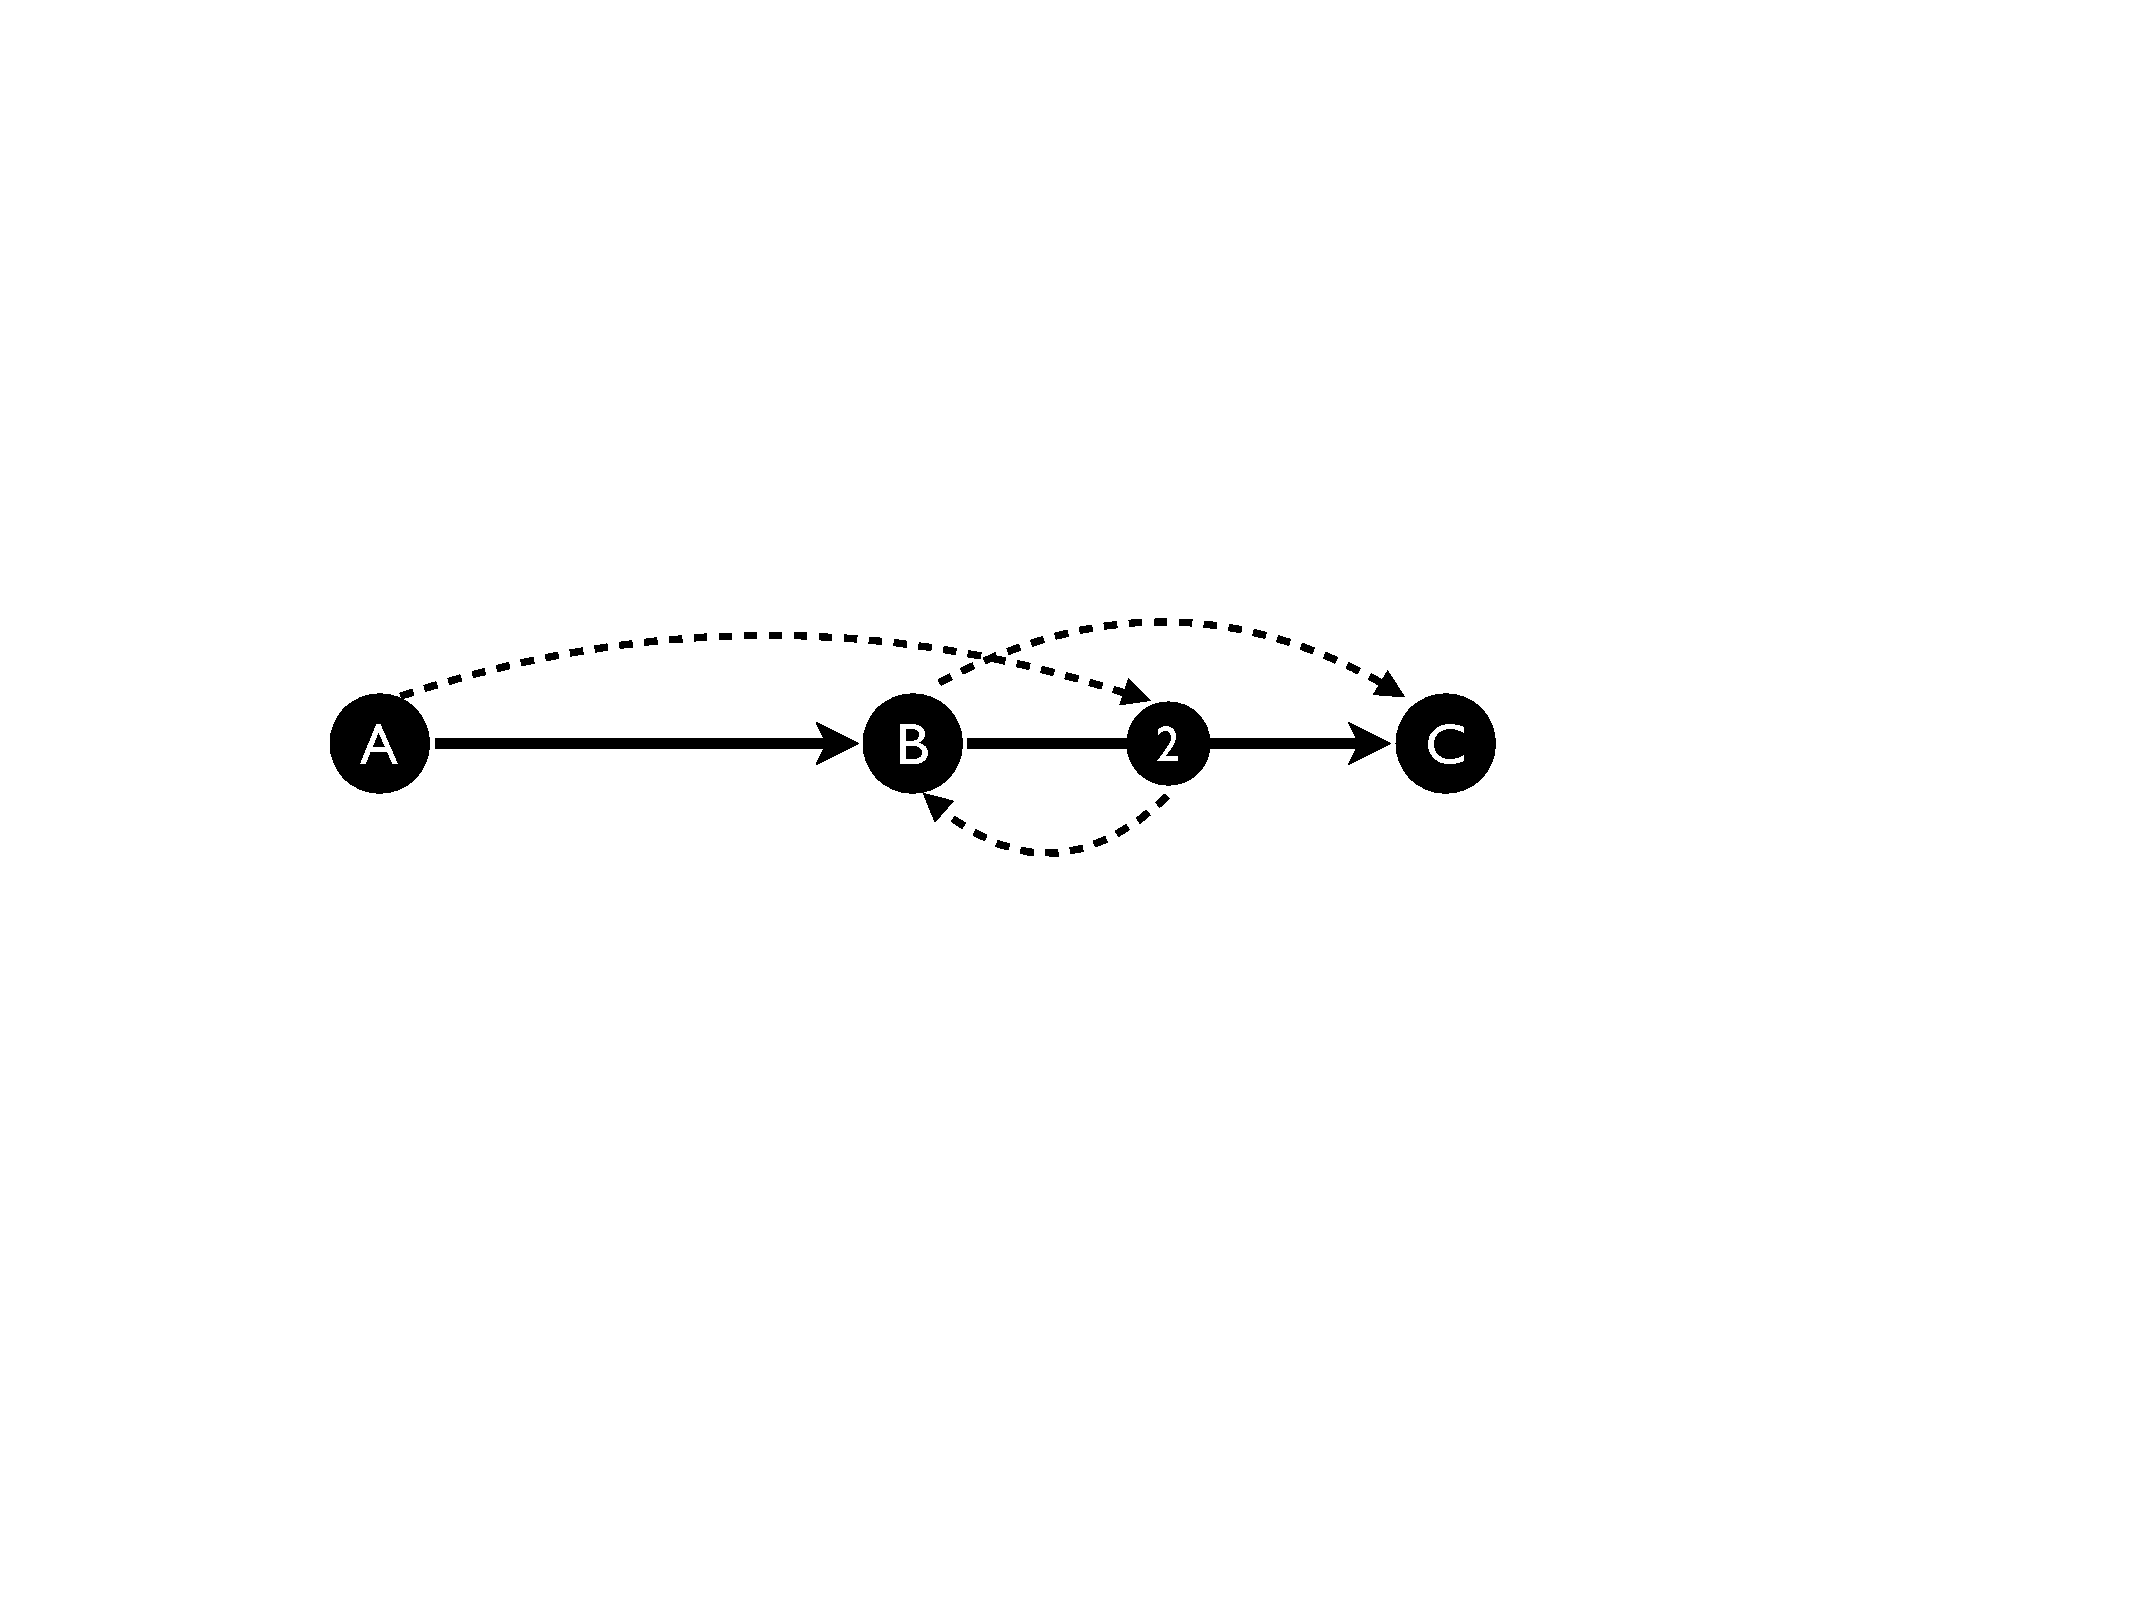
\includegraphics[width=0.5\columnwidth]{figs/seg3}}
  \subfigure[
  Old path: $A \rightarrow 1 \rightarrow B \rightarrow C$, new path: $A \rightarrow B \rightarrow 1 \rightarrow C$. 
  New $BC$ crosses old $AB$, so $BC$ depends on $AB$]{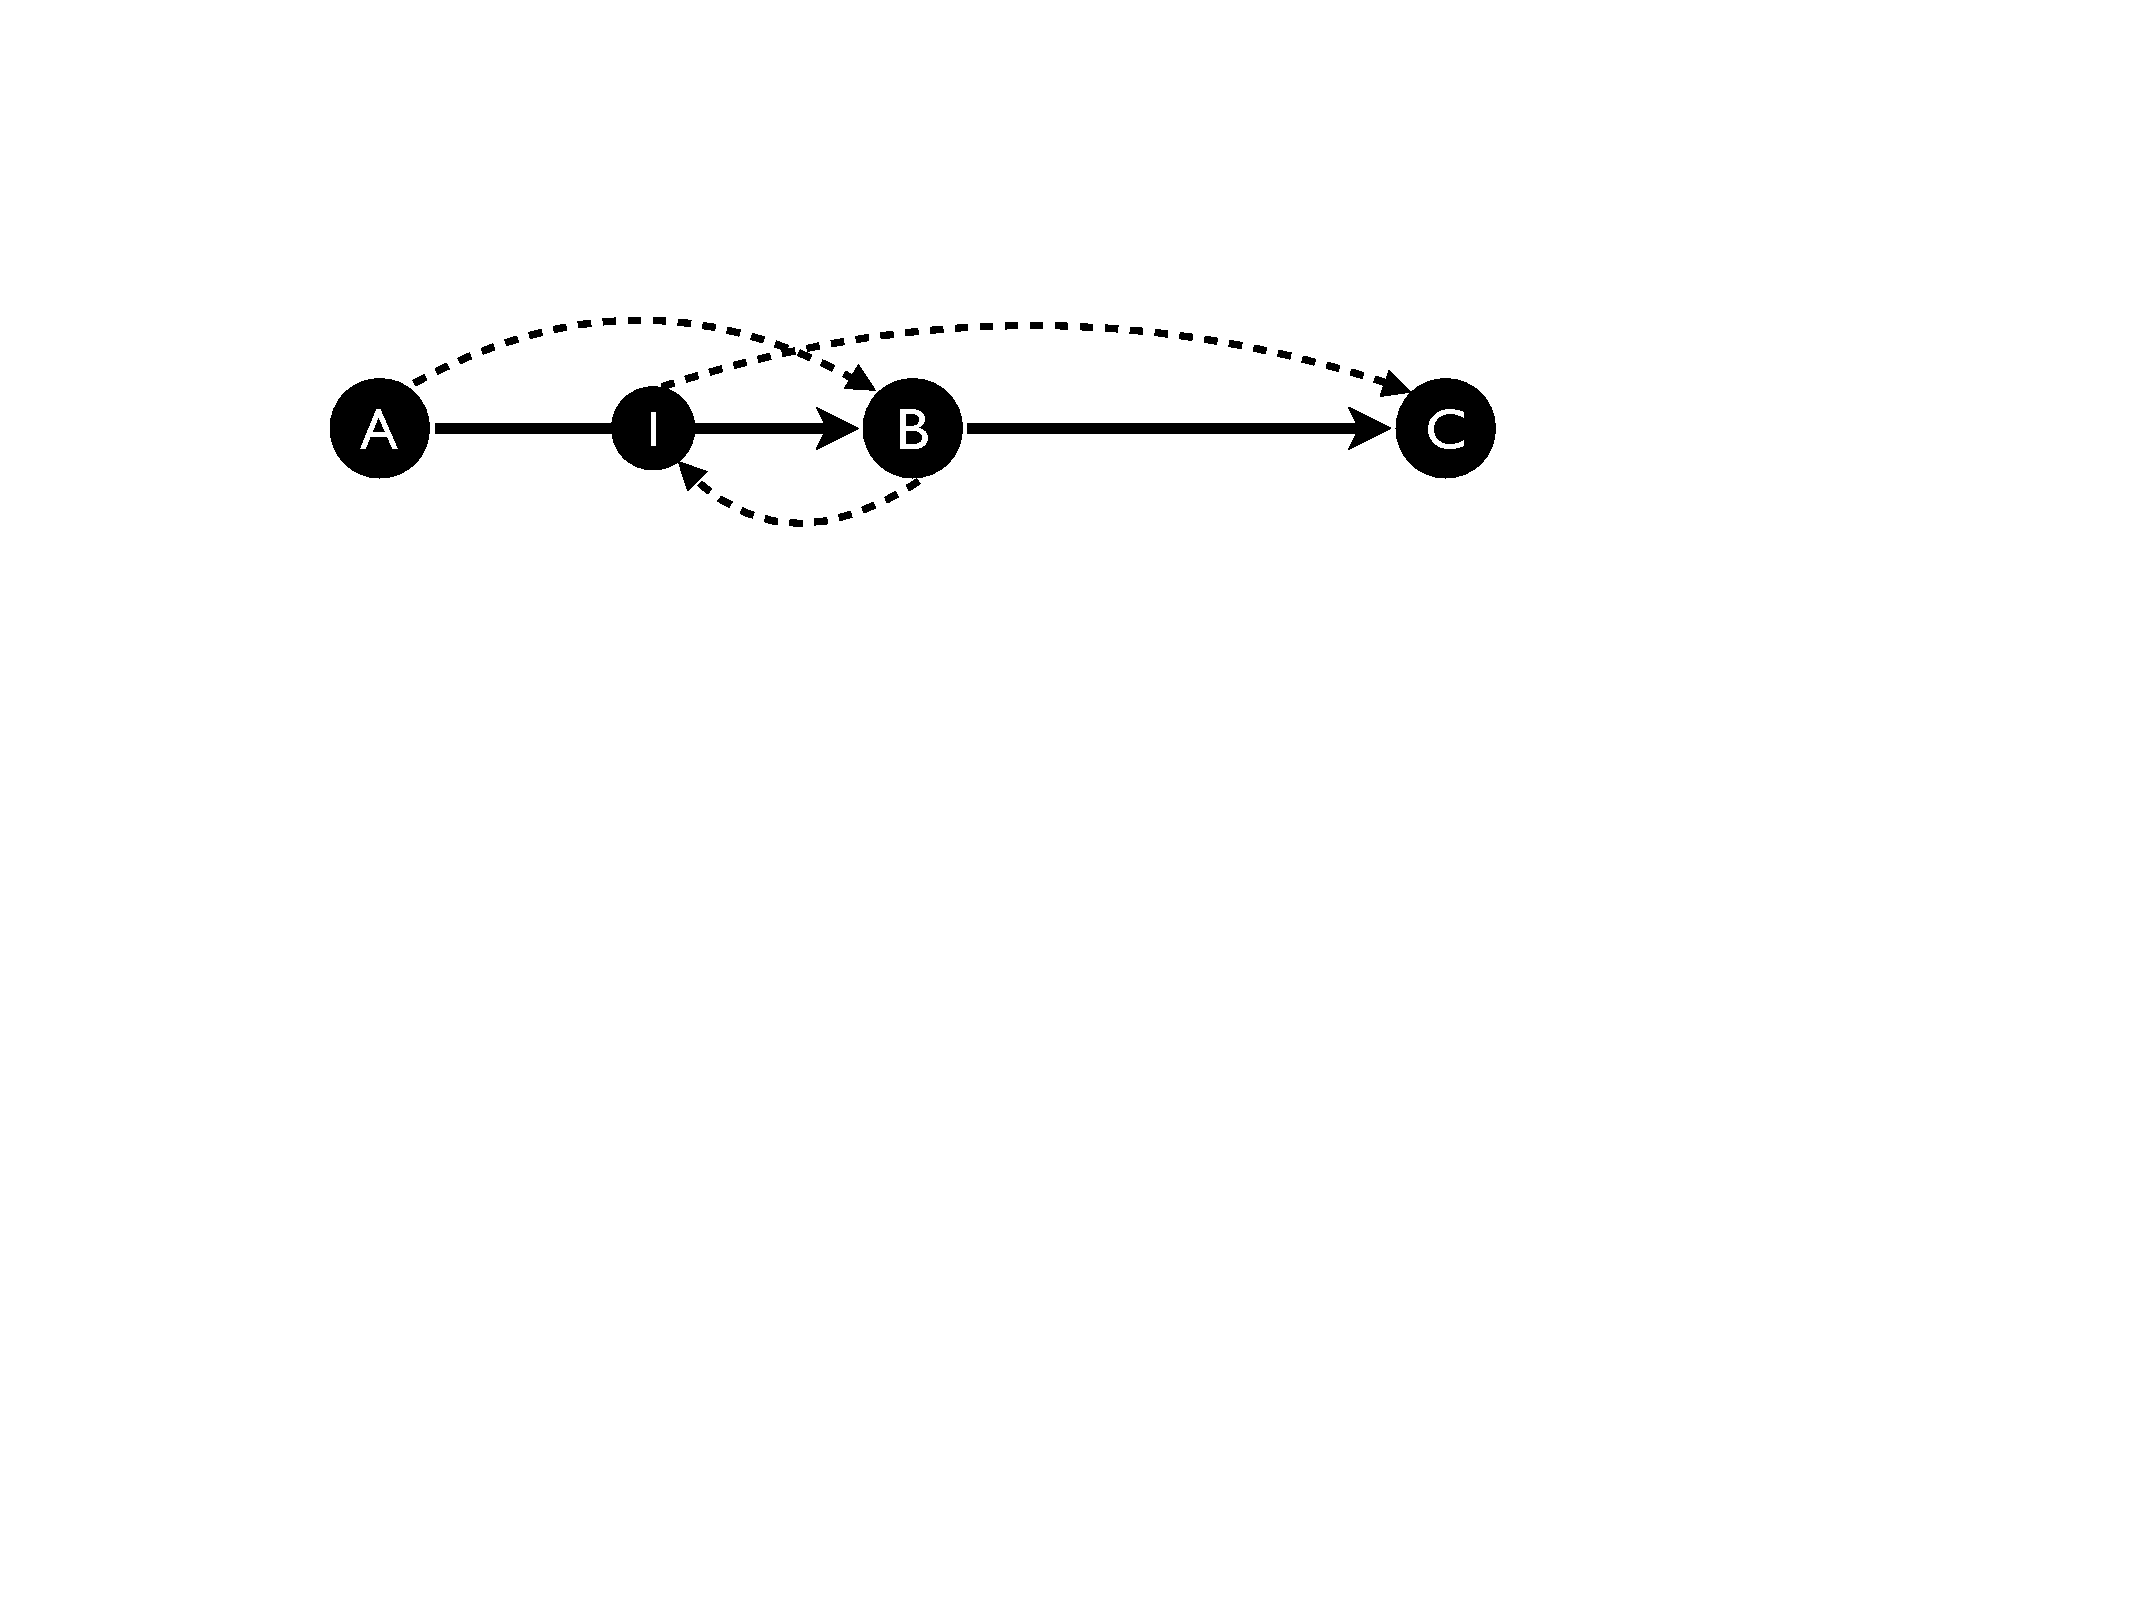
\includegraphics[width=0.5\columnwidth]{figs/seg2}}
  \subfigure[
  Old path: $A \rightarrow \rightarrow 1 \rightarrow B \rightarrow 2 \rightarrow C$, new path: $A \rightarrow 2 \rightarrow B \rightarrow 1 \rightarrow C$. 
  New $BC$ crosses old $AB$, and new $AB$ crosses old $BC$, so $BC$ and $AB$ have circular dependency between themselves.]{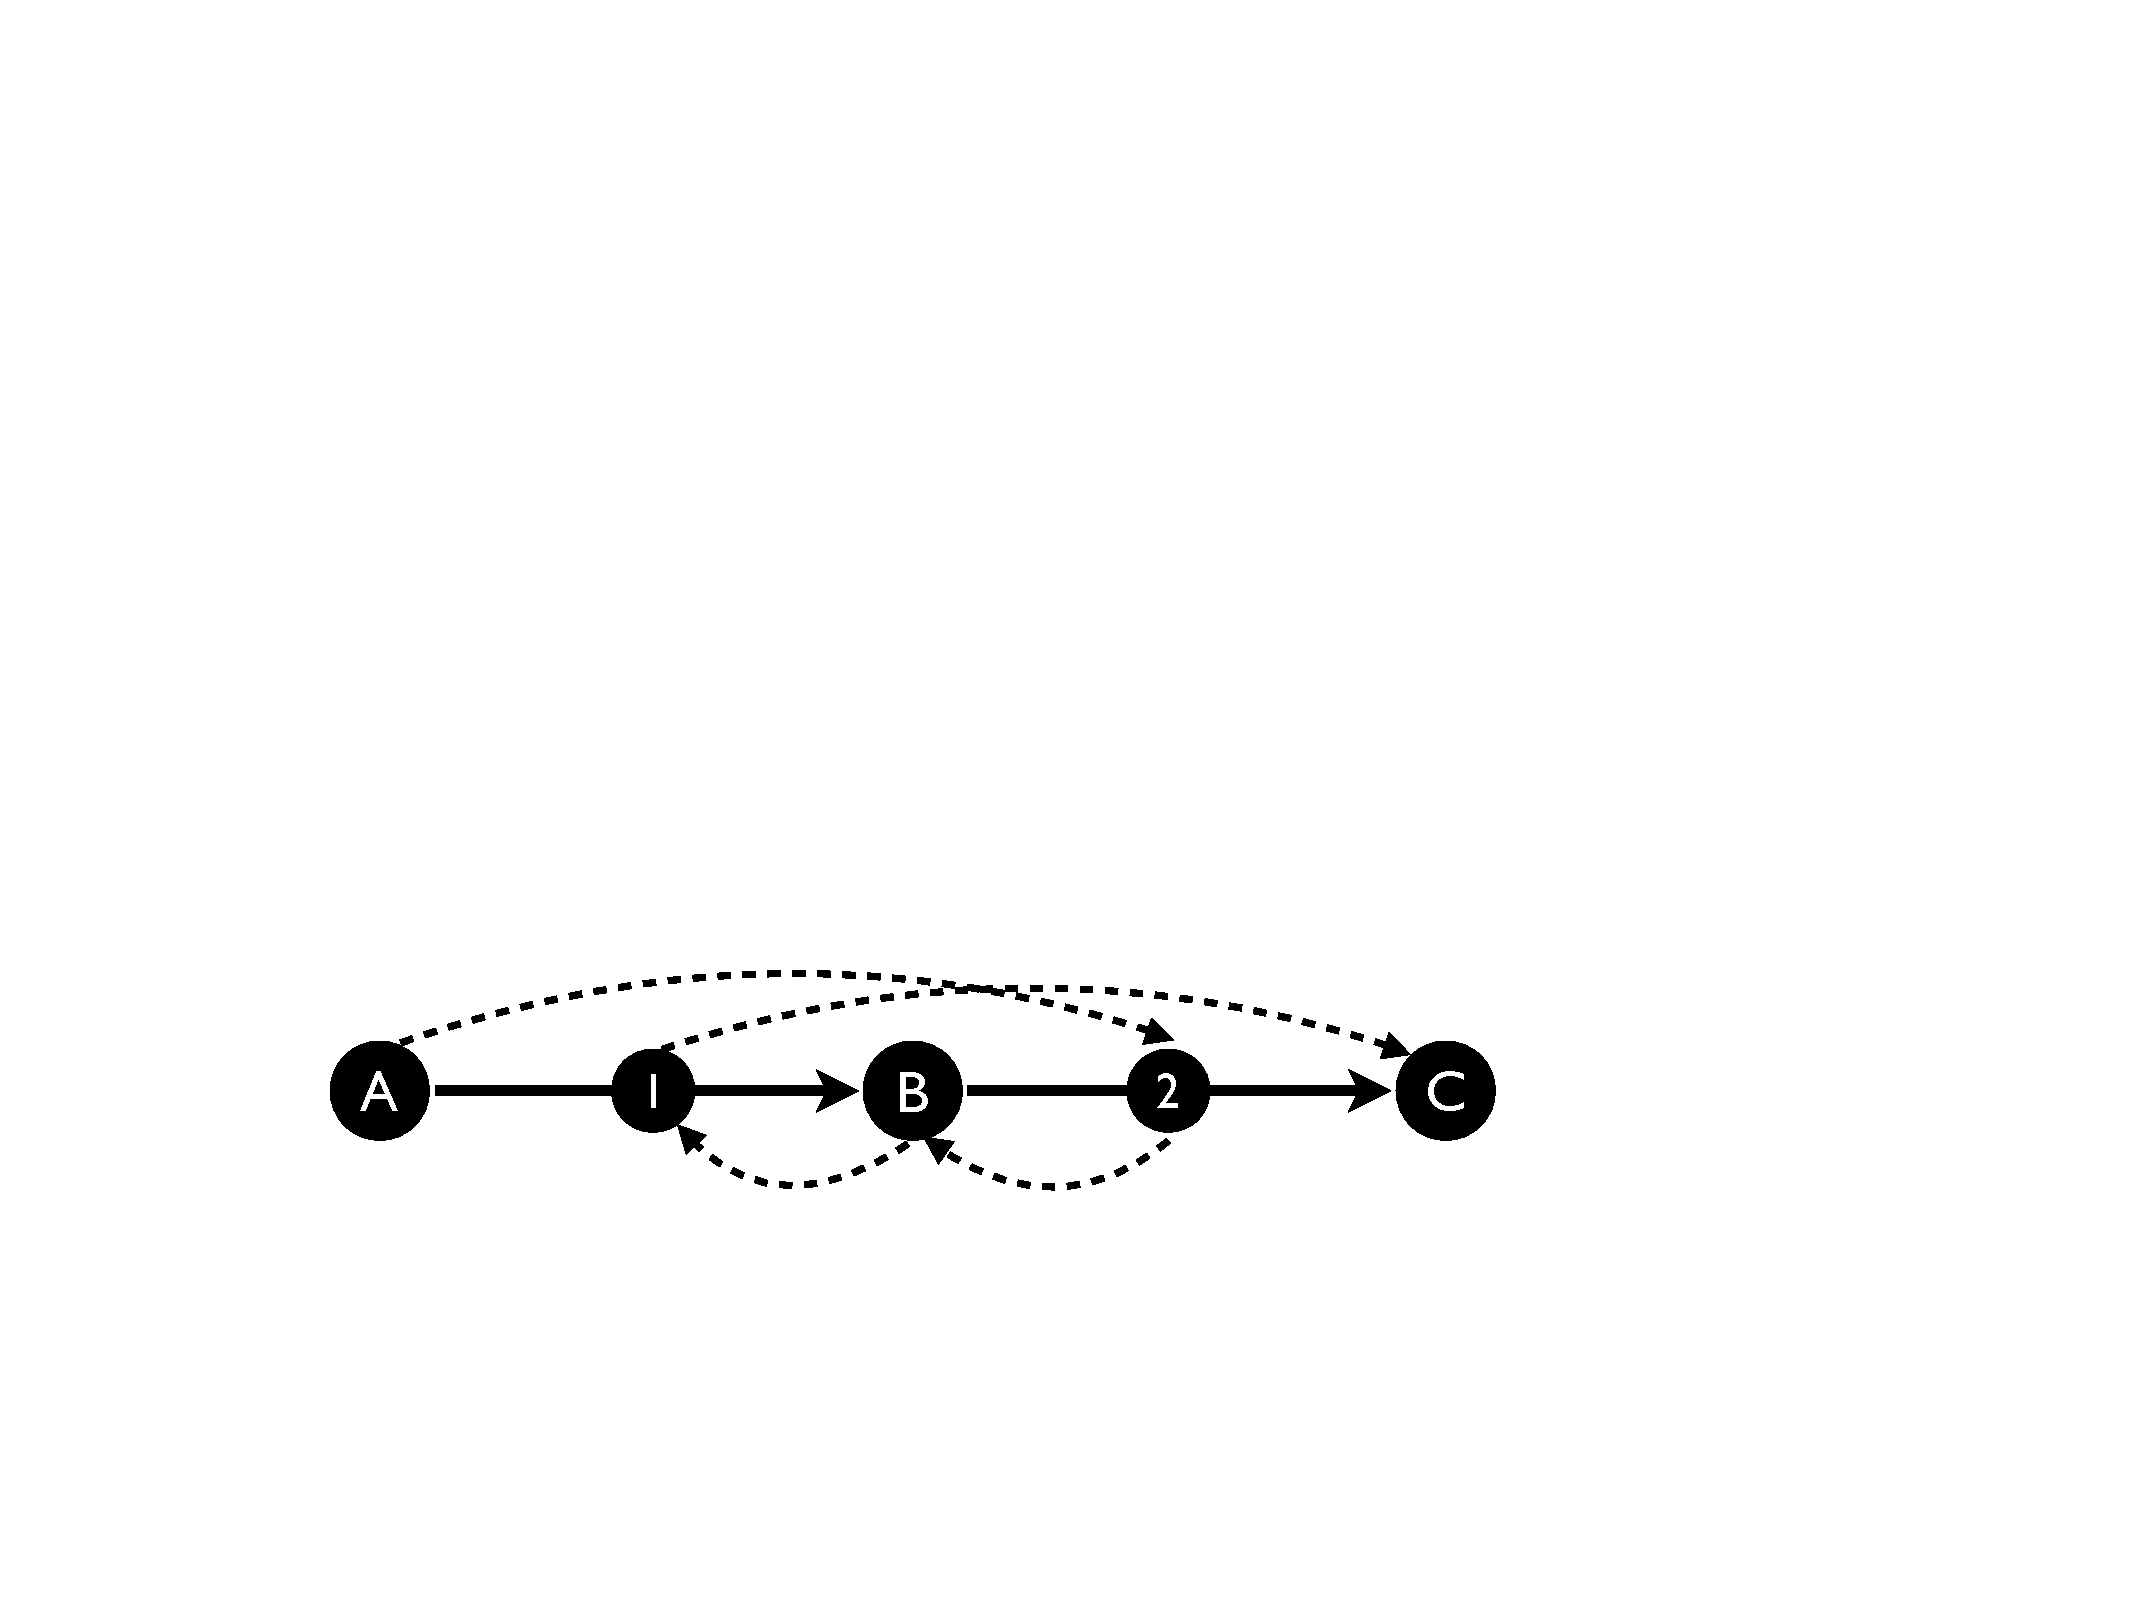
\includegraphics[width=0.5\columnwidth]{figs/seg4}}
  %\subfigure[case 5]{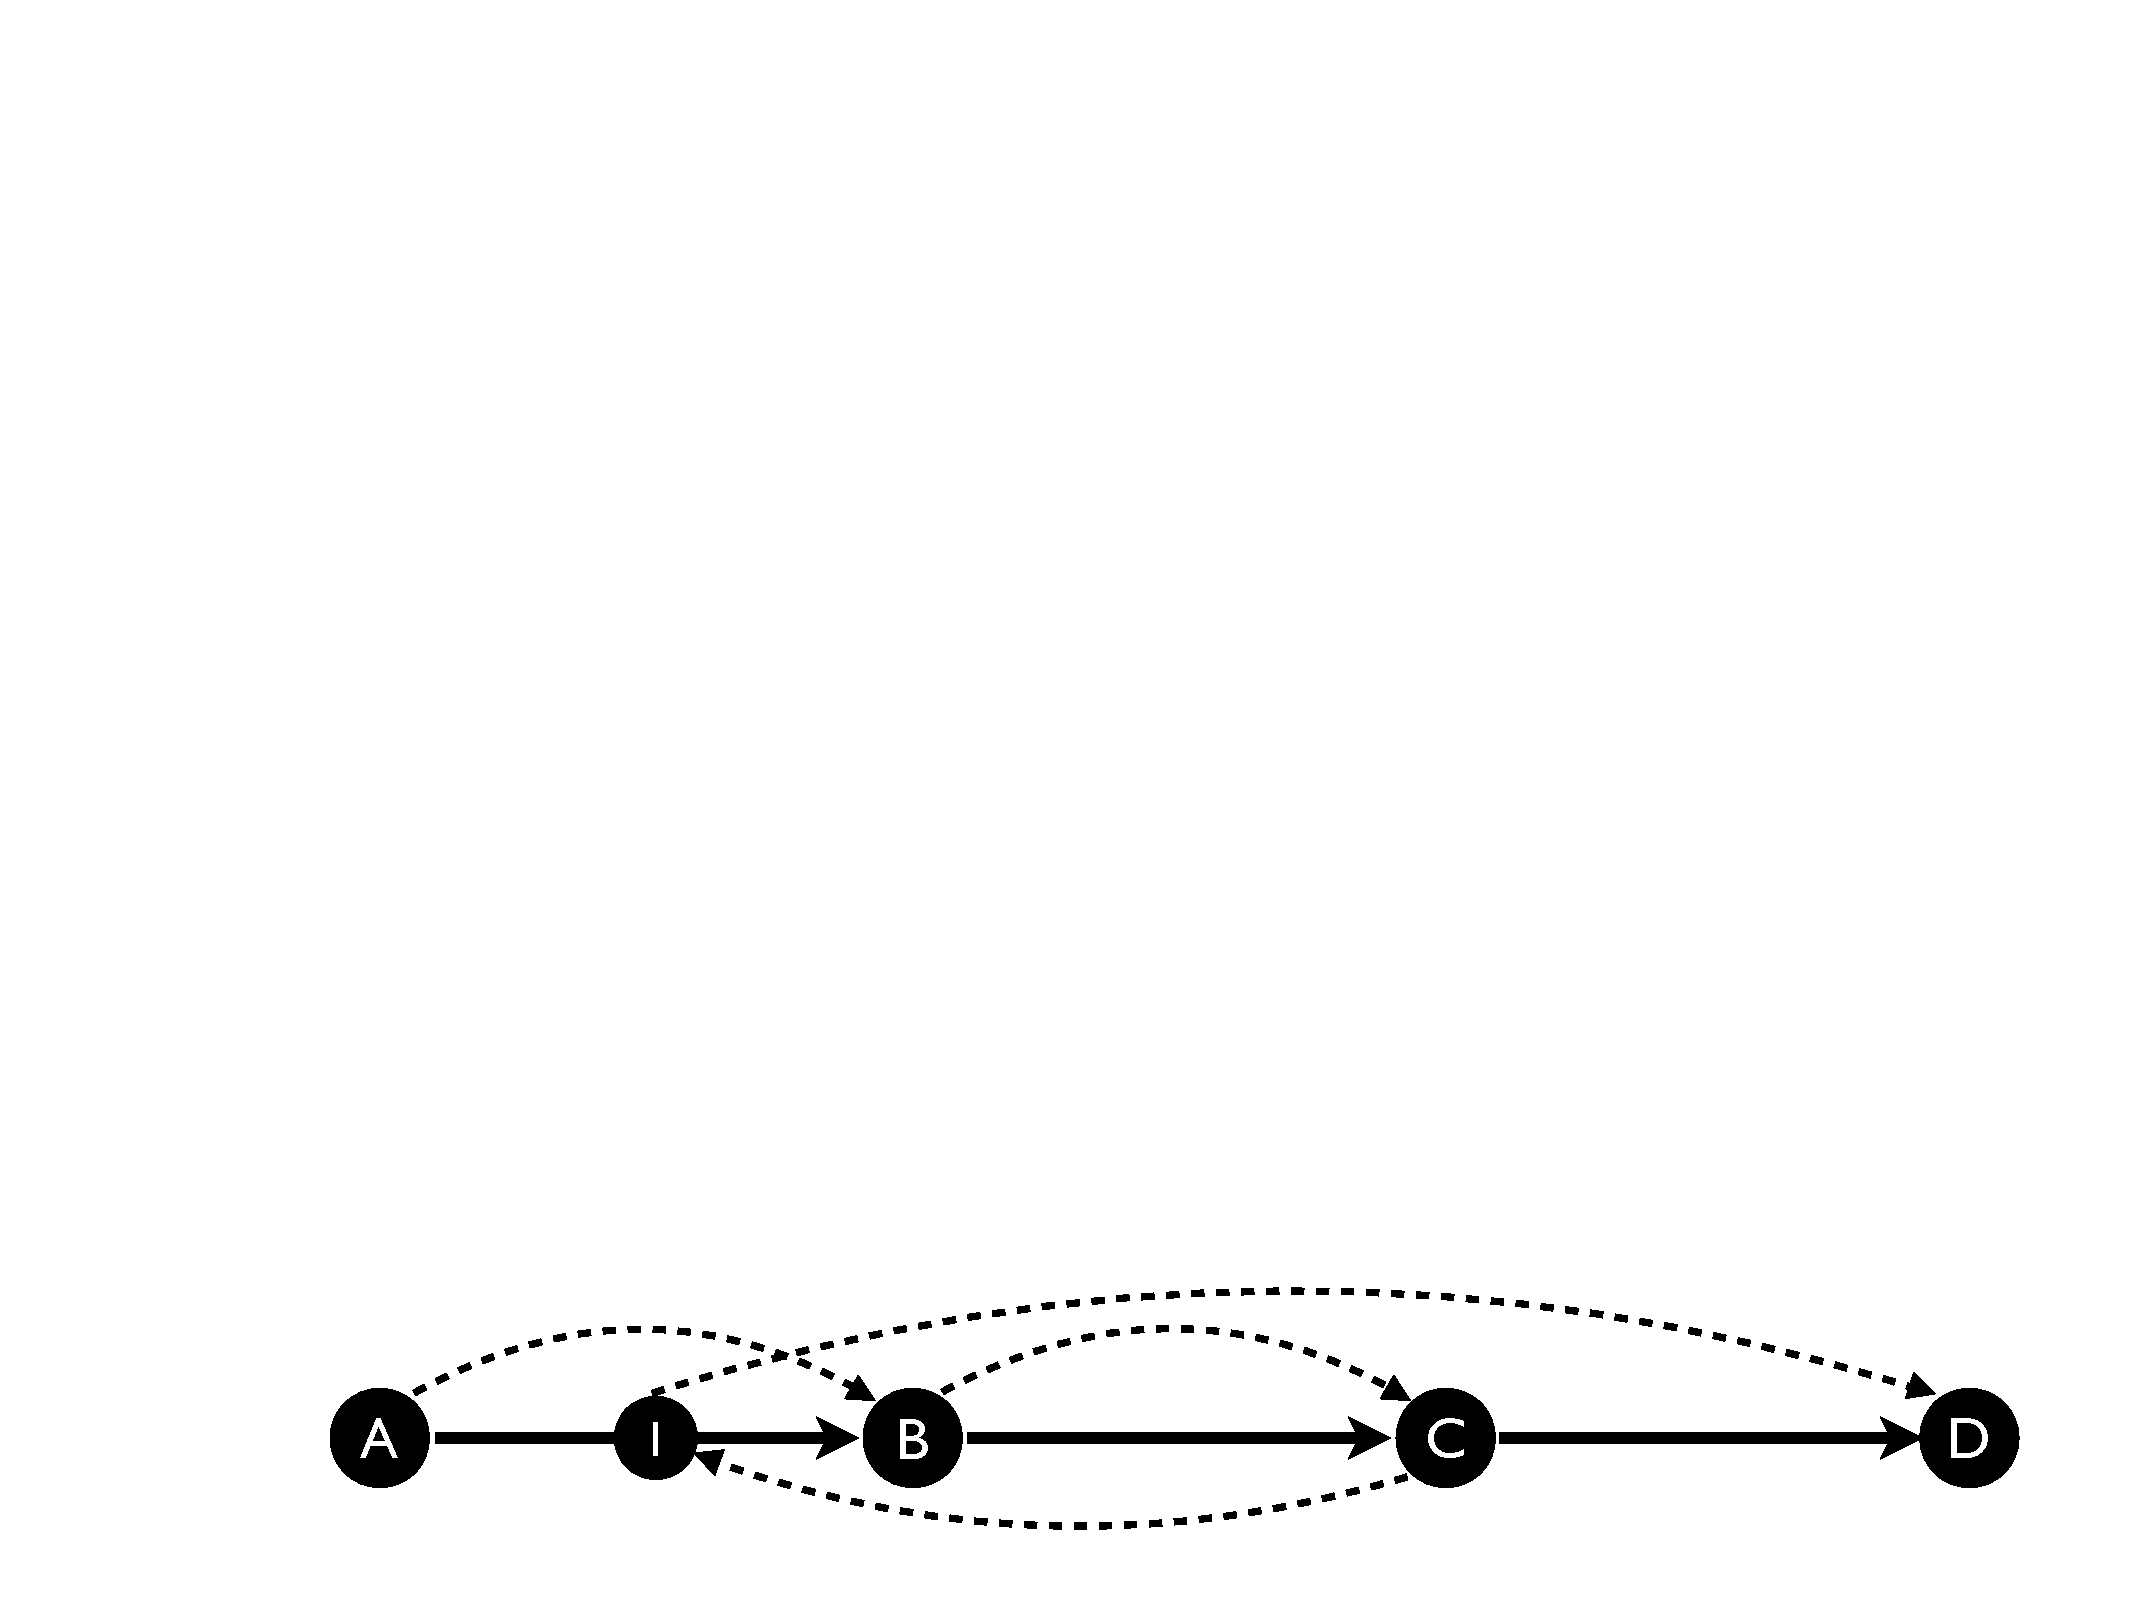
\includegraphics[width=0.7\columnwidth]{figs/seg5}}
  %\vspace{10pt}
  \vspace{-0.2in}
  \caption{\em \small Examples: dependencies between segments. Path $AC$ is divided into two segments $AB$ and $BC$ by three waypoints $A$, $B$, and $C$, with old paths in solid lines, and new paths in dashed lines. \kevinc{changes in the subtitle to clearly specify the new/old path} }
  \vspace{-0.2in}
  \label{fig:circular}
\end{figure*}

  \vspace{-0.1in}
\begin{theorem} If there is no circular dependency between segments, then an update order that preserves the required property always exists. 
In particular, if policies are enforcing no more than two waypoints,
an update order always exists. 
%\begin{itemize}[noitemsep,topsep=0pt,leftmargin=*]
%\item independent ECs, i.e., no overlapping updates across different ECs.
%\item no circular dependencies between segments. 
%In particular, if invariants are enforcing no more than two waypoints.
%an update order always exists. 
%\end{itemize} 
\end{theorem}
  \vspace{-0.1in}

If a policy introduces no circular dependency, 
i.e., at least one segment can be updated independently (Figure~\ref{fig:circular}(a-c)), 
then we say the policy is {\em segment independent}.
%Figure~\ref{fig:circular}(a) shows us one such example. 
However, in reality, forwarding links and paths may be shared by different sets of packets, e.g., multiple flows. Thus it is possible that two forwarding links (smallest possible segments) $l_1$ and $l_2$ will have 
conflicting dependencies when serving different groups of packets, e.g., in forwarding graphs destined to two different IP prefixes. In such cases, circular dependencies are formed across forwarding graphs. 
Fortunately, forwarding graphs do not share links in many cases. 
For example, as pointed out in~\cite{jin2014dynamic}, a number of flow-based traffic management applications 
for the network core (e.g., ElasticTree, MicroTE, B4, SWAN~\cite{microte, heller2010elastictree, jain2013b4, Hong13}), any forwarding rule at a switch matches at most one flow.

%\wxzc{need to prove it holds for multi-path?}

\paragraph{Other Properties}

There are trace properties which are not waypoint-based, such as
quantitative properties like path length constraint. 
To preserve such properties and waypoint-based trace properties that are not segment independent,
\kevin{we can use other heavyweight techniques as a fallback (see \ref{sec:synthesis}), such as CU~\cite{Reitblatt2012}.}
%\name is plugged in with CU~\cite{Reitblatt2012} as backup to its heuristic component. 
Besides, there are network properties beyond trace properties, such as congestion freedom,
%\cut{quality of service, and }congestion freedom. 
%Among those, congestion freedom is a common and important one. 
and it has been proven that careful ordering of updates cannot always guarantee congestion freedom~\cite{Hong13, loopfree-flow}. 
\kevin{To ensure congestion freedom, one approach is to use other heavyweight tools, such as SWAN~\cite{Hong13}, as a fallback mechanism that the default heuristic algorithm can trigger only when necessary.}

%we plug in a heavyweight tool (e.g., SWAN, which is the one used in our implementation) to work together with the heuristic algorithm.  

%Overlapping ECs:
%1. split updates to non-overlapping; 2. use mechanisms like CU.

%Slice isolation: If the output
%of packet set of slice $a$ at any switch port, overlaps with any other slice,
%then there is the potential for leaks. 
%
%Multiple waypoints 

%Path length constraint: Suppose
%we wish to ensure that no flow from port $C$ to port $S$ should go through more
%than 3 switches represents this check.
%
%Quantitative properties (with SWAN)                         

\subsection{Consistency Preserving Network Synthesis}
\label{sec:synthesis}

\wxznew{ 
%\cut{As discussed previously, there may be situations in which this
%greedy algorithm gets stuck, i.e., some buffered updates never pass the
%verification.  That may happen }
When desired policies do not have the segment-independence property (\S\ref{sec:seg-independence}), it is possible that some buffered updates (through very rare in practice) never pass the verification.}
%\cut{ using the greedy algorithm}
For instance, consider a circular network with three nodes, in which each node
has two types of rules: one type to forward packets to destinations directly connected to itself, and one default rule, which covers destinations connected to the other two switches. 
Initially, default rules point clockwise. They later change to
point counter clockwise. No matter which of the new default
rules changes first, a loop is immediately caused for some destination. 
\wxzcr{The loop freedom property is not segment-independent in this case, because that each default rule
is shared by two flows (destined to two hosts),
which results in conflicting dependencies among forwarding links.}
To handle scenarios like that, 
we adopt a hybrid approach (Algorithm 2).  If the network
operators desire some policies that can be guaranteed by existing
solutions, e.g., CU or SWAN, such solutions can be specified and plugged in as
the fallback mechanism, $FB$.
The stream of updates is first handled by \name's greedy heuristic (Algorithm 1)
%from the application is first fed into the translation layer to be transformed
%to a feasible update sequence. Then \name greedily sends updates
as long as the
policy is preserved. Updates that violate the policy are buffered temporarily.
When the buffering time is over threshold $T$, configured by the operator,
the fallback mechanism is triggered.
The remaining updates are fed into $FB$ to be transformed to a feasible sequence, and then Algorithm 1 proceeds with them again to heuristically maximize update parallelism. 
In that way, \name can always generate a consistent update sequence.
%\cut{avoids getting stuck.}
Alternatively, if no such external mechanism exists, 
\kevinc{prefer to remove ``if no such external mechanism exists"} or the operators highly
value update efficiency and prefer a best effort mechanism to maintain consistency
during updates, no fallback would be triggered and no
$FB$ would be provided to the algorithm.  Instead, after a
configurable threshold of time, buffered commands are released to the network.
\wxzcr{Thus, all updates are guaranteed to be issued eventually either way.}
%Such design gives operators a flexible choice on how to balance the trade-off between efficiency and consistency.
\wxzcr{Note that even with $FB$ triggered, \name achieves better efficiency 
than using $FB$ alone to update the network,
because: 1) in the common case, most of updates are not handled by $FB$;
2) \name only uses $FB$ to "translate" buffered updates and then 
heuristically parallelize issuing the output of $FB$, 
but doesn't wait explicitly as some $FB$ mechanism does, e.g., the waiting time between two phases in CU.}

%  \vspace{-0.1in}
\begin{algorithm}[t]
  \small
\caption{Synthesizing update orderings}
\bf{ScheduleUpdates}($Model, Buf, U, FB, T$)
\begin{algorithmic} 
\For {$u \in U$}
        \State \bf{ScheduleIndividualUpdate($Model, Buf, u$)}
\EndFor
\State 
\State \bf{On timeout($T$):}
\State $\tilde{U}$ = \bf{Translate($Buf, FB$)}
\For {$u \in \tilde{U}$}
        \State \bf{ScheduleIndividualUpdate($Model, Buf, u$)}
\EndFor
\label{alg:synthesize}
\end{algorithmic}  
\end{algorithm}

\if 0
\begin{figure}[!ht]
  \centering
  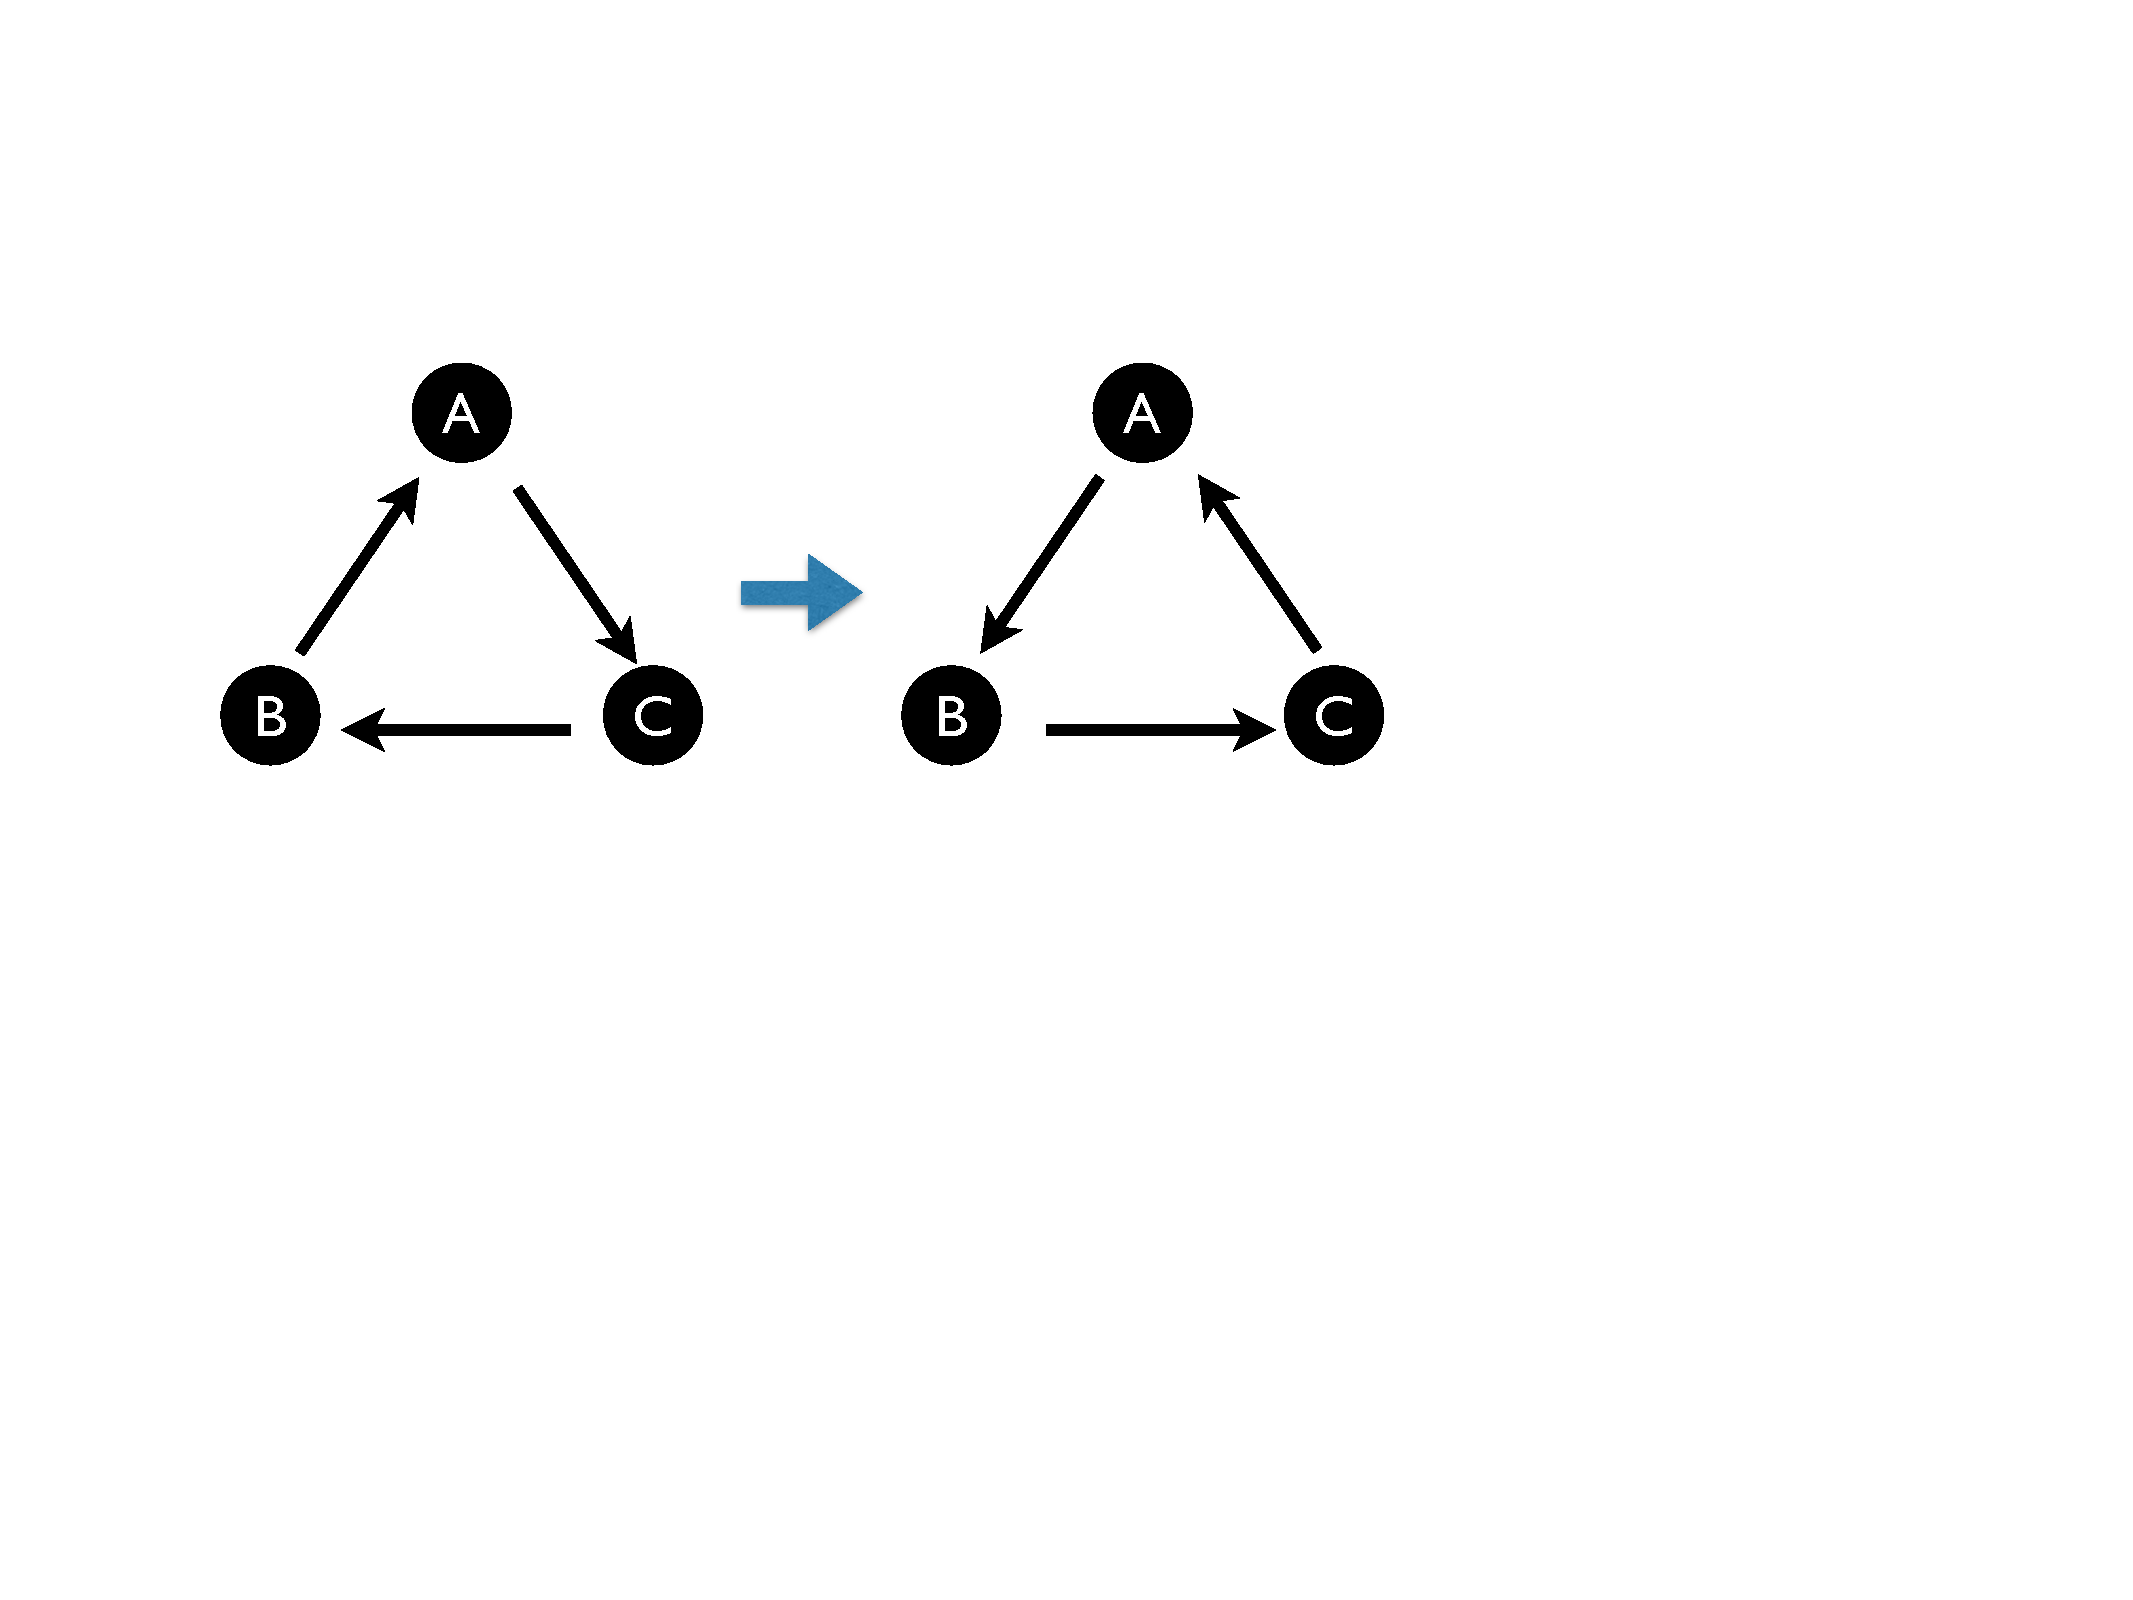
\includegraphics[width=0.7\columnwidth]{figs/triangle}
  \caption{\em \small Illustrating case where Algorithm1 gets stuck.}
  \label{fig:example}
\end{figure}
\fi

To show the feasibility of that approach,
%\cut{we integrated \name with both CU \cite{Reitblatt2012} and SWAN \cite{Hong13} as plug-ins.} 
\kevin{we implemented both CU \cite{Reitblatt2012} (see \S\ref{sec:eval}) and SWAN \cite{Hong13} as our fallback mechanisms in \name.}
%\cut{The integration with CU is thoroughly evaluated in \S\ref{sec:eval}, and here, we focus on the one with SWAN. } 
%We verified congestion-free invariants of 
We emulated traffic engineering (TE) and failure recovery (FR), similar to Dionysus \cite{jin2014dynamic}, in the network shown in Figure \ref{fig:swan_topo}. Network updates were synthesized to preserve congestion-free property using \name (with SWAN as plug-in), and for comparison, using SWAN alone. In the TE case, we changed the network traffic to trigger new routing updates to match the traffic. In the FR case, we turned down the link S3-S8 so that link S1-S8 was overloaded. Then the FR application computed new updates to balance the traffic.
 %and eventually eliminate the link overload. 
The detailed events that occurred at all eight switches are depicted in Figure \ref{fig:bw}. We see that \name ensured the same consistency level, but greatly enhanced parallelism, and thus achieved significant speed improvement (1.95x faster in the TE case, and 1.97x faster in the FR case).

\begin{figure}[!ht]
  \centering
  \vspace{-0.1in}
  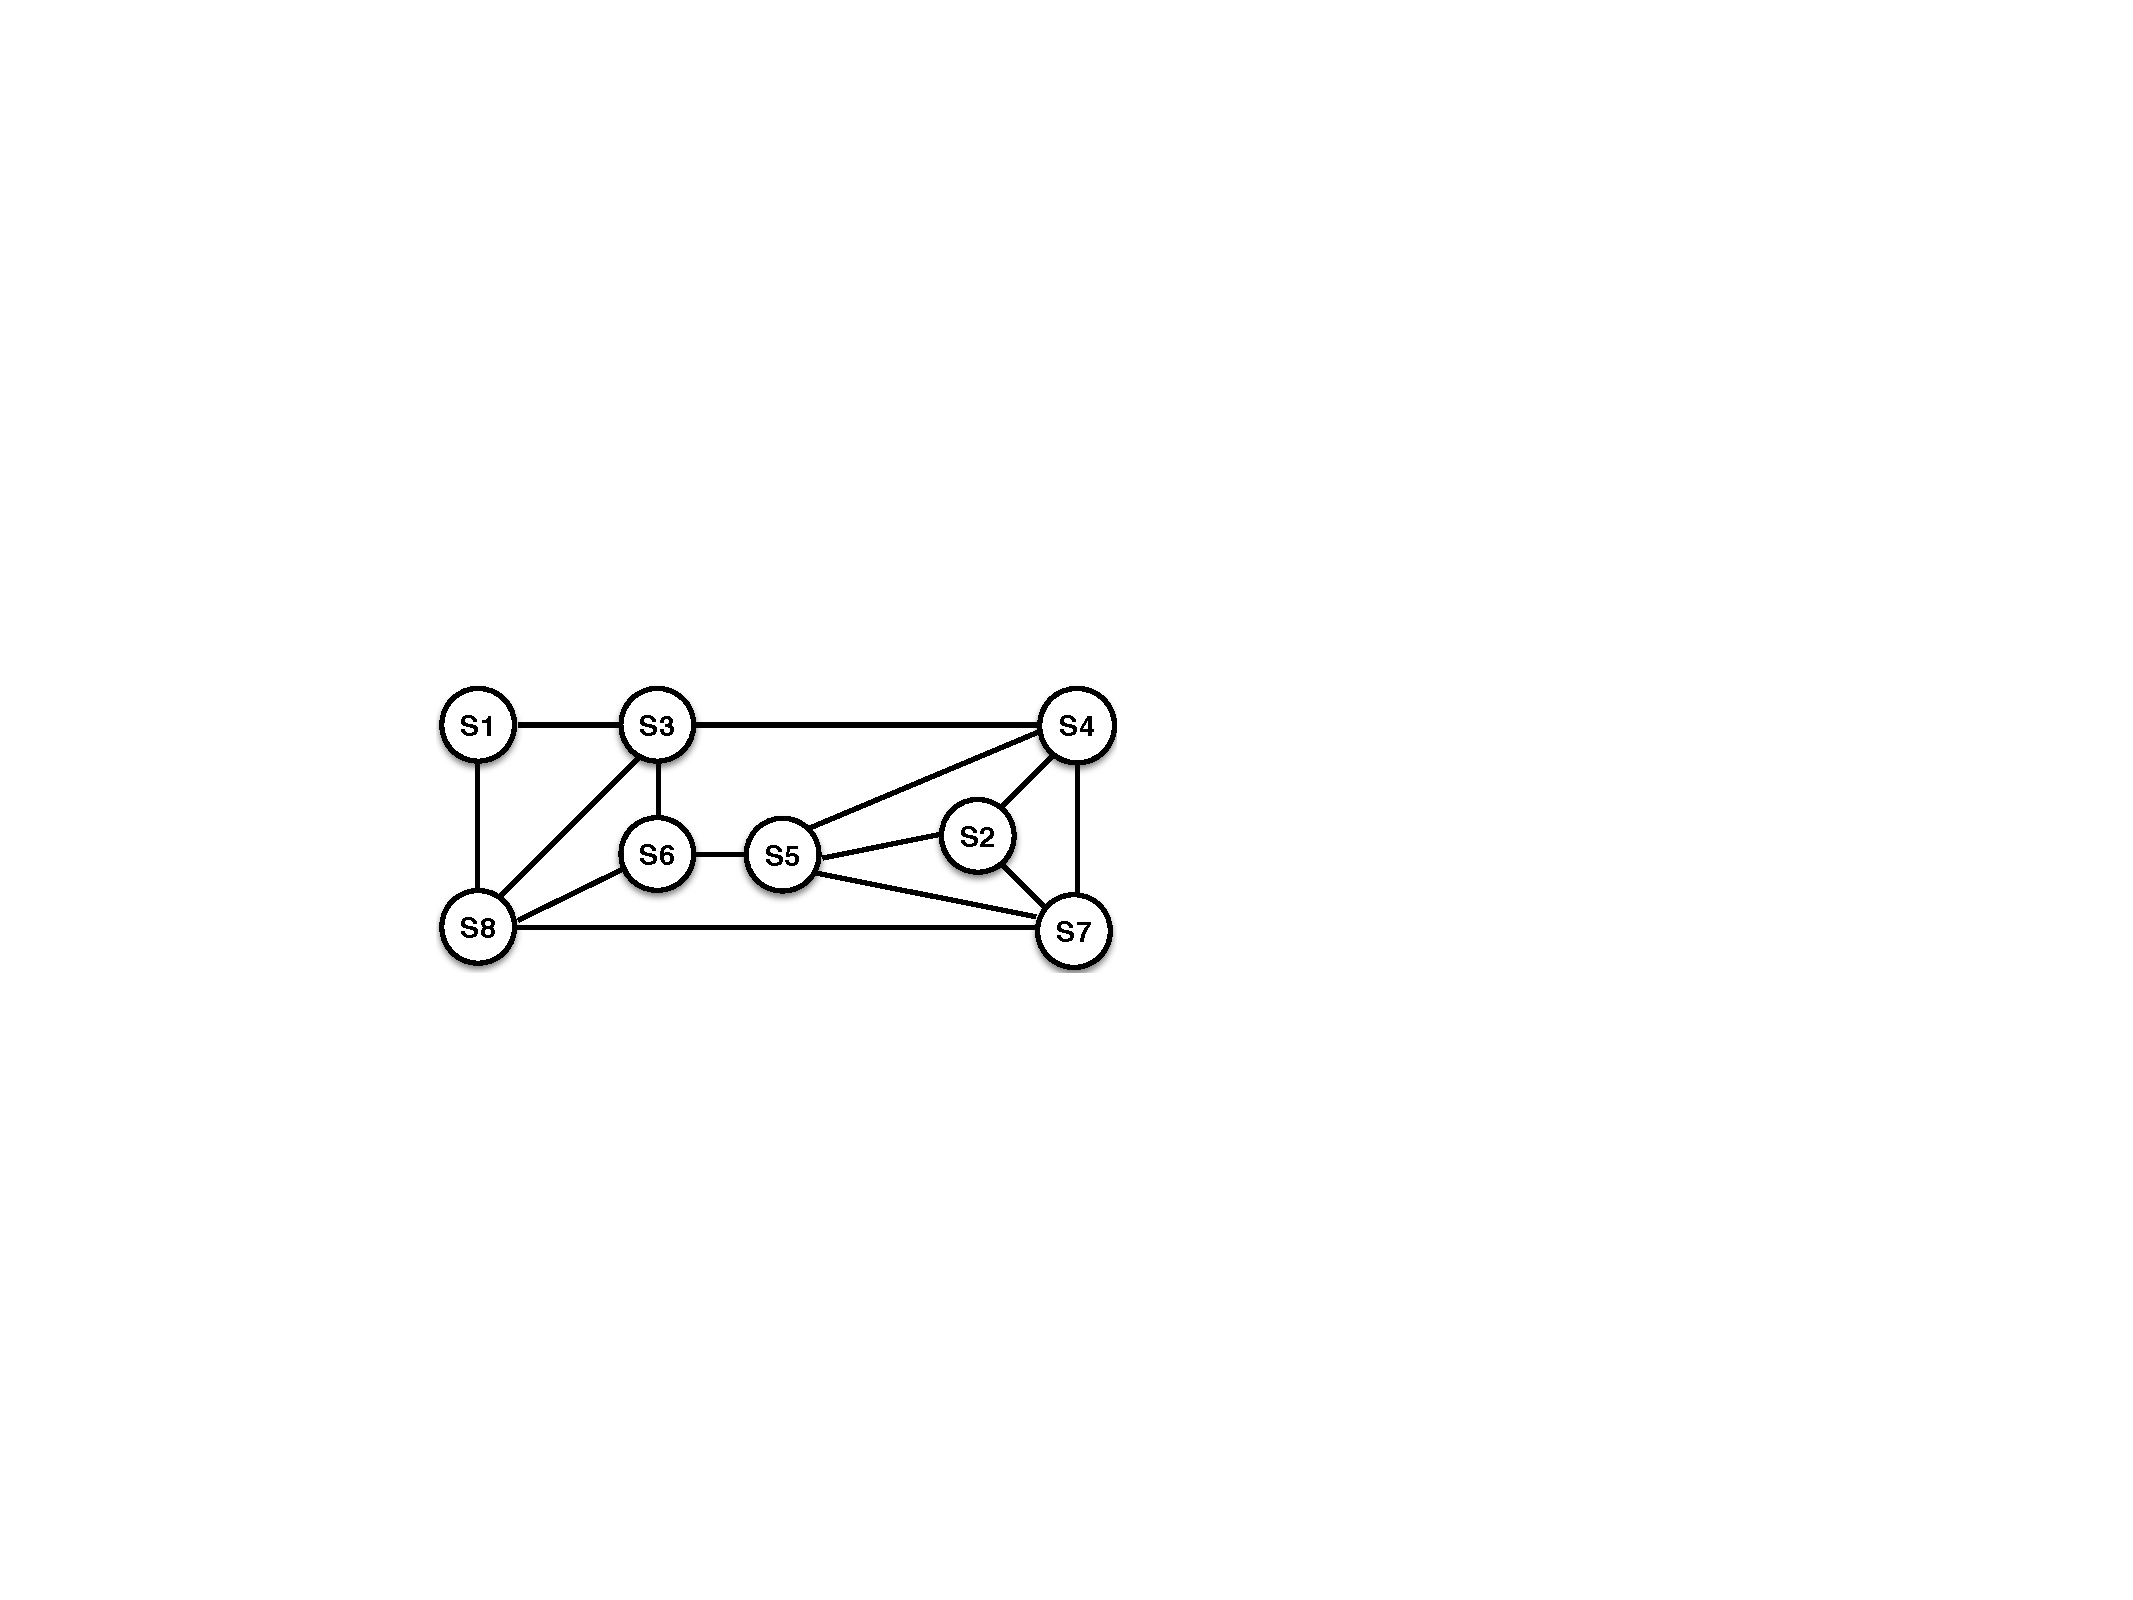
\includegraphics[width=0.5\columnwidth]{figs/swan_topo}
  \vspace{-0.12in}
  \caption{\em \small Topology for \name and SWAN bandwidth tests}
  \vspace{-0.25in}
  \label{fig:swan_topo}
\end{figure}

\cut{
\begin{figure*}[!ht]
  \centering
  \vspace{-0.1in}
  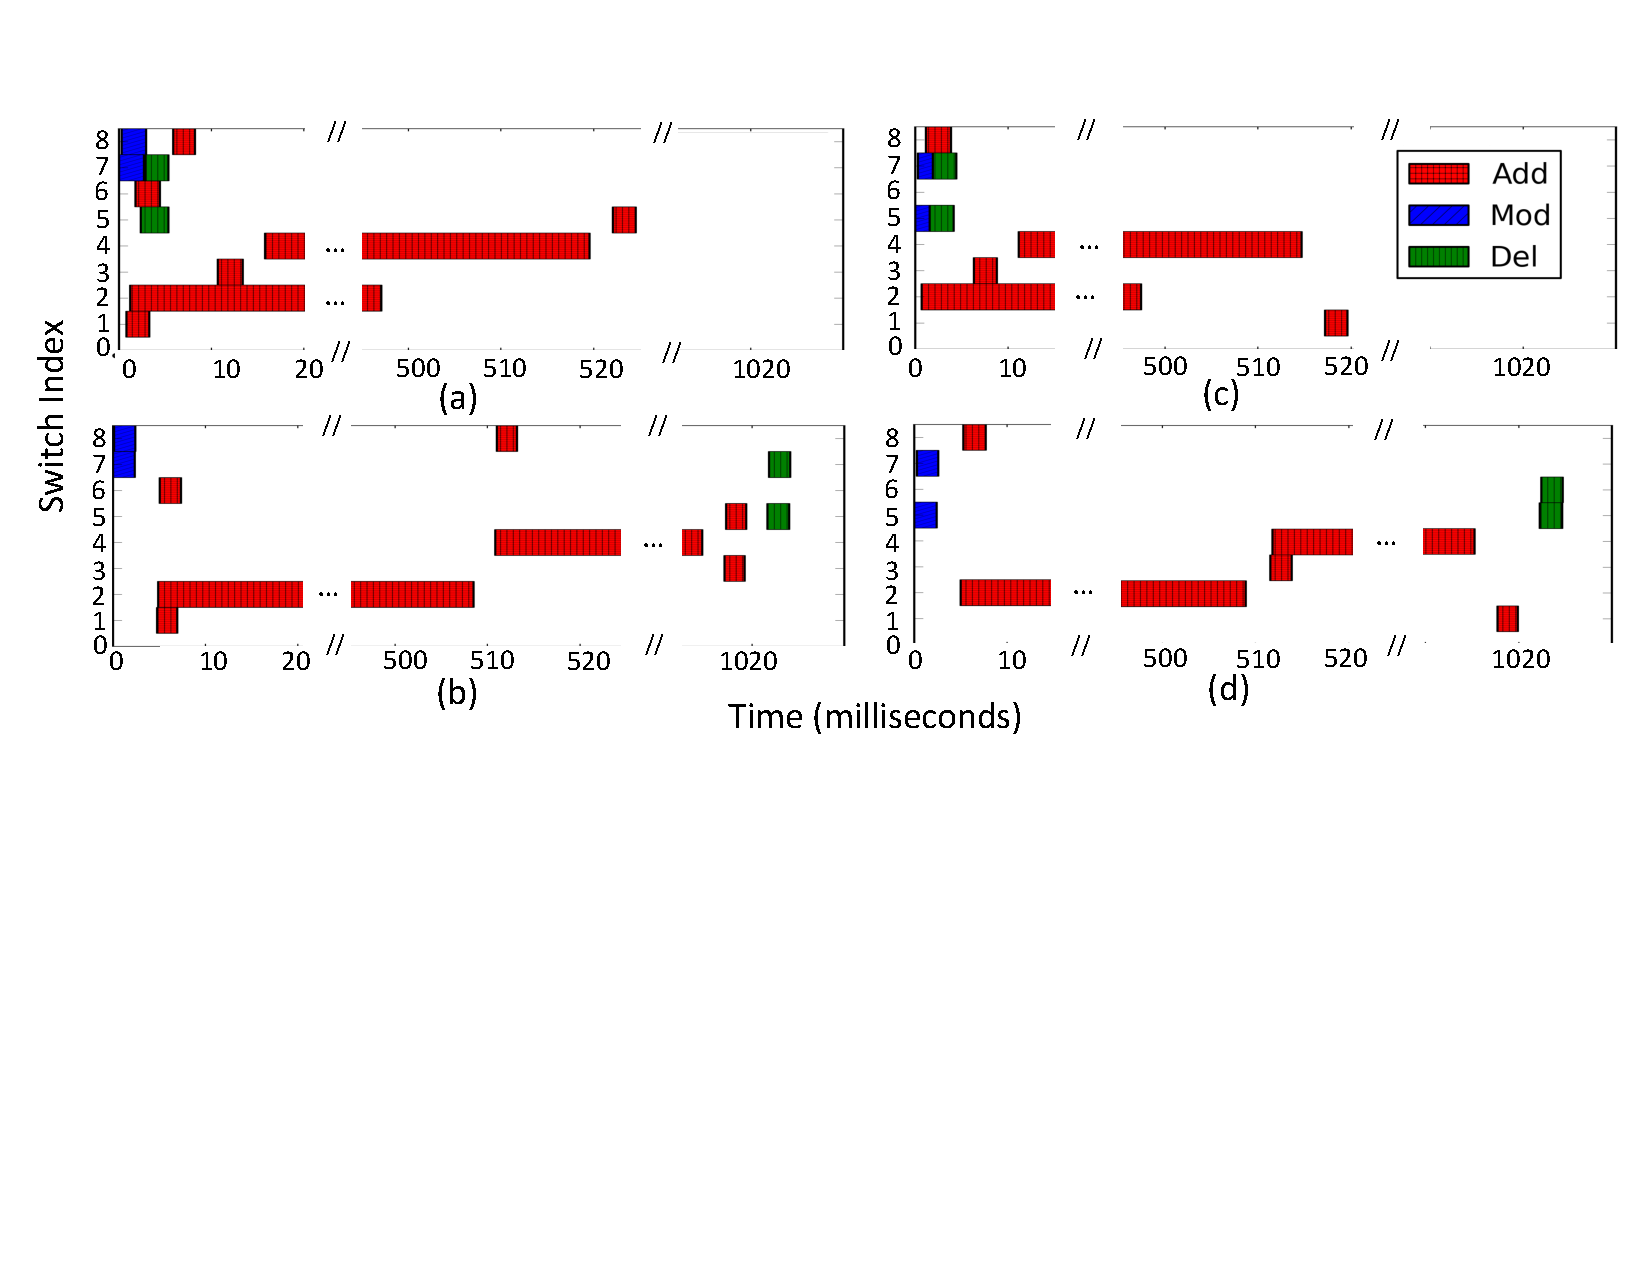
\includegraphics[width=0.8\textwidth]{figs/bandwidth}
  \vspace{-0.1in}
  \caption{\em Time series of events that occurred across all switches: (a) SWAN + \name, traffic engineering; (b) SWAN, traffic engineering; (c) SWAN + \name, failure recovery; (d) SWAN, failure recovery.}
  \vspace{-0.2in}
  \label{fig:bw}
\end{figure*}
}

 \begin{figure*}
        \begin{minipage}[b]{1.2in}
        \caption{\label{fig:bw}\em Time series of events that occurred across all switches: (a) SWAN + \name, traffic engineering; (b) SWAN, traffic engineering; (c) SWAN + \name, failure recovery; (d) SWAN, failure recovery. In both cases, \name + SWAN finishes about 2x faster.}
        \end{minipage}
        \hfill
        \begin{minipage}[b]{6in}
        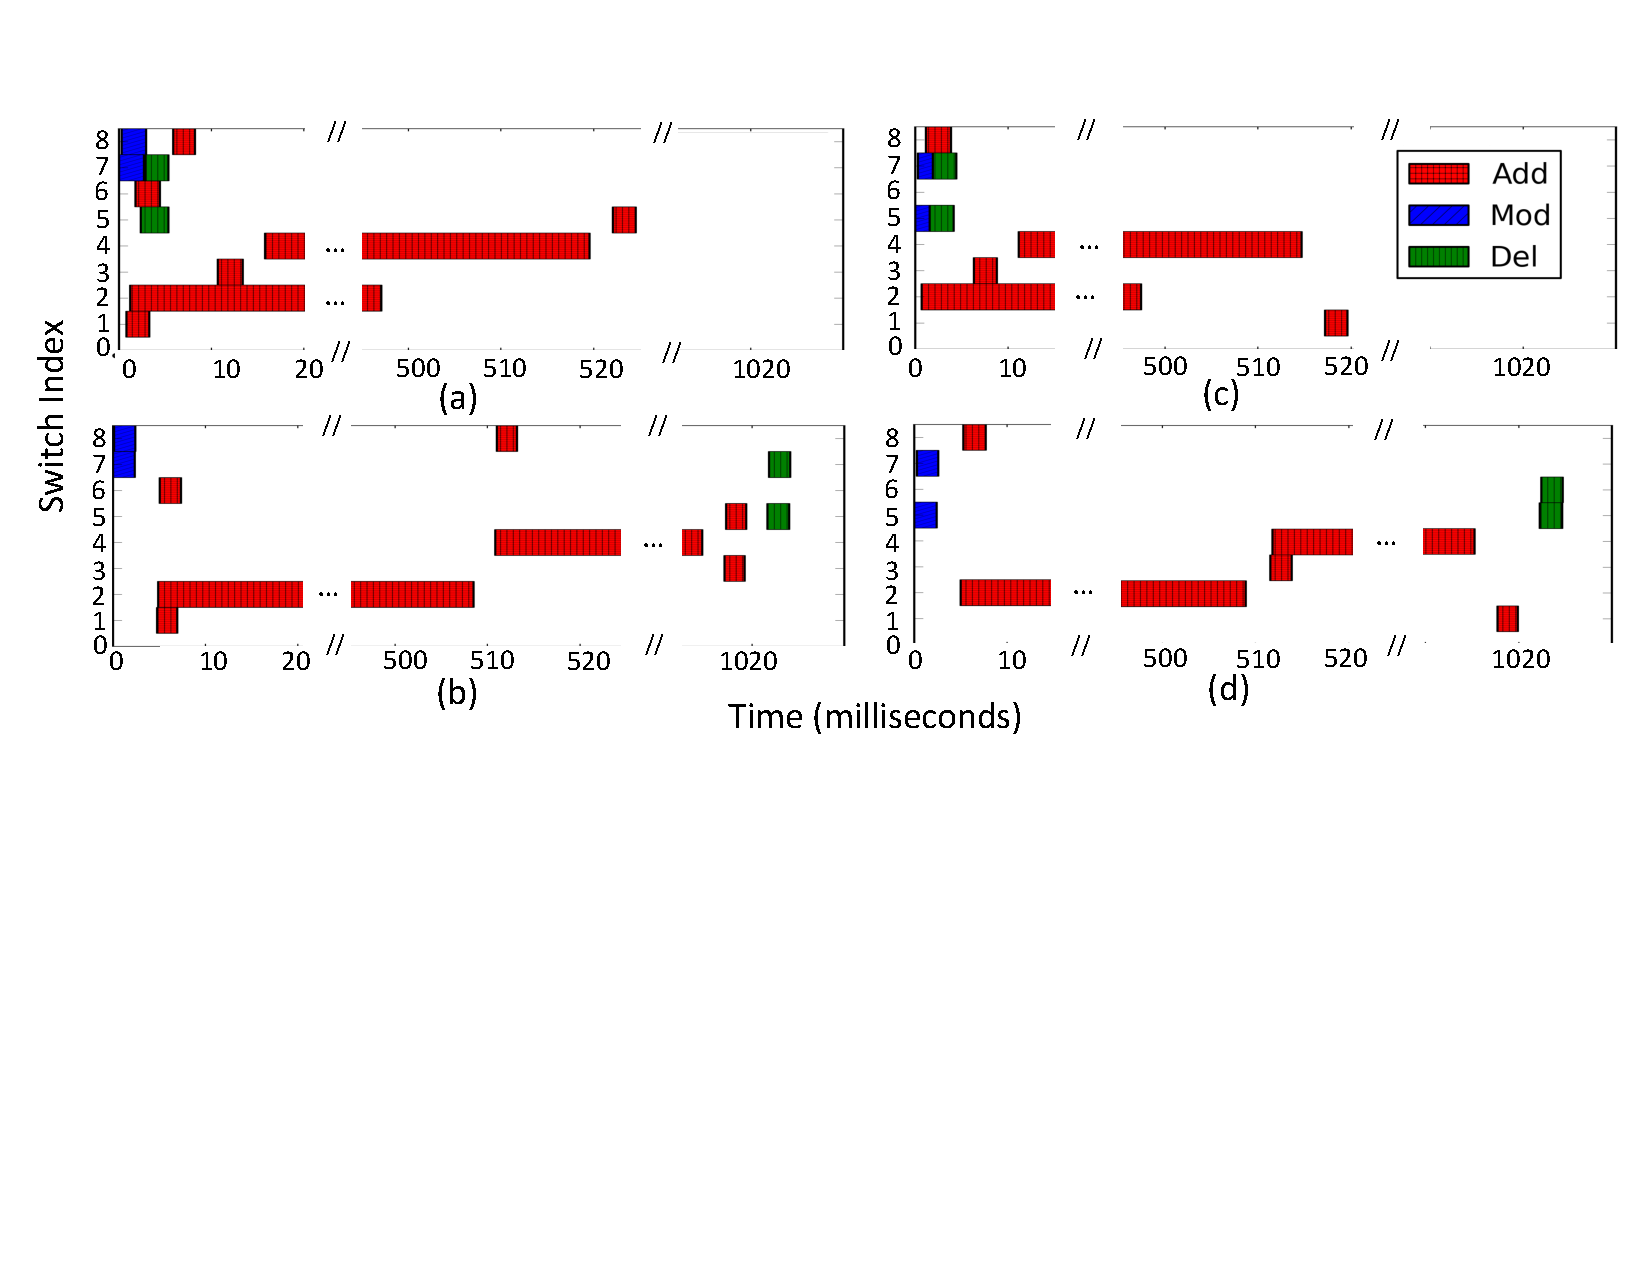
\includegraphics[width=0.8\textwidth]{figs/bandwidth}
        \end{minipage}
\end{figure*}

\section{Implementation}
\label{sec:impl}
We implemented a prototype of \name with 8000+ lines of C++ code. \name is
a shim layer between an SDN controller and network devices, 
intercepting and scheduling network updates issued by the
controller in real time. 
%It verifies the updates and synthesizes a correct
%ordering of updates to preserve consistency during network transition. 

\name maintains several types of state, including network-wide data plane
rules, the uncertainty state of each rule, the set of buffered updates, and bandwidth
information (e.g., for congestion-free invariants). It stores data plane rules
within a multi-layer trie in which each layer's sub-trie represents a packet header field.
We designed a customized trie data structure for handling different types of rule wildcards,
e.g., full wildcard, subnet wildcard, or bitmask wildcard~\cite{openflow-spec},
%differently,
%--- rules agnostic to matching on certain bits or fields, 
and a fast one-pass traversal algorithm to accelerate verification.
\wxzcr{
To handle wildcarding for bitmasks, each node in the trie has 
three child branches, one for each of \{0, 1, don't care\}. 
For subnetting, the wildcard branch has no children, but points 
directly to a next layer sub-trie or a rule set.
Thus, unlike other types of trie, 
the depth of subnet wildcard tries is not fixed as the number of bits in this field, 
but instead equals to the longest prefix among all the rules it stores.
Accordingly, traversal cost is reduced compared with general tries.
For full wildcard fields, values can only be non-wildcarded or full wildcarded.
The specialized trie structure for this type of field is a plain binary tree plus a wildcard table.

When a new update arrives, we need to determine the set of affected ECs,
as well as the rules affecting each EC.
VeriFlow~\cite{VeriFlow} performs a similar task via a two-pass algorithm,
first traversing the trie to compute a set of ECs, and then for each of the
discovered ECs, traversing the trie again to extract related rules.  In \name,
using callback functions and depth first searching, 
%we implemented in place checking, and 
the modeling work is finished with only one
traversal. This algorithm eliminates both the unnecessary extra pass over the
trie and the need to allocate memory for intermediate results.}
%we optimize this process by maintaining some additional accounting information,
%which lets us accomplish our similar objective in a single pass.  
%Our algorithm starts from the top layer subtrie, and combinations
%of its branches that match the first field of the update to be checked are
%selected. The traversal continues on the matched combinations, and would be
%further confined by the following fields of the update.  A matched combination
%of branches in the last level is an EC, and it already points to the rule set
%for that EC.  
%In
%addition, this approach results in a smaller number of ECs---each wildcard
%branch itself forms a matched combination.

In addition to forwarding rules, 
the data structure and algorithm are also capable of handling packet transformation rules, 
such as Network Address Translation (NAT) rules, and rules with VLAN tagging, which are used by CU for versioning, and verified by \name when the CU plug-in is triggered (see \S\ref{sec:eval}).

%\wxznew{
%One special case is dealing with packet transformation rules. 
%When such a rule is encountered during graph traversal phase, a new pass over the trie
%for the transformed EC is triggered. 
%Note that the graph is constructed while traversing rules, so only rules encountered 
%before transformation are kept, and the remaining rule set is discarded.
%More importantly, in this case, multiple trie traversals are possible, but only when 
%necessary, i.e., when a transformation rule is possibly forwarding packets for the original EC.
%} 

To keep track of the uncertainty states of rules, we design a compact state machine, which enables \name to detect rules that cause potential race conditions. If desired, our implementation can be configured to insert barrier messages to serialize those rule updates.

To bound the amount of time that the controller is uncertain about network states, 
we implemented two alternate types of the confirmation mechanisms: (1) an application-level acknowledgment by
modifying the user-space switch program in Mininet, and (2) leveraging the
barrier and barrier reply messages for our physical SDN testbed experiments.

\wxzcr{
%The way that \name stores and retrieves data plane rules is motivated by VeriFlow~\cite{VeriFlow}. 
%The essential idea is to build a multiple-layer trie, with each layer sub-trie 
%representing a packet header field. 
%Each level of a sub-trie corresponds to a bit of that \cut{packet header} field.
%%and can be one of three possible values: $0$, $1$, or wildcard.
%An upper layer sub-trie contains pointers on leaves to sub-tries in the next layer. 
%Dataplane rules are stored at the leaves of bottom sub-tries.
%A path from the root to a leaf of a bottom sub-trie determines a packet set, and one or more such sets can be merged together to form an \emph{equivalence class} (EC) of packets, \matt{i.e.,}
%%More formally, an \emph{equivalence class} (EC) is 
%a set of packets experiencing the same behaviors \wxznew{throughout the network}\cut{at any network device}.
%Upon arrival of an update, its effect on the network state is checked, by limiting searching to ECs whose behavior may be affected by this update, and building a graph model for each affected EC.
%However, given the need to store multiple different representations of the network state, the storage and processing overhead of \name could be larger than just maintaining a single snapshot, \matt{as done in} VeriFlow.
%\wxznew{
%Moreover, there are rules that perform packet transformation,
%such as Network Address Translation, i.e., these rules transform packets from one
%EC to another EC. To accurately model network behaviors, we need to able to handle such rules,
%which are left out in our motivating work, Veriflow.
%To meet this end,
%}
%we design a scalable data structure and an efficient algorithm to operate on it.

%\paragraphb{Customized Trie Data Structure}
%To scale the data structure,
%besides the general type of trie, we design two types of customized trie structure. 
%\matt{
%One complication is dealing with {\em wildcards} -- rules agnostic to matching on certain bits
%or fields. Wildcards complicate the traversal process, as multiple branches may need to be traversed, and the manner
%in which they are traversed can depend on the semantics of the rule (e.g., standard wildcards vs. longest-prefix match).
%To address this, we construct an algorithm that handles general bitmasking, then extend it with optimizations
%to more efficiently handle two common-case wildcard patterns: full wildcards (the entire field is wildcarded) and subnet mask (all bits
%less than a certain significance are wildcarded).  }

%\paragraphb{One-pass Traversal Algorithm}

%These efforts together with a highly optimized implementation 
%allow \name to run almost 100X faster compared to VeriFlow
%%despite having all the challenges we listed.
%with 15X less memory overhead% (540MB vs. 9GB).
%(\S\ref{sec:microbenchmark}). 
%One of our ongoing works is exploring the parallel implementation of the data structure.

%Similar to our prior work~\cite{VeriFlow}, 
\name exposes a set of APIs that can be used to write general queries in C++.
The APIs allow the network operator to get a list of affected equivalence 
classes given an arbitrary forwarding rule, the corresponding 
forwarding graphs, as well as traverse these graphs in a controlled manner 
and check properties of interest. For instance, an operator can ensure
packets from an insecure source encounter a firewall before accessing an internal server.
%To ensure this invariant, \name can be extended using the above APIs to incorporate 
%a custom query algorithm that reports an violation when the packet from that source bypasses the firewall.
}


\section{Evaluation}
\label{sec:eval}

%In this section, we present the performance evaluation of \name from three aspects. Can \name verify network invariants in real time (\S\ref{sec:microbenchmark})? Can \name achieve performance gain during network transitions  (\S\ref{sec:parallel})? Can  \name detect more types of network faults with the uncertainty-aware network model (\S\ref{sec:bug-coverage})? 

\subsection{Verification Time}
\label{sec:microbenchmark}

%We first conduct speed analysis of \name with comparison of an existing \emph{real-time} data-plane network verifier, VeriFlow~\cite{VeriFlow}. 
To gain a baseline understanding of \name's performance, we micro-benchmarked how long the verification engine takes to verify a single update.
%We simulated a network consisting of 172 routers following a Rocketfuel topology (AS 1755)~\cite{Rocketfuel}. 
We simulated BGP routing changes by replaying traces collected from the Route Views Project~\cite{RouteViews}, 
on a network consisting of 172 routers following a Rocketfuel topology (AS 1755)~\cite{Rocketfuel}.
%We created an OSPF (Open Shortest Path First) simulator to compute the IGP (Interior Gateway Protocol) path cost between every pair of routers in the network. A BGP RIB snapshot consisting of 5 million entries was used to initialize the routers' FIB (Forwarding Information Base) tables. We randomly mapped Route Views peers to border routers in our network, and then replayed RIB and update traces so that they originate according to this mapping. We replayed a BGP update trace containing 90,000 updates to trigger dynamic changes in the network. Upon receiving an update from the neighboring AS, each border router sends the update to all the other routers in the network. Using standard BGP polices, each router updates its RIB using the information present in the update, and updates its FIB based on BGP AS path length and IGP path cost. 
After initializing the network with 90,000 BGP updates, 2,559,251 updates were fed into \name and VeriFlow~\cite{VeriFlow} (as comparison).
We also varied the number of concurrent uncertain rules in \name from 100 to 10,000. All experiments were performed on a 12-core machine with Intel Core i7 CPU at 3.33 GHz, and 18 GB of RAM, running 64-bit Ubuntu Linux 12.04. The CDFs of the update verification time are shown in Figure~\ref{fig:microbench}.

\begin{figure}[!ht]
  \centering
  \vspace{-0.15in}
  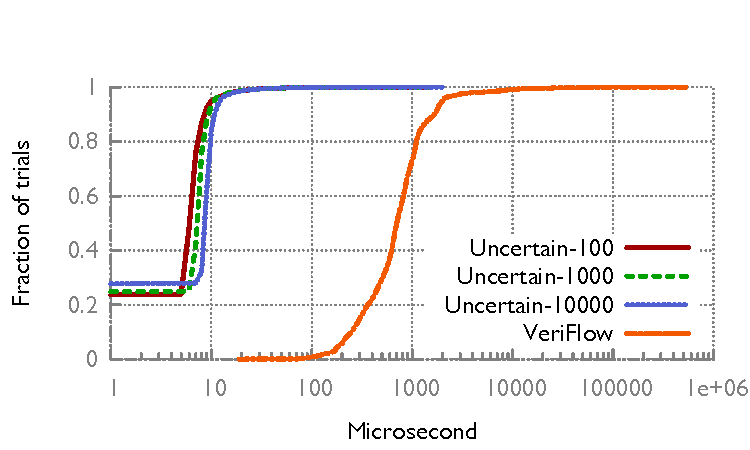
\includegraphics[width=\columnwidth,trim= 0 5mm 0 10mm]{figs/micro}
  \vspace{-0.2in}
  \caption{\em \small Microbenchmark results.}
  \vspace{-0.15in}
  \label{fig:microbench}
\end{figure}

%We observed that 
\name was able to verify 80\% of the updates within 10 $\mu$s, with a 9 $\mu$s mean. 
%In fact, approximately 25\% of the updates were verified within 1 $\mu$s. The reason is that only the minimum change to \name's network model is required for each update, i.e., only one operation in the trie, as indicated by Figure \ref{fig:statemachine}. 
%\wxzc{This sentence (the one refers to fig 8) was used to explain the sentence before it, which is comment off now. So this one needs to be rewritten.}
\name verifies updates almost two order of magnitude faster than VeriFlow because of 
data structure optimizations (\S\ref{sec:impl}). 
Approximately 25\% of the updates were processed within 1 $\mu$s, 
because \name accurately tracks the state of each rule over
time. When a new update matches the pattern of some existing rule, it's likely
only a minimum change to \name's network model is required (e.g., only one
operation in the trie, with no unnecessary verification triggered).
We observed long tails in all curves, but the verification time of \name is bounded by 2.16 ms, almost three orders of magnitude faster than VeriFlow's worst case. 
%which is tolerable for most wide-area network applications. 
%\wxzc{do we need to emphasize ``wide-area" here?}
The results also show strong scalability. As the number of concurrent uncertainty rules grows, the verification time increases slightly (on average, 6.6 $\mu$s, 7.3 $\mu$s, and  8.2 $\mu$s for the 100-, 1000-, and 10000-uncertain-rule cases, respectively). Moreover, \name offers a significant memory overhead reduction relative to VeriFlow: 540 MB vs 9 GB.


%\subsection{Performance Analysis during Network Changes}
\subsection{Performance Analysis}
\label{sec:parallel}

\subsubsection{Emulation-based Evaluation}
%\paragraphb{Emulation-based Evaluation}

\paragraphe{Segment-independent Policies:}
We used Mininet to emulate a fat-tree network with a shortest path routing application and a load-balancing application in a NOX controller. The network consists of five core switches
%\cut{fully connected with} 
and ten edge switches, and each edge switch connects to five hosts. %To initialize the flow table for each switch, each host first picked up a random destination host to perform a file transfer. 
Once the rules were stable in the switches, we changed the network (e.g., add links, or migrate hosts) to trigger the controller to update the data plane with a set of new updates. %We measured the delay that the new rules took to be applied to the network. 
For each set of experiments, we tested six update mechanisms: (1) the controller immediately issues updates to the network (``Optimal" in terms of update speed); (2) \name with the basic connectivity invariant (loop and black-hole freedom) verification enabled (\name); (3) \name with an additional invariant that packets must traverse a specific middle hop before reaching the destination (\name-waypoint); (4) Consistent Updates (CU)~\cite{Reitblatt2012}; (5) incremental Consistent Updates (Incremental CU)~\cite{incremental-cu}; and (6) Dionysus \cite{jin2014dynamic} with its WCMP forwarding dependency graph generator.
\wxznew{We configure our applications as the same type as in Dionysus, with
forwarding rules matching exactly one flow, i.e., no overlapping forwarding
graphs. Thus, loop and black-hole freedom are segment-independent as proved in
\S\ref{sec:seg-independence}. Because of the fat-tree structure, there is no
crossing between path segments (as in Fig~\ref{fig:circular}(a)), 
so the waypoint policy is also segment independent.}
\wxzcr{A mix of old and new configurations, e.g., 
$oldAB + newBC$ in Figure~\ref{fig:circular}(a), 
is allowed by \name, but forbidden when using CU.}

%The CU we used was modified from an implementation developed at Stanford University \cite{standford_cu_imp}. Each experiment was repeated 10 times and we plotted the experimental results in the form of CDF. 

%Here we define {\em controller-switch delay} as the delay between controller issuing an update and the corresponding switch finishing the application of the update. The controller-switch delay is the sum of networking delay (typically on the order of hundreds of microseconds in data center networks), and processing delay (the time a switch takes to apply an update, e.g, installing a flow entry). Flow entry installation speed of commercial SDN switches like Pica8 is around 200 flows per second. 
We first set the delay between the controller issuing an update and the corresponding switch \wxznew{finishing the application of} the update (i.e, the controller-switch delay) to a normal distribution with 4 ms mean and 3 ms jitter, to mimic a dynamic data center network environment. The settings are in line with that of other data center SDN experiments~\cite{curtis2011devoflow, Sherwood10}. We initialized the test with one core switch enabled and added the other four core switches after 10 seconds. The traffic eventually is evenly distributed across all links because of the load balancer application. We measured the completion time of updating each communication path, %, i.e. the completion time of the last update on the path, 
repeated each experiment 10 times.  Figure~\ref{fig:emulation}(a) shows the CDFs for all six scenarios.

The performance of both ``$CCG$" and ``\name-waypoint" is close to optimal, and much faster \kevin{(47 ms reduction on average)} than CU. %To avoid the rare situations of infeasible update orderings with pure \name (though we did not encounter any in this set of experiments), we integrated the \name with CU to ensure the same consistency level (e.g., absence of black holes and loops). 
%``\name+CU" is 15 ms slower than \name alone in average because of the additional cost of packet transformation, versioning, and rule classification, but it is still 20 ms faster in average than CU. 
%It is because CU holds the network invariants by ensuring that all packets can only be handled by either the old rules or the new rules via a two-phase update mechanism. 
In CU, the controller is required to wait for the maximum controller-switch delay to guarantee that all packets can only be handled by either the old or the new rules. 
%across all the switches, before proceeding to phase two to complete the update. 
\name relaxes the constraints by allowing a packet being handled by a mixture of old and new rules along the paths, as long as the impact of the new rules passed verification. By doing so, \name can apply any verified updates without explicitly waiting for irrelevant updates. 
%In addition, \name can aggregate more updates to individual network devices. CU or incremental-CU, on the other hand, have to distinguish {\em edge rules} and {\em internal rules} and apply them in separate phases. \wxzc{not sure it's necessary to mention the benefit of aggregation?} 
%The memory usages for all five scenarios are presented in \fixme{Figure X}. 
CU requires temporary doubling of the FIB space for each update, %Many SDN switches use TCAM memory, which is both expensive and power-consuming. It is because in CU, packets handled by each configuration are tagged with different version numbers to avoid encountering a mix of configurations. 
because it does not delete old rules until all in-flight packets processed by the old configuration have drained out of the network. To address this, incremental-CU was proposed to trade time against flow table space. By breaking a batch of updates into $k$ subgroups ($k=3$ in our tests), incremental-CU reduced the extra memory usage to roughly one $k$th at the cost of multiplying the update time $k$ times. %but took much longer to apply all updates ($k$ times of the delay using CU). 
\wxznew{In contrast, when dealing with segment-independent policies, as in this set of experiments,} \name never needs to trigger any heavyweight fallback plug-in, and thus requires no additional memory, which is particularly useful as switch TCAM memory can be expensive and power-hungry.

%Also, \name reduces the expensive packet modifications that are required by the CU design to enforce versioning. We also observed in Figure~\ref{fig:emulation}(a) that the verification process only adds a little overhead to the update completion time as compared with the optimal case. 

%The second set of experiments evaluated the system update delay with dynamic host settings. We used all five core switches and ten edges switches throughout the experiments. Initially, each host sent traffic to another randomly selected host. After 10 seconds, we randomly re-distributed 40\% of the connections between hosts and edge switches, and then started the file transfer again. The results are in Figure~\ref{fig:emulation}(b). We observed that the gap between \name and the optimal case is larger (around 30 ms) than the results in the first set of experiments. It is because host position changes resulted in almost a complete change of the relevant paths, and thus complicates the inter-dependency among the new rules. But still \name outperformed CU by 20 ms per update on average. 

\begin{figure}[!th]
  \centering
  \vspace{-0.1in}
  \subfigure[Data center network setting]{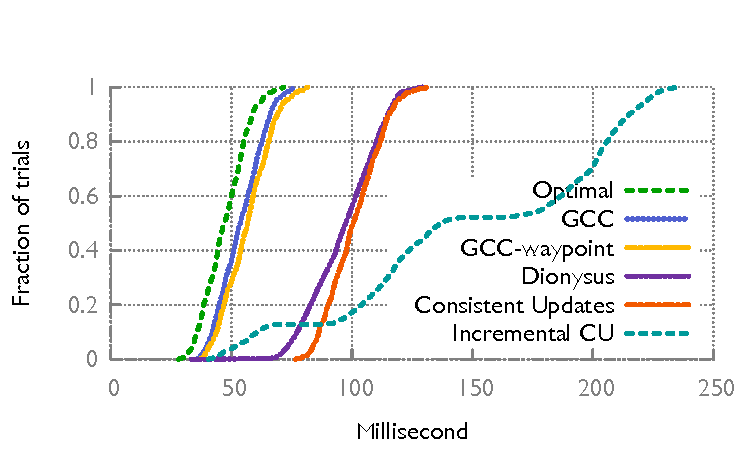
\includegraphics[scale=0.6,trim=0mm 0mm 0mm 10mm]{figs/emulation_4ms}}%
  \vspace{-0.1in}
  %\subfigure[Data Center Network, Transition with Host Migration]{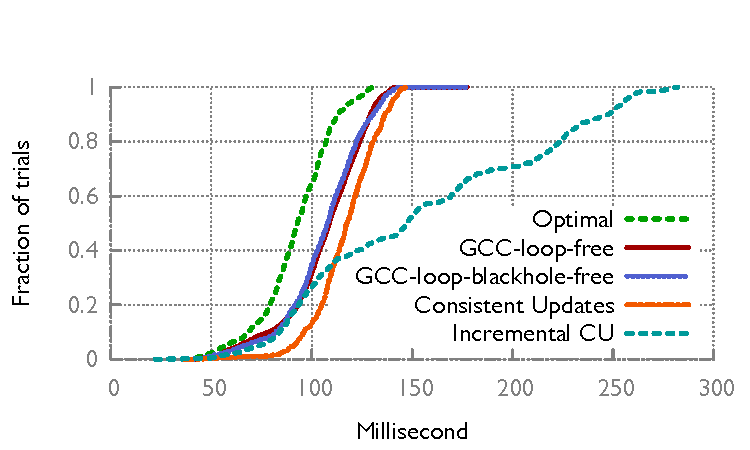
\includegraphics[scale=0.6,trim=0mm 0mm 0mm 1mm]{figs/emulation_dynamic_1ms}}
  \subfigure[Wide-area network setting]{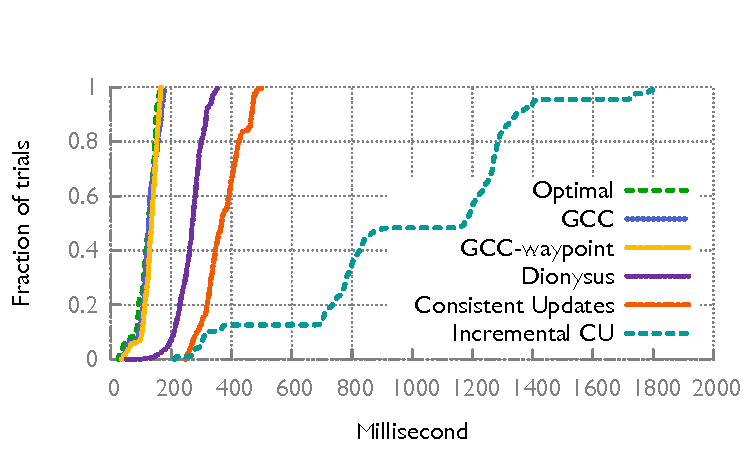
\includegraphics[scale=0.6,trim=0mm 0mm 0mm 1mm]{figs/emulation_100ms}}
  %\subfigure[Wide-area Network, Transition with Host Migration]{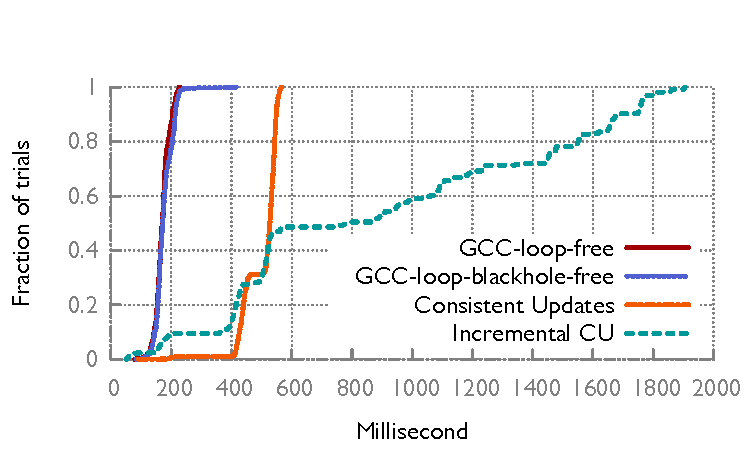
\includegraphics[scale=0.6,trim=0mm 0mm 0mm 1mm]{figs/emulation_dynamic_25ms}}
  %\vspace{10pt}
  \vspace{-0.1in}
  \caption{\em \small Emulation results: update completion time comparison.}
  \vspace{-0.3in}
  \label{fig:emulation}
\end{figure}

To understand how \name performs in wide-area networks, 
where SDNs have also been used~\cite{jain2013b4, Hong13}, 
we set the controller-switch delay to 100 ms (normal distribution, 
with 25ms jitter), and repeated the same tests (Figure \ref{fig:emulation}(b)). 
\name saved over 200 ms update completion time compared to CU,  mainly due to the longer controller-switch delay, for which CU and incremental-CU have to wait between the two phases of updates. %Besides the network changes with link addition, we also experiment the systems with dynamic host migration, and observed the similar performance gain of \name as compared with CU and ICU. 

\wxznew{
As for Dionysus, 
we observed in Figure~\ref{fig:emulation}
that it speeds up updates compared to CU in both local and wide-area
settings, as it reacts to network dynamics rather than pre-determineing a
schedule. But because its default algorithm for WCMP forwarding produces
basically the same number of updates as CU, 
\name (either \name or \name-waypoint)
outperforms it in both time and memory cost.
We further compared \name-waypoint with Dionysus in other dynamic situations, 
by varying controller-switch delay distribution.
Figure~\ref{fig:dn} shows the $50^{th}$, $90^{th}$ and $99^{th}$ percentile 
update completion time, under various controller-switch delays
(normal distributed with different (mean, jitter) pairs, $(a, b)$) for 
four update mechanisms: optimal, \name, Dionysus, and CU. 
In most cases, both \name and Dionysus 
outperform CU, with one exception (4ms delay, zero jitter).
Here, Dionysus does not outperform CU because
it adjusts its schedule according to network dynamics, 
which was almost absent in this scenario.
The cost of generating dependency graphs in this scenario
is relatively large compared to the small network delay.
When the mean delay was larger (100ms), even with no jitter,
Dionysus managed to speed the transition by updating each forwarding path independently.}
On the other hand, \name's performance is closer to the Optimal case than Dionysus. For example, in the $(4, 0)$ case,  \name is 37\%, 38\%, and 52\% faster than Dionysus in the $50^{th}$, $90^{th}$ and $99^{th}$ percentile, respectively; in the $(100, 25)$ case,  \name is 50\%, 50\%, and 53\% faster than Dionysus in the $50^{th}$, $90^{th}$ and $99^{th}$ percentile, respectively. Also, we observe that Dionysus's performance is highly dependent on the variance of the controller-switch delay (the larger the jitter is, the faster the update speed) because of the dynamic scheduling, but \name's performance is insensitive to the jitter.

\begin{figure}[!ht]
  \centering
  \vspace{-0.1in}
  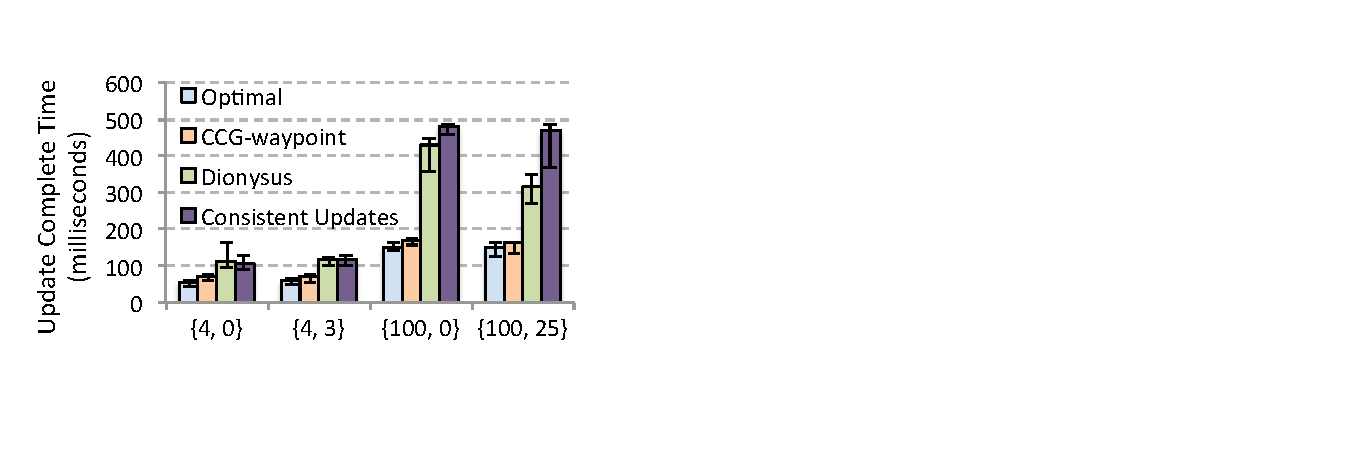
\includegraphics[width=0.8\columnwidth]{figs/distribution_narrow.pdf}
  \vspace{-0.1in}
  \caption{\em Update completion time with [$50^{th}$, $90^{th}$, $99^{th}$ percentile]; x-axis label \{a, b\}: a is the mean controller-switch delay, b is the jitter following a normal distribution.}
  \vspace{-0.2in}
  \label{fig:dn}
\end{figure}

\paragraphe{Non-segment-independent Policies:}
\kevin{
We then explored scenarios in which \name's lightweight heuristic cannot always synthesize a correct update ordering and needs to fall back to the more heavyweight algorithm to guarantee consistency. The traces we used were collected from a relatively large enterprise network that consists of over 200 layer-3 devices.
%\cut{Each device has around 13,000 to 15,000 rules in average.}
\wxznew{During a one-day period (from 16:00 7/22/2014 to 16:00 7/23/2014), we took one snapshot of the network per hour, and used Mininet to emulate 24 
transitions, each between two successive snapshots.}
%\cut{The data covers the duration of one day (from 16:00 7/22/2014 to 16:00
%7/23/2014), and was divided into 24 one-hour windows. For each window, we
%took a new snapshot of the network states, and performed a transition from
%the previous snapshot to the current one. }
We processed the network updates
with three mechanisms: immediate application of updates, \name, and CU.
\wxzcr{Updates were issued such that new rules were added first, then old rules deleted.
Thus, all three mechanisms experience the trend that the number of stored rules increases
then decreases.}.
The controller-switch delay was set to 4 ms. We selected 10 strongly
connected devices in the network, and plotted the number of rules 
in the network over time during four transition windows, as shown in
Figure \ref{fig:cise}. As the collected rules overlapped with longest prefix match,
the resulting forwarding graphs might share links, so unlike previous experiments,
segment-independency was not guaranteed.

%We observed 
The update completion time (\wxznew{indicated by the width of
the span of each curve}) using \name was much shorter
%(around x\% shorter on average with the standard deviation y\%) 
than CU, and the memory
needed to store the rules was much smaller.
%(around x\% smaller on average, with the standard deviation y\%). 
In fact, the speed and memory requirements of \name 
were close to those of the immediate update case, because
\name rarely needs to fall back to CU. In 22 out of 24
windows, there was a relatively small number of network updates (around 100+),
much as in the [22:00, 23:00) window shown in Figure \ref{fig:cise},
%\wxzc{This window is an example of one of the windows}
in which \name
passed through most of the updates with very few fallbacks. During the period 23:00
to 1:00, there was a burst of network dynamics (likely to have been 
caused by network maintenance), in which 8000+ network
updates occurred. Even for such a large number of updates, the
number of updates forced to a fallback to CU, was still quite small (10+).
\wxzcr{Since \name only schedules updates in a heuristic way,
the waiting time of a buffered update could be suboptimal, as in this hour's case,
where the final completion time of \name was closer to CU.}
%\cut{In addition, even for the fall back scenarios, the
%rules that triggers the fallbacks are actually a subset of the entire rules
%required by CU, which essentially} 
%Thus we can see, \name significantly reduces the
%memory requirement and increases the processing speed. On the other hand,
\name achieves performance comparable to the immediate update mechanism, but without
any of its short-term network faults (24 errors in the 0:00 to 2:00 period).

%With performance typically comparable to the immediate update mechanism,
%(the ideal case in terms of speed and memory), 
%\name did not suffer from any short-term
%network fault as the immediate update did
%\cut{due to inconsistence updates} 
%(e.g., 24 errors in the 0:00 to 2:00 period). 
%This demonstrates \name's ability to achieve nearly the
%``best of both worlds": the efficiency of passing through updates in
%most cases, with the consistency guarantees of more heavyweight solutions.  
}

%handle packet transformation
%during fall back, also handle packet transformation
%this time, prefix matching -> one rule affect multiple forward graphs. the orders from graph maybe conflict
%in fat tree topo + exact matching

\begin{figure*}[!ht]
  \vspace{-0.1in}
  \centering
  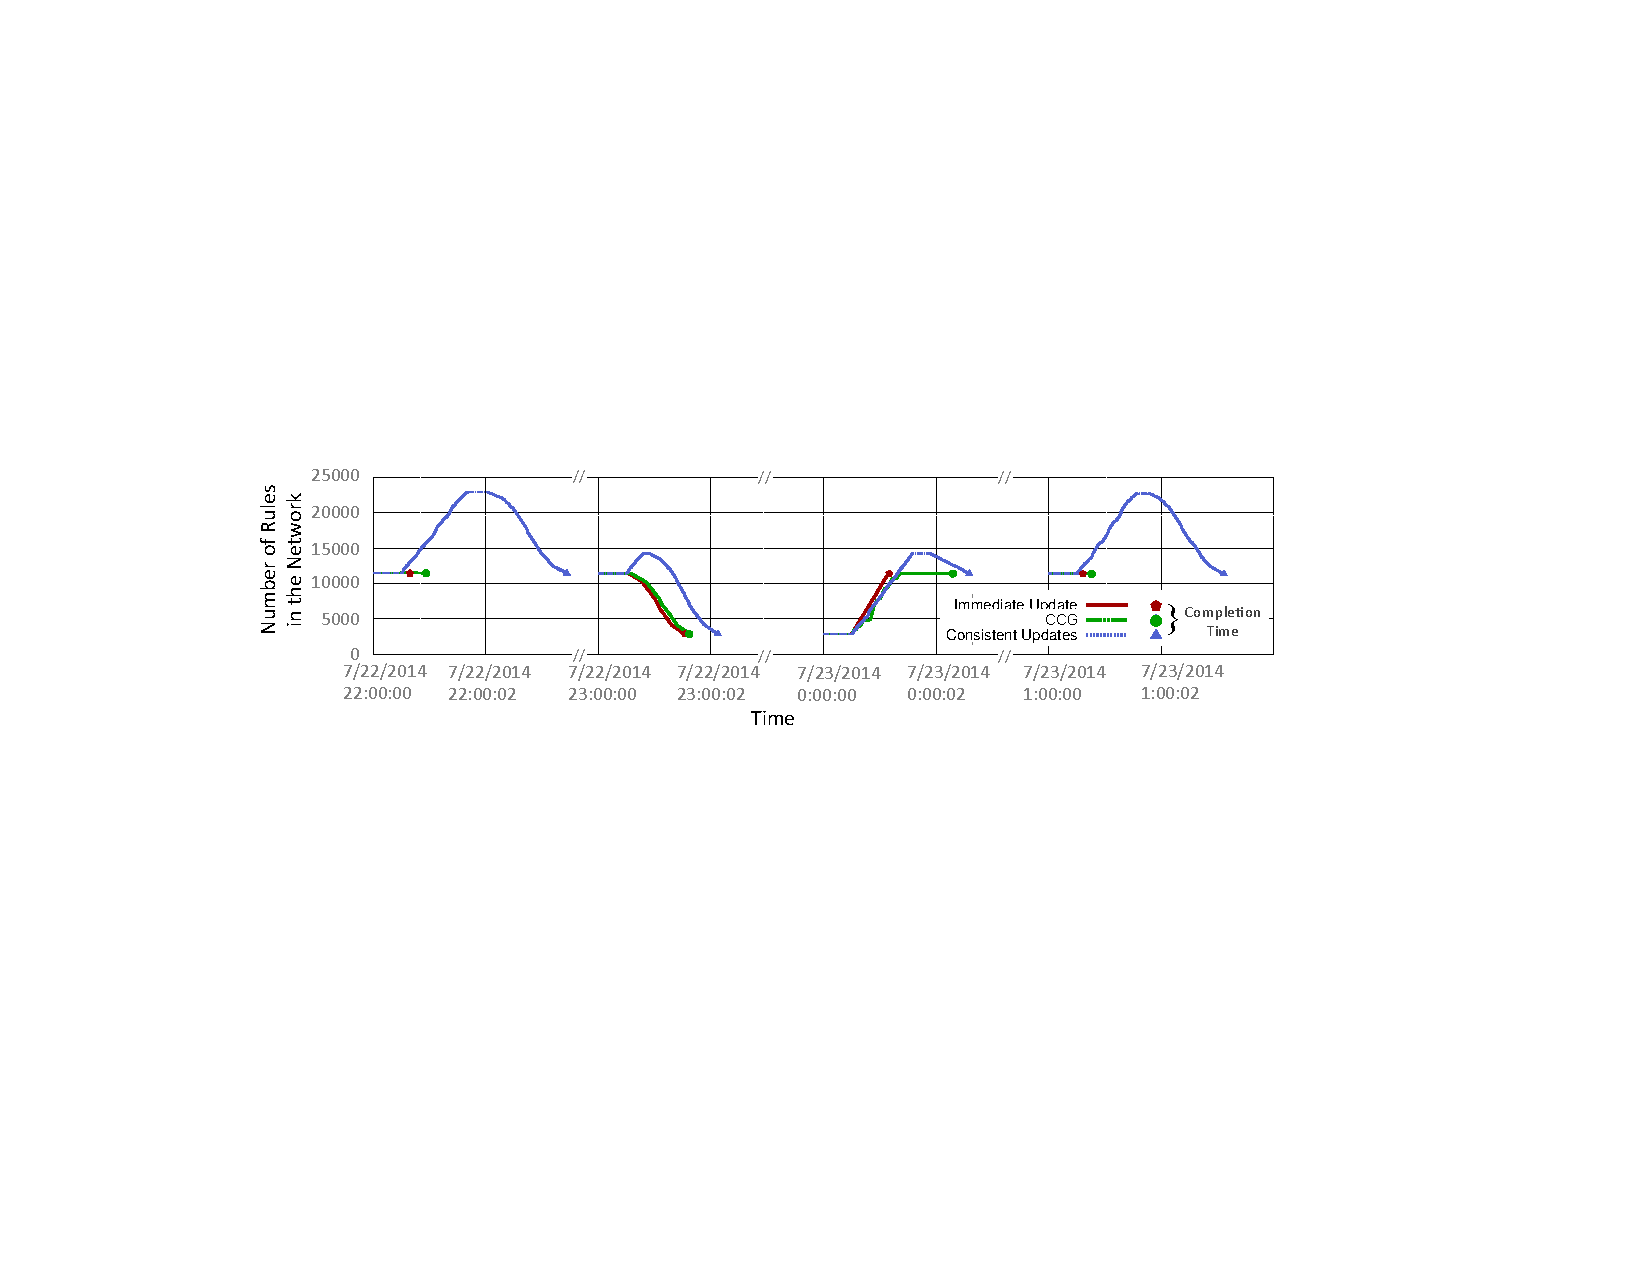
\includegraphics[width=\textwidth]{figs/count.pdf}
  \vspace{-0.3in}
  \caption{\em Network-trace-driven emulations: (1) immediate application of updates; (2) \name (with CU as fallback); and (3) CU.}
  \vspace{-0.2in}
  \label{fig:cise}
\end{figure*}


\subsubsection{Physical-testbed-based Evaluation}
%To test real world distributed timing effects, 
%\paragraphe{Physical-testbed-based Evaluation:}
We also evaluated \name on a physical SDN testbed~\cite{ocean}
consisting of 176 server ports and 676 switch ports, using Pica8 Pronto 3290 switches via TAM Networks, NIAGARA 32066 NICs from Interface Masters, and servers from Dell.
We compared the performance of \name and CU by monitoring the traffic
throughput during network transitions. We first created a network
with two sender-receiver pairs transmitting TCP traffic on gigabit links, 
shown in Figure \ref{fig:s_topo}. Initially, a single link was shared by the
pairs, and two flows competed for bandwidth.  After 90 seconds, another path
was added %\cut{for one of the pairs}
(the upper portion with dashed lines in
Figure \ref{fig:s_topo}). Eventually, one flow was migrated to
the new path and each link was saturated. 
% We are interested to explore the system behaviors during the network changes. 
We repeated the experiment 10 times, and recorded the average throughput in a 100-ms window during the network changes. We observed repeatable results.  Figure~\ref{fig:testbed}(a) shows the aggregated
throughput over time for one trial.

\name took 0.3 seconds less to finish the transition than CU because: (1) unlike CU, \name does not require packet modification to support versioning, which takes on the order of microseconds for gigabit links, while packet forwarding is on the order of nanoseconds; (2) CU requires more rule updates and storage than \name, and the speed of rule installation is around 200 flows per second; and (3) Pica8 OpenFlow switches (with firmware 1.6) cannot simultaneously process rule installations and packets.\footnote{All the performance specifications reported in this paper have been confirmed with the Pica8 technical team.} %We also noticed that, besides delayed network transition, the amount of the extra work required by CU also resulted in some temporary throughput drops (as shown in Figure \ref{fig:testbed}(a)). 
%because of the long rule processing and buffering time. 
%However, such drops did not occur in \name throughout all of our experiments.

\begin{figure}[!ht]
  \centering
  \vspace{-0.1in}
  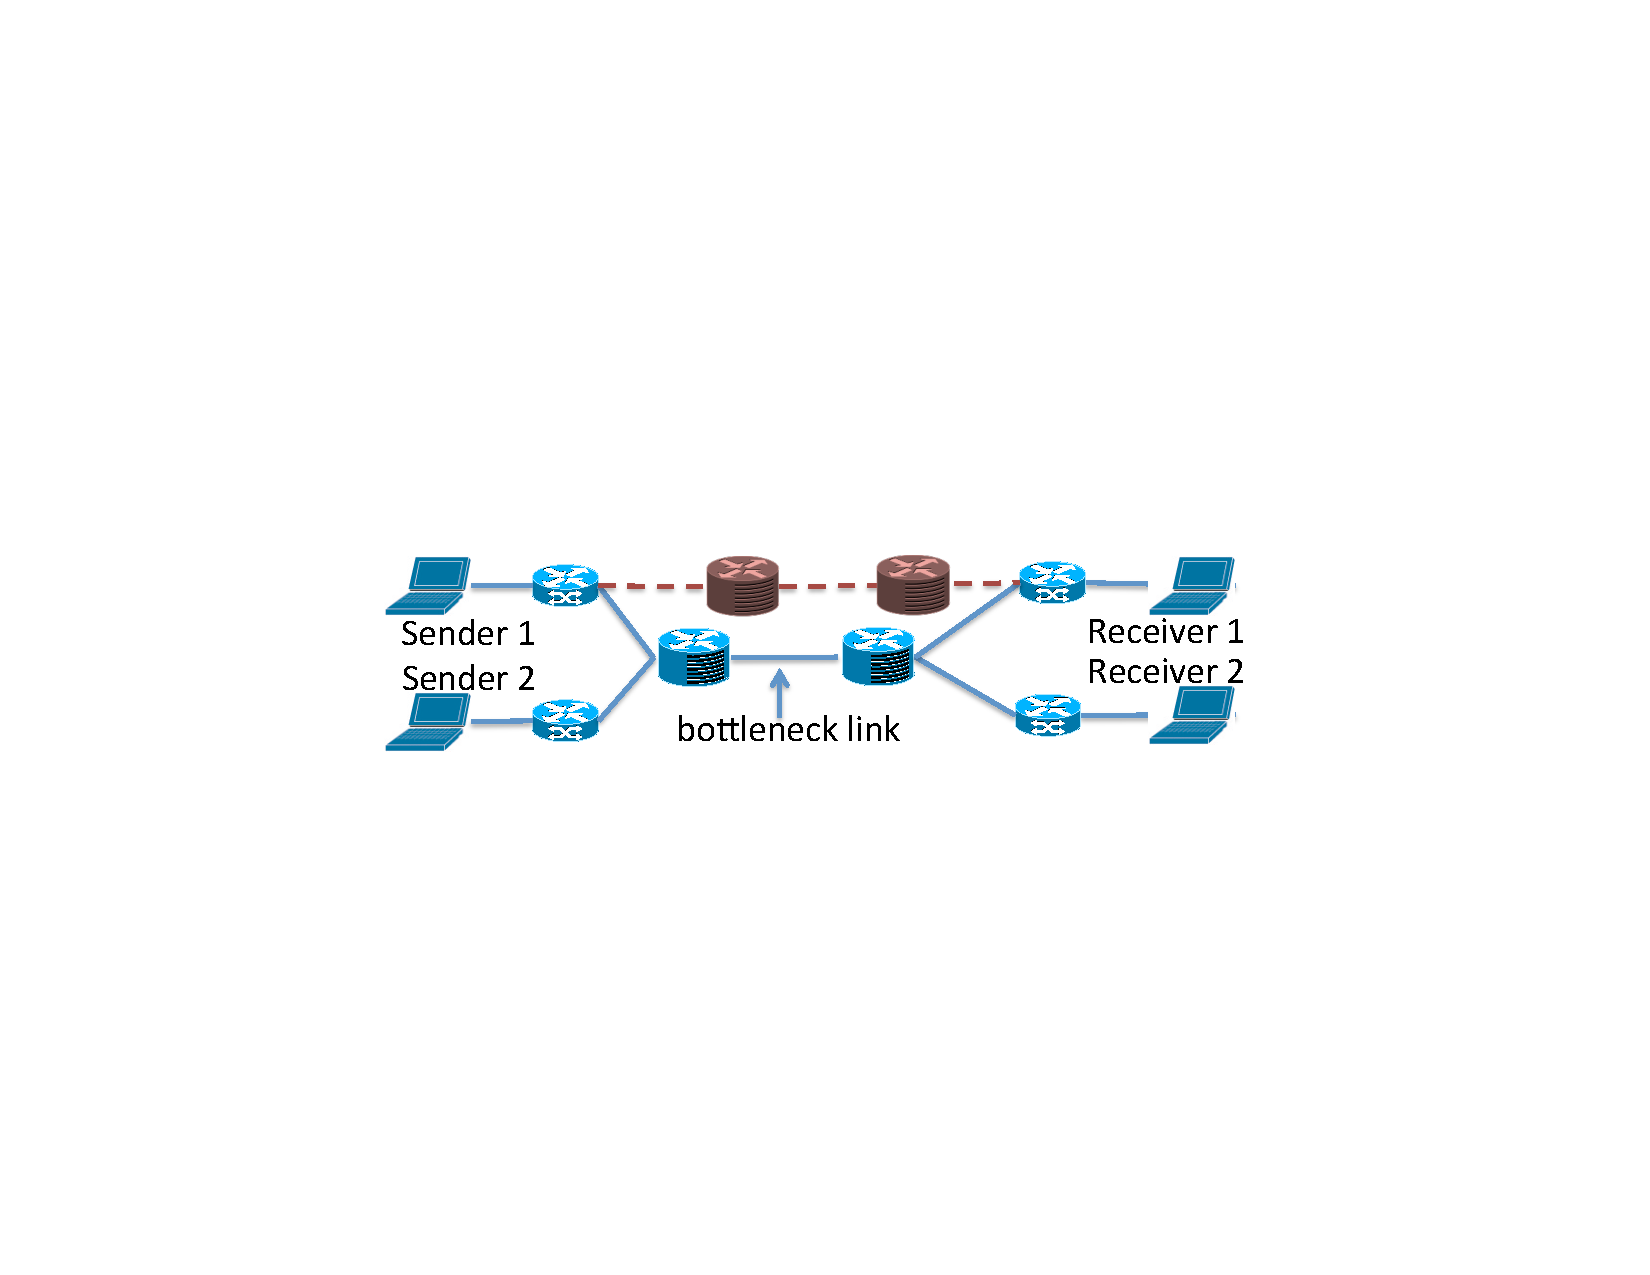
\includegraphics[width=0.7\columnwidth]{figs/dumbell_topo}
  \vspace{-0.1in}
  \caption{\em eight-switch topology.}
  \vspace{-0.15in}
  \label{fig:s_topo}
\end{figure}

\begin{figure}[!ht]
  \centering
  \vspace{-0.1in}
  \subfigure[A eight-switch topology.]{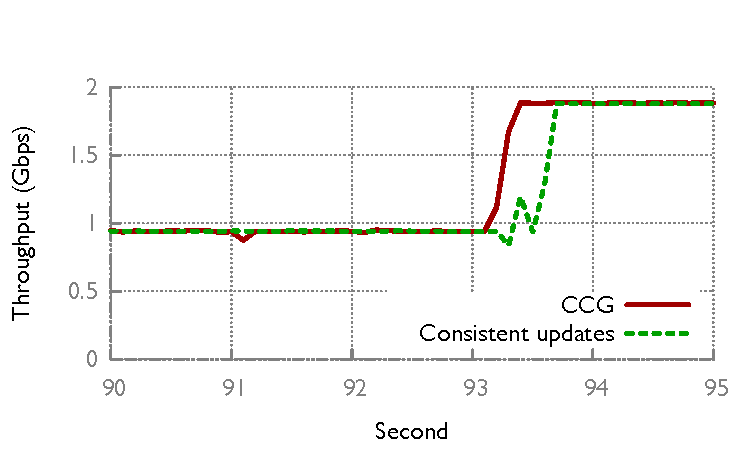
\includegraphics[width=0.8\columnwidth,trim=0mm 0mm 0mm 12mm]{figs/testbed_subspace_small}}%
  \vspace{-0.1in}
  %\subfigure[Throughput Changes during Network Transitions on a Small-scale Network with 6 Switches]{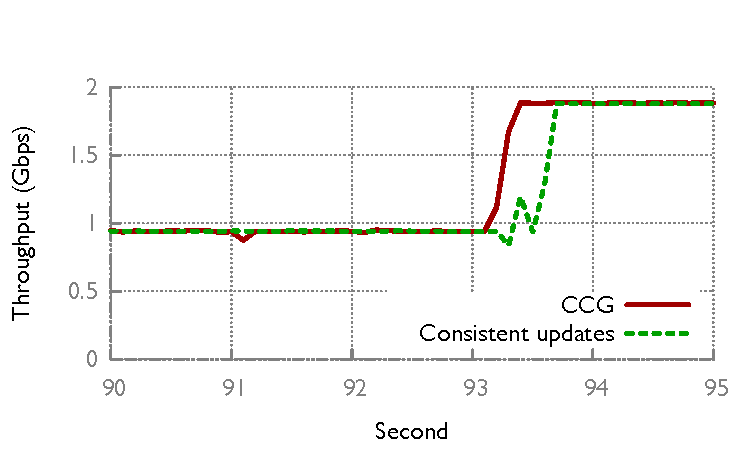
\includegraphics[width=\columnwidth,trim=0mm 0mm 0mm 12mm]{figs/testbed_subspace_small}}
  \subfigure[A 78-switch network.]{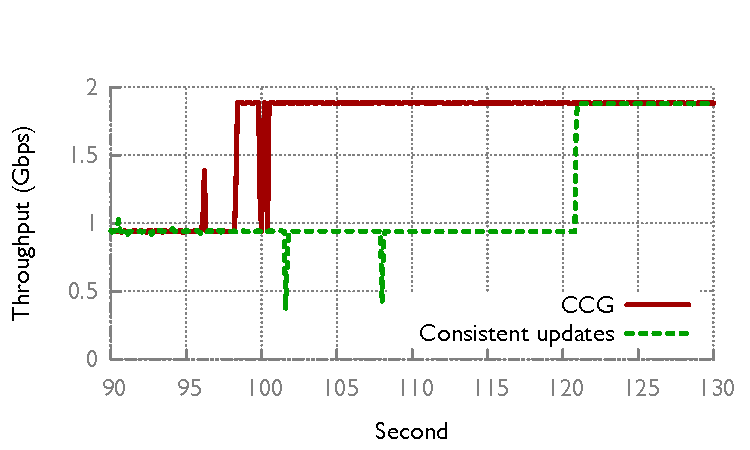
\includegraphics[width=0.8\columnwidth,trim=0mm 0mm 0mm 2mm]{figs/testbed_full}}
  \vspace{-0.1in}
  \caption{\em \small Physical testbed results: comparison of throughput changes during network transitions for \name and CU.}
  \vspace{-0.3in}
  \label{fig:testbed}
\end{figure}

%\if 0
%We created a biggest fat tree topology with X core switches and Y edge switches by slicing the 13 physical SDN switches. The virtual topology to physical topology mapping algorithm was developed using the GUROBI optimization package \cite{gurobi}. We are using same NOX controller applications as we used for the emulation experiments. Initially, we set the flow tables of the switches to enable only N core switches, and all hosts sent traffic to every other host for 10 seconds. We then alter the switch flow tables to bring in all the remaining core switches, and more flows would be migrated to the new core switches for load balancing. We measure the throughput and the flow drop rate for the CU, incremental CU, and \name for comparison. The results are shown in Figure \ref{fig:testbed}. [to change]
%\fi
\wxzcr{To test \name in a larger setting, 
%we then created a topology utilizing all 13 physical SDN switches. 
we then utilized all 13 physical switches. 
Each physical switch was devided into 6 ``virtual" switches by creating 6 bridges.
Due to the fact that the switches are physically randomly connected,
this division results in a ``pseudo-random" network consisting of 78 switches, each with 8 ports.} 
%Eight ports were attached to each virtual switch and the port assignment was computed with our mapping algorithm, which was developed using the GUROBI optimization package \cite{gurobi}. The mapping algorithm ensures that each attached virtual host had at least one path to every other host, subject to the physical cabling. 
Initially, the topology consisted of 60 switches, %and each switch was connected to two hosts. 
and we randomly selected 10 sender-receiver pairs to transmit TCP traffic. %, and each sender and the corresponding receiver were attached to different virtual switches. 
After 90 seconds, we enabled the remaining 18 switches in the network. 
The topology change triggered installations of new rules to balance load. % under the command of the NOX controller. 
We repeated the experiments 10 times, 
%and measured throughput of each flow. We 
and selected two flows from one trial that experienced throughput changes
%, and show the changes over time in a 100 ms window 
(Figure~\ref{fig:testbed}(b)). The trend of the two flows is consistent with the overall observed throughput change. %The selection criteria of the two flows are that they shared common links before the transition and used two disjoint paths after the transition, and there was no cross-traffic from other flows on their paths. %This way, comparison with the results in the first set of experiments under larger network state changes is straigtforward. The results are shown in Figure \ref{fig:testbed}(b). 

%We observed a similar trend as in the small topology setting; 
\name again outperformed CU in convergence time and average throughput during transitions. Compared to CU, \name spent 20 fewer seconds to complete the transition (a reduction of 2/3), because CU waits for confirmation of all updates in the first phase before proceeding to the second.
%, and the performance drops dramatically as the number of updates increases. 
In contrast, \name's algorithm significantly shortened the delay, especially for networks experiencing a large number of state changes. In \name, the throughput never dropped below 0.9 Gb/s, while CU experienced temporary yet significant drops during the transition, primarily due to the switches' lack of support for simultaneous application of updates and processing of packets. %\wxznew{We are still researching on the explanation, and one possible reason is switches' lack of support to parallelize operations.}


\if 0
\subsection{Network Fault Detection Coverage}
\label{sec:bug-coverage}

Failing to consider the temporal uncertainty of the network may result in transient or permanent network faults that can affect security and performance. In this set of experiments, we explore how \name can help to improve the error detection coverage by modeling network uncertainty. We used the same network topology consisting of that we used for the speed analysis in \S~\ref{sec:microbenchmark}. We replayed 2,559,251 BGP FIB changes into \name and VeriFlow, and verified the network against forwarding loops and blackholes using both systems. Results are shown in Table~\ref{tab:bug_coverage}. 

\begin{table}
\footnotesize
\caption{Error Coverage Comparison: VeriFlow vs \name}
\label{tab:bug_coverage}
\begin{tabular}{|p{1.8cm}|p{2.1cm}|p{1.5cm}|p{1.7cm}|}
%\begin{tabular}{|l|c|c|}
\hline
Error Type & Found by Veri- & Only \name   & Only \name \\
& Flow \& \name & (Potential) & (Certain)\\
\hline \hline
Black Hole &1,037,866 & 362,460 & 125,808 \\ \hline
Loop & 28,936 &166,508 & 166,991 \\ \hline
Out of Order Updates & N.A. & 362,408 & N.A. \\ \hline
Total & 1,066,802 & 891,376 & 292,799 \\ \hline
\end{tabular}
\end{table}

The second column shows the number of errors that are detected by both VeriFlow and \name. 
We measure three types of errors: black holes, loops, and out of order updates -- the last of which refers to updates that trigger a race condition on switches, e.g., addition and withdrawal of the same rule without a barrier between them. 
We found that \name does not miss any errors that VeriFlow captures. The third and fourth column show the number of  errors that \name is able to capture, but are missed by VeriFlow, among which 891,376 errors are reported by \name's verification engine as errors that may exist, and 292,799 as certain errors. 
\fi
% The errors are categorized into three types, black hole, loop, and out of order updates.
%For loops, although the algorithm for computing BGP updates should produce loop-free solutions,
% (which is why VeriFlow did not report any loop), transient loops did exist in the network because of the uncertain timing and ordering of the update installations. 
%The additional black holes caught by \name include cases where the controller attempted to install an update before all the downstream rules applied. 
%%Out of order updates refers to an error caused by the inconsistency between the order that an controller issues the updates of a switch and the order that the switch actually applies the updates. 
%Out of order updates were caused by updates that trigger a race condition on switches, e.g., addition and withdrawal of the same rule without a barrier between them. 
%%The root cause is the indeterministic update installation behaviors at the switches.
%Note that there is no confirmed out of order updates errors, because our network model will enter the ``unknown" state in this case as explained in the previous section (Figure~\ref{fig:statemachine} in \S~\ref{sec:impl}). VeriFlow did not report those errors by assuming that an update takes effect immediately, but \name is able to capture those errors with the build-in uncertainty-aware network model.
%
%\if 0
%Our system is capable to report many more potential transient errors during network changes than VeriFlow does. One nature question to ask is that if the significant increment on the number of detected errors will have great negative impact on system performance? The experiments results in Section \ref{sec:microbenchmark} show small cost of verification (delay in the order of microsecond). Even if the network scenario is very sensitive to the network latency, it is flexible to tune our system to block rules which results in the occurred errors and apply rules only causing the potential errors.
%\fi
%
%
%\if 0
%Our system have the ability to report many potential transient errors during network changes. It is true that some errors are more important than others, and even the same type of errors can have different impact on different system. For example, loops and black holes which causes temporary long end-to-end delay are not be tolerable in real-time industrial control networks, while such short-term delays is not that important for P2P file sharing networks. \name is currently designed to report all potential transient errors, since we do not want miss the important ones. We will leave the prioritization and classification of the errors as our future work.
%\fi
%

%Limitations: false positive

\wxzcr{
\section{Discussion}
\label{sec:discussion}
\paragraphb{Limitations:}
\name synthesizes network updates with only heuristically maximized parallelism, and 
in the cases where required properties are not {\em segment independent},
relies on heavier weight fallback mechanisms to guarantee consistency.
When two or more updates have circular dependencies with respect to the consistency properties,
fallback will be triggered. One safe way of using \name is to provide it with a strong fallback plug-in,
e.g., CU~\cite{Reitblatt2012}. Any weaker properties will be automatically ensured by \name, 
with fallback triggered (rare in practice) only for a subset of updates and when necessary.  
In fact, one can use \name even when fallback is always on. 
In this case, \name will be faster most of the time, as discussed in \S\ref{sec:synthesis}. 

\paragraphb{Related work:}
Among the related approaches\cut{ mentioned in \S\ref{sec:motivation}}, four warrant further discussion.
Most closely related to our work\cut{\fixme{not really; Dionysus was published before we submitted}} is Dionysus~\cite{jin2014dynamic}, a dependency-graph based approach that achieves a goal similar to ours. As discussed in \S\ref{sec:motivation}, our approach has the ability to support 1) flexible properties with high efficiency without the need to implement new algorithms, and 2) applications with wildcarded rules.
\cite{mcclurg15} also plans updates in advance, but using model checking. It, however, does not account for the unpredictable time switches take to perform updates.
In our implementation, CU~\cite{Reitblatt2012} and VeriFlow~\cite{VeriFlow} are chosen as the fallback mechanism and verification engine. Nevertheless, they are replaceable components of the design. For instance, when congestion freedom is the property of interest, we can replace CU with SWAN~\cite{Hong13}.  

\paragraphb{Future work:} We plan to study the generality of {\em segment independent} properties both theoretically and practically, test \name with more data traces, and extend its model to handle changes initiated from the network.
\wxzcrnew{As comparison, we will test \name against the original implementation of Dionysus with dependency graphs customized to properties of interest.}
We will also investigate utilizing possible primitives in network hardware to facilitate consistent updates.
}


%\section{Related Work}
\label{sec:relwork}

\if 0
Tools that make sure network correct via verification:

1. Group one, off-line check static snapshots, e.g., Hassel, Anteator, ConfigChecker

2. Group two, on-line check dynamic snapshots, e.g., VeriFlow, NetPlumber, FlowChecker

Drawback: none considered uncertainty

Work that synthesizes a correct update plan:

1. Consistent updates, incremental, z-update, Chi-Yao's sigcomm 13

Drawback: heavy, not flexible

2. FatTire, Cornell's \wxzc{we can check with Anduo}

Drawback: off-line

Proposals work on similar problem:

OF.CPP~\cite{OFCPP}: notice controller/netowrk inconsistency problem

leveraging SDN layering~\cite{sdnlayering}: highlight the importance of verifying ... layer
\fi

Researcher have investigated network verification techniques to rigorously check correctness of network software or configurations. Symbolic execution \cite{holzmann2004primer} can catch bugs through exploration of all possible code paths, but is usually not tractable for large software. 
Analysis of configuration files ~\cite{visser2003model, vasic2011identifying} is useful, but cannot find bugs in software of networking devices, and must be designed for specific configuration languages and control protocols. Another approach is to statically analyze snapshots of the network-layer states \cite{wang2011openflow, heller2010elastictree, mk+sigcomm+11, cadar2008klee, baier2008principles, flanagan2005dynamic, PHA2012}. However, those previous approaches operate offline, and thus find bugs only after they happen. Online verification tools are also developed \cite{NetPlumber2013, Al-Shaer2010, VeriFlow} to check dynamic snapshots in real time. However, none of the existing tools take network temporary uncertainty into consideration. 

Another train of inquiry \cite{incremental-cu,Reitblatt2012, zUpdate, Hong13} focuses on how to synthesizes a correct update plan to avoid inconsistencies in data-plane, which may cause undetected transient faults in the network. However, their solutions are too expensive to achieve real-time performance with heavy flow table storage usage or long updates buffering time. In addition, the existing approaches are not designed to be flexible enough to verify generic network invariants. Reitblatt et al. \cite{reitblatt2013fattire} also proposed a language based on regular expressions for synthesizing fault-tolerant network programs, but the operations have to be performed offline. 

Other researchers have also noticed the problem of inconsistent view between SDN-controller and the network states. Peresini et al.~\cite{OFCPP} proposes a multi-commit transactional semantic at the controller for ensuring consistent packet processing. Heller et al.~\cite{sdnlayering} presents a big picture of cross-layer diagnostic framework for systematic troubleshooting in SDNs, and rigorous network-wide verification which we have explored in this paper, is an essential component towards that goal.

%Reitblatt et al. \cite{Reitblatt2012} proposed a technique by tagging each rule by a version number to ensures that switches forward packets using a consistent view of the network.

%=================
%10. High-Fidelity Switch Models for Software-Defined Network Emulation
%We benchmark OpenFlow-enabled switches from three vendors
%and illustrate how differences in their implementation
%dramatically impact latency and throughput.
%
%5. Remy
%we specify an uncertain model of network scenarios and a utility function of throughput and delay...
%is it possible for a computer to discover the right rules...
%should computers, rather than humans, be tasked with developing congestion control methods? And just how well can we make computers perform this task?
%with/out the ability to adapt ... to ..., ... constraints ...
%endpoints will adapt properly no matter what the lower layers do
%model the possible network scenarios that... may encounter. this model may have different amount of uncertainty. evolve over time as networks mature
%
%3. logic programming for SDN
%programmers must constantly consider whether (un)installing switch policies will affect other/future events monitored by the controller, and must explicitly coordinate multiple asynchronous events at the switches, to perform even simple tasks.
%stateful firewall

%\section{Future work}
\label{sec:future}

In general, we're at the early stages of network verification and programmability

for example, how the various pieces fit together -- programming languages, verification layers, etc.

VeriFlow does much more than just verify invariants.  It is a real-time representation of the network's exact behavior.  

  2. Planning how to avoid transient errors (the ones that detects)

  3. Uncertainty due to having multiple controllers and not being able to see the entire network

  3 would also relate to debugging across ISPs or different regions controlled by different SDN controllers.

\section{Conclusion}
\label{sec:conclusion}
%In this paper, 
We present \name, a system that enforces customizable network consistency properties 
with high efficiency.
We highlight the network uncertainty problem and its ramifications, 
and propose a network modeling technique correctly derives consistent outputs even in the presence
of uncertainty.
%We argue it is a crucial task to keep network consistent under uncertainty, 
%and propose \name as a framework to ensure customizable consistency notion.
%Any consistency invariant is specified as a black-box plugged into \name.
The core algorithm of \name leverages the uncertainty-aware network model, 
%and the outputs of the specific black-box, 
and synthesizes a feasible network update plan (ordering and timing of control messages).
In addition to ensuring that there are no violations of consistency requirements,
\name also tries to maximize update parallelism, subject to the constraints imposed by the requirements.
Through emulations and experiments on an SDN testbed, 
we show that \name is capable of achieving a better consistency vs.
efficiency trade-off than existing mechanisms.
\cut{Also, it is known~\cite{Mahajan13} that certain update sequences can be
processed without use of external mechanisms. Our experimental results provide
validation of this observation over additional properties and environments. 
In future work, we plan to develop a theoretical framework to analyze
the consistency property space to explore the efficiency-consistency
relationship.}

\fixme{We thank our shepherd, XXX, for helpful comments, and the support of ...}

%Also, from the experimental results, we observe that for some consistency properties, 
%a feasible update plan is always available without tranlated by a heavy mechanism first.
%This motivates our future work to theoretically expore the consistency property space to find out the 
%efficiency-consistency relationship.


%As future work...


%%%%%%%%%%%%%%%%%%%%%%%%%%%%%%%%%%%%%%%%%%%%%%%%%%%%%%%%%%%%%%%%%%%%%%%%%%%%%%%%



%%%%%%%%%%%%%%%%%%%%%%%%%%%%%%%%%%%%%%%%%%%%%%%%%%%%%%%%%%%%%%%%%%%%%%%%%%%%%%%%

%\section{Introduction}
%
%Here is the intro.
%
%The rest of this paper proceeds as follows. In \S\ref{sec:related}, we discuss related work. ...
%
%
%%%%%%%%%%%%%%%%%%%%%%%%%%%%%%%%%%%%%%%%%%%%%%%%%%%%%%%%%%%%%%%%%%%%%%%%%%%%%%%%%
%
%\section{Related Work}
%\label{sec:related}
%
%\cite{caesar2006virtual,singla10scalable}, ...
%
%
%%%%%%%%%%%%%%%%%%%%%%%%%%%%%%%%%%%%%%%%%%%%%%%%%%%%%%%%%%%%%%%%%%%%%%%%%%%%%%%%%
%
%\section{Conclusion}
%\label{sec:conclusion}
%
%We are awesome.

%%%%%%%%%%%%%%%%%%%%%%%%%%%%%%%%%%%%%%%%%%%%%%%%%%%%%%%%%%%%%%%%%%%%%%%%%%%%%%%%


%\vfill\eject

%%\vspace{-0.1in} 
\appendix 
%\vspace{-0.1in}

\section{Completeness of the network model} \label{sec:proof}

Let us demonstrate that our uncertainty-aware model can accurately capture the
view of the network from packets' perspective. We first define the situation
when the view of a packet is consistent with the model. 

  \vspace{-0.1in}
\begin{definition} A packet $P$'s view of the network is {\bf consistent} with
the uncertainty-aware model, if at any time point during its traversal of the
network, the data plane state that the packet encounters is in the model at
that time point. More specifically, at time $t$, to $P$ if a link $l$
\begin{itemize}[noitemsep,topsep=0pt,leftmargin=*] 
\item is reachable, $l$ is in the graph model for $P$ at $t$;
\item otherwise, $l$ is definitely not certain in the graph at $t$.
\end{itemize} \end{definition}
  \vspace{-0.1in}

  \vspace{-0.1in}
\begin{theorem} Assuming that no physical failures change the data plane, any
packet's view of the network is consistent with the uncertainty-aware model.
\end{theorem}
  \vspace{-0.1in}

  \vspace{-0.1in}
\begin{proof} Without loss of generality, assume that the maximum duration of a
packet in the network is $\delta$, which is set as the amount of delay added to
confirmations.  Consider a packet $P$ that enters the network at time $t_1$ and
leaves at $t_2$ ($t_2-t_1 \le \delta$).  Assume that $P$ traverses the network in
$n$ hops, and when $n=0$, $P$ enters the network.  Clearly the theorem holds for
$n=0$.  Consider hop $k, (k \ge 0\mbox{ and } k \le n)$.  By induction, at
previous hop $(k-1)$, assume that $P$'s view is consistent with the model.

If $P$ encounters a forwarding link at hop $k$, then there exist two cases.
In case 1, the corresponding forwarding rule is intentionally inserted by the
controller, and by the time $P$ reaches hop $k$, the rule is installed.  In case
2, the rule is about to be removed, but the action is not done until $P$ has been
handled by the rule.  Let $t_i$ denote the time of issuing the related command (to add or
remove the rule), and $t_c$ the time it is confirmed at the controller as.  
In case 1, since $P$ reaches the link, $t_i < t$.  In the model, that
link is modeled as either certain ($t_c \le t$) or uncertain ($t_c > t$).  In
case 2, because the link is reachable to $P$ at $t$, in $P$'s lifetime $[t_1,
t_2]$, $P$'s view of the network state contains that link.  $t_c$ cannot be
earlier than $t$, because if it were, $P$ could not reach the link.  Because of the delayed
confirmation mechanism, if an update $u$ causes the removal of the link, the
status of the rule remains as uncertain for an extra $\delta$ time in the model
until $t_c + \delta > t_2$, which is consistent with $P$'s view.  
%(even if the
%acknowledgement of applying $u$ reaches the controller at $T_c$ before $t_2$).
In particular, if $t_i \ge t$, then the link is included as certain in the model
until the update is issued ($t_i$).

If $P$ reaches a location where no forwarding rule is available, there are also
two cases.  In case 1, some forwarding rules have been issued to handle $P$ at this
location, but they have not been applied yet. In case 2, there had been available rules, but
they were removed before $t$.  In case 1, $t_c$ is definitely later than $t$.
If it weren't, the rule would be there by $t$.  If $t_i < t$, at $t$, the forwarding rule
is only modeled as uncertain.  If $t_i \ge t$, at $t$, the model does not
contain that rule.  In case 2, the removal of the rules is issued before $t$.
In the interval $[t_i, t_c + \delta]$, any rule $R$ is modeled as uncertain,
and after the interval, $R$ is removed from the model, after $P$ leaves the
network.  Hence, the model is consistent with the view of $P$ during its
lifetime in the network.
\end{proof}

\if 0
\paragraph{Loop freedom}~\cite{loopfree}

\begin{theorem} (Updatable conditions): In a transition from an initial
forwarding graph $T_i$ to a final forwarding graph $T_f$, a node update does not
cause a transient loop in any transient forwarding graph $T_t$ (including the
initial graph $T_i$), if it fulfills one of the following conditions:
\begin{itemize}[noitemsep,topsep=0pt,leftmargin=*]
\item In graph $T_t$ , the node is a leaf node or all its
upstream nodes have been updated with respect to $T_f$.
\item In graph $T_f$
, the node reaches the destination directly, or all its downstream nodes in
graph $T_f$ have already been updated with respect to $T_f$ in graph $T_t$ .
\end{itemize}
\end{theorem}

%\begin{proof} The first condition can be proven by contradiction. Consider a
%non-updated node $N_a$, where all its upstream nodes have already been updated in
%the transient forwarding graph $T_t$ with respect to the final forwarding graph
%$T_f$ . If we assume that updating $N_a$ results in a transient loop $N_a$, $N_0$, ...
%$N_n$, $N_a$. Then nodes $N_0$, ... $N_n$ should be upstream nodes of $N_a$ in the transient
%graph $T_t$ , therefore they have been updated with respect to $T_f$ according to
%the assumption. However, after updating $N_a$, all nodes in the loop have been
%updated with respect to $T_f$, which suggests a loop in the final forwarding
%graph $T_f$ . Since $T_f$ is consistent, there is a contradiction.
%
%The second condition can also be proven by contradiction. Let $N_0$,$N_1$, ...$N_n$ be
%the downstream nodes of $N_a$ in the final forwarding graph $T_f$. Assume that
%$N_0$, $N_1$,...$N_n$ have been updated with respect to $T_f$ in the transient graph
%$T_t$ . Then after updating $N_a$ in $T_f$ , $N_0$,$N_1$, ...$N_n$  become $N_a$'s downstream
%nodes and they have been updated with respect to $T_f$ according to the
%assumption. If we assume that there is a loop after updating $N_a$, then all
%nodes in the loop have been updated with respect to $T_f$ since the nodes in the
%loop are a subset of the nodes $N_0$,$N_1$, ...$N_n$ and $N_a$. Therefore, the loop will
%exist in the final forwarding graph. However, since the final forwarding graph
%$T_f$ is consistent, there is a contradiction.  
%\end{proof}
%

\begin{theorem} (Simultaneous updates): If there are several updatable nodes in
a transient forwarding graph, then any update order among these nodes is
loop free.  
\end{theorem}

%\begin{proof} Consider node $N_a$ that fulfils the first updatable condition, that
%all its upstream nodes are updated with respect to $T_f$ in the transient graph
%$T_t$ . It might happen that updating another updatable node $N_x$ makes $N_x$ an
%upstream node of $N_a$. However, the $N_a$ still fulfils the first updatable
%condition since now $N_x$ is updated.  Consider a node $N_a$ that fulfils the second
%updatable condition that all its downstream nodes in the final graph $T_f$ have
%already been updated with respect to $T_f$ in the transient graph $T_t$ . Then
%updating any other updatable node does not change this property.  When a node
%is updatable it remains updatable even after updating other nodes. Therefore,
%if there are several updatable nodes, they can be updated in any order or
%simultaneously.  
%\end{proof}
%
\begin{theorem} (Existence of a loop-free update order): In a transition from
an initial consistent forwarding graph $T_i$ to a final consistent forwarding
graph $T_f$, in any transient consistent forwarding graph $T_t$ that is not
equal to $T_f$ (including the initial graph $T_i$), at least one of the node is in
the UPDATABLE state. Also, there is a loop-free update order.  
\end{theorem}

%\begin{proof} Assume that there is a transient forwarding graph $T_t$ such that
%there is no node in the UPDATABLE state. Then all nodes are either in the
%UPDATED or NOT UPDATABLE state. As all leaf nodes are updatable according to
%the first updatable condition, therefore these nodes can only be in the UPDATED
%state. Now if we remove these leaf nodes and form a new forwarding graph  $T_t$ ,
%all leaf nodes in  $T_t$ are also updatable according to the first updatable
%condition, therefore these nodes must also be in the UPDATED state. Continuing
%doing this by removing leaf nodes in each iteration, it follows that all nodes
%are in the UPDATED state, which is a contradiction as  $T_t$ =  $T_f$ . As
%there is always a node in the UPDATABLE state in a transient consistent
%forwarding graph, and the UPDATABLE node can be updated to form a new transient
%consistent forwarding graph. In each new transient graph, the number of nodes
%in the UPDATED state will increase. Eventually, all nodes will be updated,
%therefore there is a loop-free update order.  
%\end{proof}
%

%However, it is not necessary that updating a node that is not updatable causes a transient loop.

What \name approves to update always results in a loop free graph, so there exists an update order
from that transient loop free graph to the final graph.

\paragraph{Blackhole freedom} 

\begin{theorem} (Updatable condition): In a transition from an
initial forwarding graph $T_i$ to a final forwarding graph $T_f$, a node update
does not cause a transient blackhole in any transient forwarding graph $T_t$
(including the initial graph $T_i$), if it fulfills the following condition:
\begin{itemize}[noitemsep,topsep=0pt,leftmargin=*] 
\item In graph $T_f$ , the node reaches the destination
directly, or all its downstream nodes in graph $T_f$ have already been updated
with respect to $T_f$ in graph $T_t$ .  
\end{itemize} 
\end{theorem}

\begin{proof} By contradiction. Let $N_0$,$N_1$, ...$N_n$ be the downstream
nodes of $N_a$ in the final forwarding graph $T_f$ . Assume that $N_0$,$N_1$,
...$N_n$ have been updated with respect to $T_f$ in the transient graph $T_t$ .
Then after updating $N_a$ in $T_f$, $N_0$, $N_1$, ...$N_n$ become $N_a$'s
downstream nodes and 
%they have been updated with respect to $T_f$ according to the
%assumption. 
%After updating $N_a$, 
all nodes in the chain from $N_a$ to $N_n$ have been updated with respect to $T_f$. 
Na's upstream with respect to $T_t$ can still reach $N_a$
, and thus the downstream of $N_a$.
If we assume that there is a blackhole resulting from updating $N_a$, then
there exits a blackhole in the chain from $N_a$ to $N_n$.
Therefore, the blackhole will
exist in the final forwarding graph. However, since the final forwarding graph
$T_f$ is consistent, there is a contradiction.
\end{proof}

It can be easily proven that fulfilling the first condition of loop free update is not sufficient 
to ensure blackhole freedom. 
Therefore, blackhole freedom is downstream dependent, whereas loop freedom is upstream 
\textbf{or} downstream dependent, and thus weaker than black hole freedom.

\begin{theorem} (Simultaneous updates): If there are several updatable nodes in
a transient forwarding graph, then any update order among these nodes is
blackhole free.  
\end{theorem}

\begin{proof} Consider a node $N_a$ that all its downstream nodes in the final
graph $T_f$ have already been updated with respect to $T_f$ in the transient
graph $T_t$ . Then updating any other updatable node does not change this
property. When a node is updatable it remains updatable even after updating
other nodes. Therefore, if there are several updatable nodes, they can be
updated in any order or simultaneously.  
\end{proof}

\begin{theorem} (Existence of a blackhole free update order): In a transition from
an initial consistent forwarding graph $T_i$ to a final consistent forwarding
graph $T_f$, in any transient consistent forwarding graph $T_t$ that is not
equal to $T_f$ (including the initial graph $T_i$), at least one of the node is in
the UPDATABLE state. Also, there is a blackhole free update order.
\end{theorem}

\begin{proof} By contradiction. 
Assume that there is a transient forwarding graph $T_t$ such that
there is no node in the UPDATABLE state. Then all nodes are either in the
UPDATED or NOT UPDATABLE state. As nodes that have direct link to the destination are
updatable according to the updatable condition, therefore these nodes can only
be in the UPDATED state. Now if we look at previous hop of these nodes, all
those nodes in $T_t$ are also updatable according to the updatable
condition, therefore these nodes must also be in the UPDATED state. Continuing
doing this, it follows that all nodes are in the UPDATED state, which is a
contradiction as $T_t$ = $T_f$ . As there is always a node in the UPDATABLE state
in a transient consistent forwarding graph, and the UPDATABLE node can be
updated to form a new transient consistent forwarding graph. In each new
transient graph, the number of nodes in the UPDATED state will increase.
Eventually, all nodes will be updated, therefore there is a blackhole free
update order.
\end{proof}

Similarly, what \name approves to update always results in a blackhole free graph, 
so there exists an update order from that transient blackhole free graph to the final graph.

\paragraph{Generalized Reachability Invariants}

\begin{table}[!th]
\centering
\footnotesize
\caption{Consistency space}
\label{tab:space}
\begin{tabular}{|p{3.5cm}|p{3.8cm}|}
%\begin{tabular}{|l|c|c|}
\hline
Consistency property (Invariant) & Dependency among updates\\
\hline \hline
Eventual consistency & None \\ \hline
Memory limit & Self \\ \hline
Loop freedom & Downstream or upstream\\ \hline
Blackhole freedom & Downstream \\ \hline
Waypoint traversal & ? \\ \hline
Isolation & ? \\ \hline
Middlebox chain & ? \\ \hline
Packet coherence & All downstream \\ \hline
QoS(Bandwidth limit)... &  \\ \hline
\end{tabular}
\end{table}

To get an uniform abstraction for reachability based invariant, let's first visit
the basic reachability problem: node $A$ should reach node $B$ ($A \rightarrow B$).
%To start with, a simplest configuration:
%before and after forwarding graph are both a path.  For basic reachability
%($A\rightarrow B$), 
In this case, downstream dependency (updating from downstream to upstream
) is sufficient to guarantee consistency, as proved in blackhole freedom case.  

What's more, all of the following invariants can be translated into basic reachability problem:
\begin{itemize}[noitemsep,topsep=0pt,leftmargin=*] 
\item Loop freedom: flow from any ingress node
can reach a sink(drop) or an egress 
\item Blackhole freedom: flow from any
ingress node can reach an egress 
\item Waypoint (filter, FW, other types of
middlebox): flow from any ingress can reach $W$ 
\item Isolation: flows between
isolated domains must encounter a filter/drop 
\item Middlebox chain: flow must
pass a chain of middleboxes, e.g. $A\rightarrow B\rightarrow C$ 
\end{itemize}
Even combinations: E.g., a flow from $A$ must reach its destination
$B$, and traverse a waypoint $W$ before reaching $B$: $A\rightarrow W\rightarrow
B$

For properties with 
points on the path required to traverse ($A\rightarrow B\rightarrow C$), we call these points
{\bf waypoints}. Now suppose we want flows traverse these waypoints in a
particular order. %(stronger than without the order constraint). 
For simplicity, assume single path routing, and policy is a group of paths,
each starting from an ingress node. 
The $n$ waypoints cut the before and after path each into $(n - 1)$ {\bf segments}. 

\begin{definition} {\bf Waypoints based reachability invariant}: A policy
enforced on a flow in the form that the flow is required to go through a set of
waypoints, including the source and destination, in a certain order.
\end{definition}

This type of invariants covers a large set of common network invariants, and
thus it will be the focus of our discussion. 

If there were no dependencies between segments, then each of them can be updated
independently, and is equivalent to a path with only two waypoints. 
This suggests for paths with no inter segment dependencies, an update order always exists.
However, whether or not there exist
dependencies among segments is determined by both the policy and
topology. 
%Basic reachability: the nodes where new and old path cross also cut the new path into segments , and each segments can be updated independently in a way:
%first update all but the first hop of the section simultaneously, and second update the first hop, which guarantees the basic reachability requirement. 

%Covers a large set of common invariants:
%\begin{itemize}
%\item Blackhole freedom
%\item Loop freedom
%\item Basic Reachability Policy: Suppose we wish to ensure that a server port should (not) be reachable from guest machine ports 
%\item isolation (think the filtering/dropping point in the middle of two isolated nodes as the waypoint of the flow between the two nodes)
%\item flows from certain sources must go through a middle box $M$
%\item flows that pass one middle box $M1$ must pass $M2$ next
%\item ...
%\end{itemize}

%\begin{definition} {\bf Path segment}:
%The path between two subsequent waypoints a flow is required to pass.
%\end{definition}

\begin{definition} 
{\bf Dependencies between segments}:
Suppose $n$ waypoints cut the before and after path each into $(n - 1)$ segments:
$old_1, old_2, ..., old_{n - 1}$ and $new_1, new_2, ..., new_{n - 1}$.
If $new_j$ crosses $old_i$ ($i \ne j$), then the update of segment $j$ is 
{\bf dependent} on the update of segment $i$, 
i.e., segment $j$ cannot start to update until segment $i$'s update is finished. 
\end{definition}

Examples of dependencies between segments (Figure~\ref{fig:circular}):

\begin{itemize}[noitemsep,topsep=0pt,leftmargin=*]

\item Case 1:no crossing, update different segments in parallel, as long as each segment
updating follows downstream dependency

\item Case 2: new AB segment crosses old BC segment, so AB depends on BC

\item Case 3: new BC segment crosses old AB segment, so BC depends on AB

\item Case 4: new BC segment crosses old AB segment, so BC depends on AB. new AB
segment crosses old BC segment, so AB depends on BC. Results in circular dependency ==>
no feasible order exist ==> use higher consistency level tool (e.g., consistent updates)

\item Case 5: More than two segments $A\rightarrow B\rightarrow C\rightarrow D$
new CD segment crosses old AB segment, so CD depends on AB.
AB and BC can be updated in parallel, but CD has to wait for AB update finish.
\end{itemize}

\begin{figure}[!th]
  \centering
  \subfigure[case 1]{
\includegraphics[]{figs/circular1}}
  \subfigure[case 2]{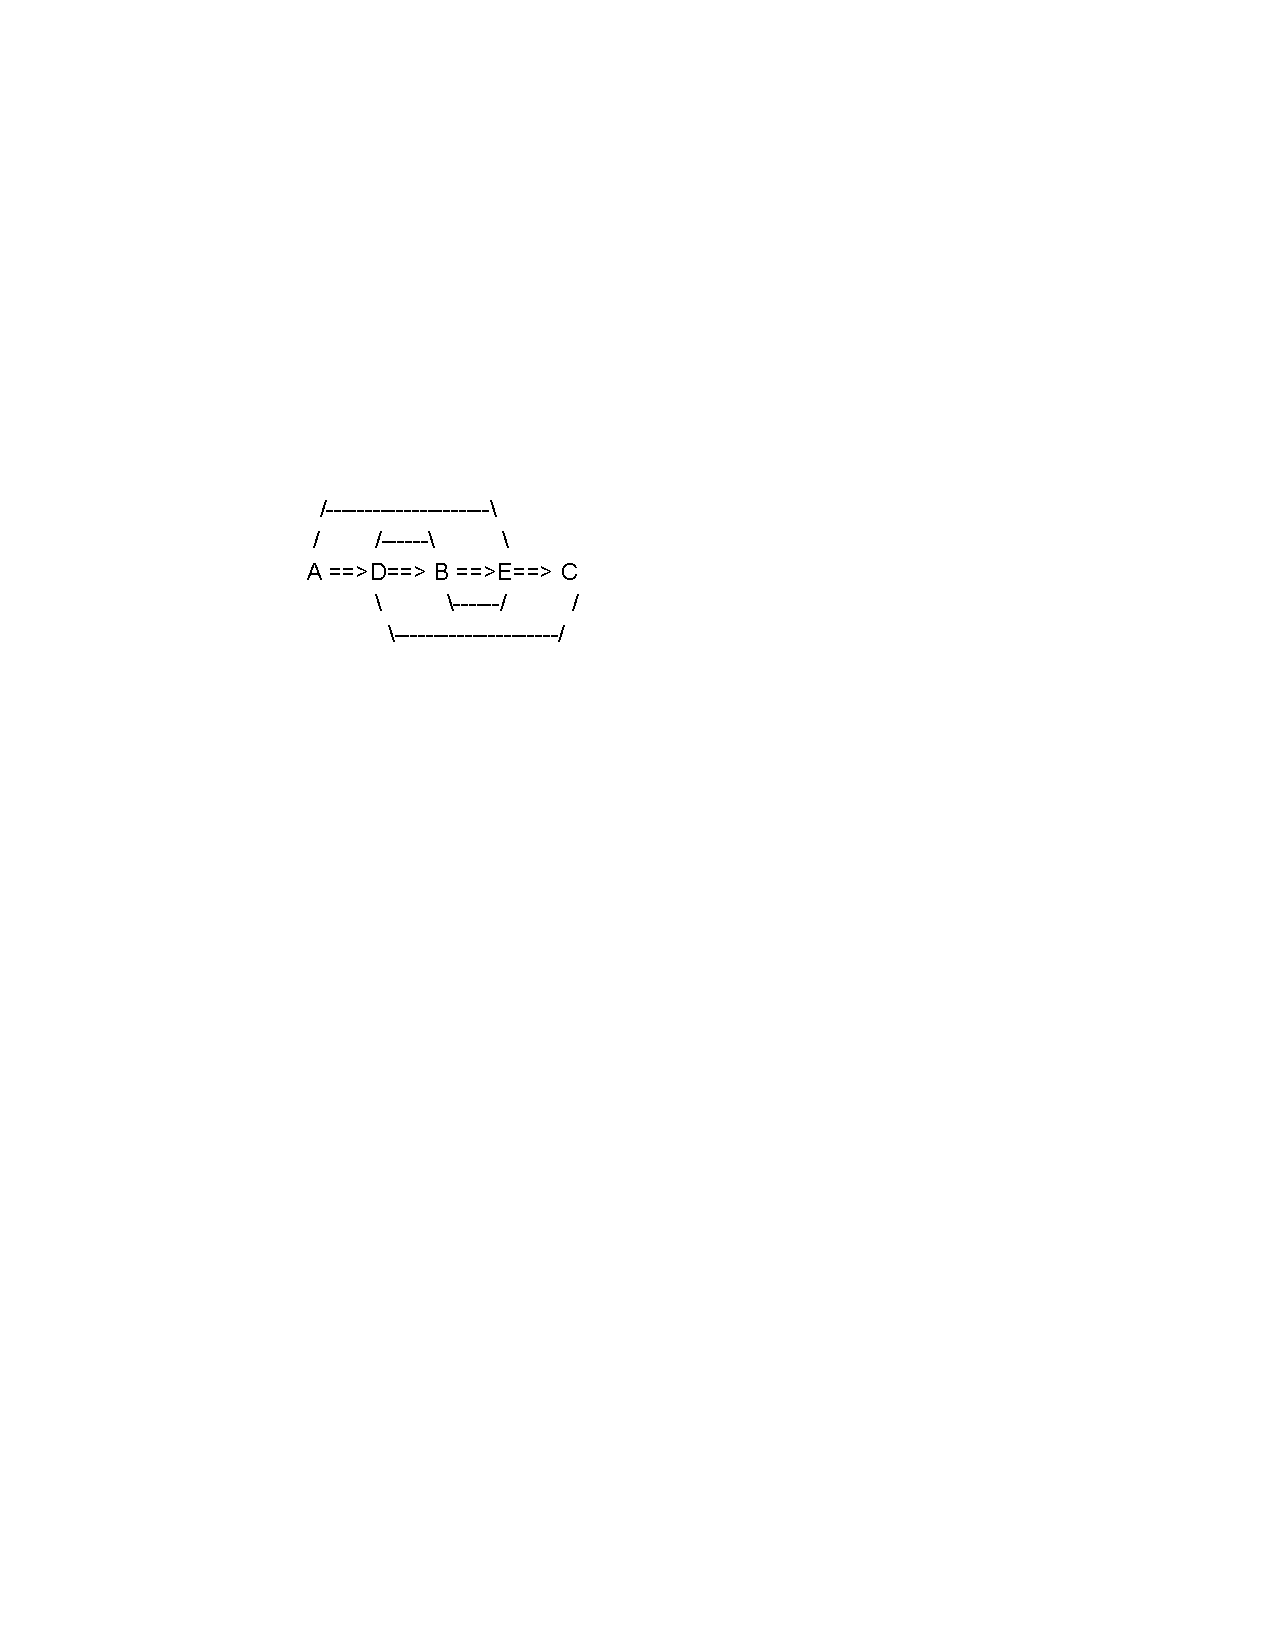
\includegraphics[]{figs/circular2}}
  \subfigure[case 3]{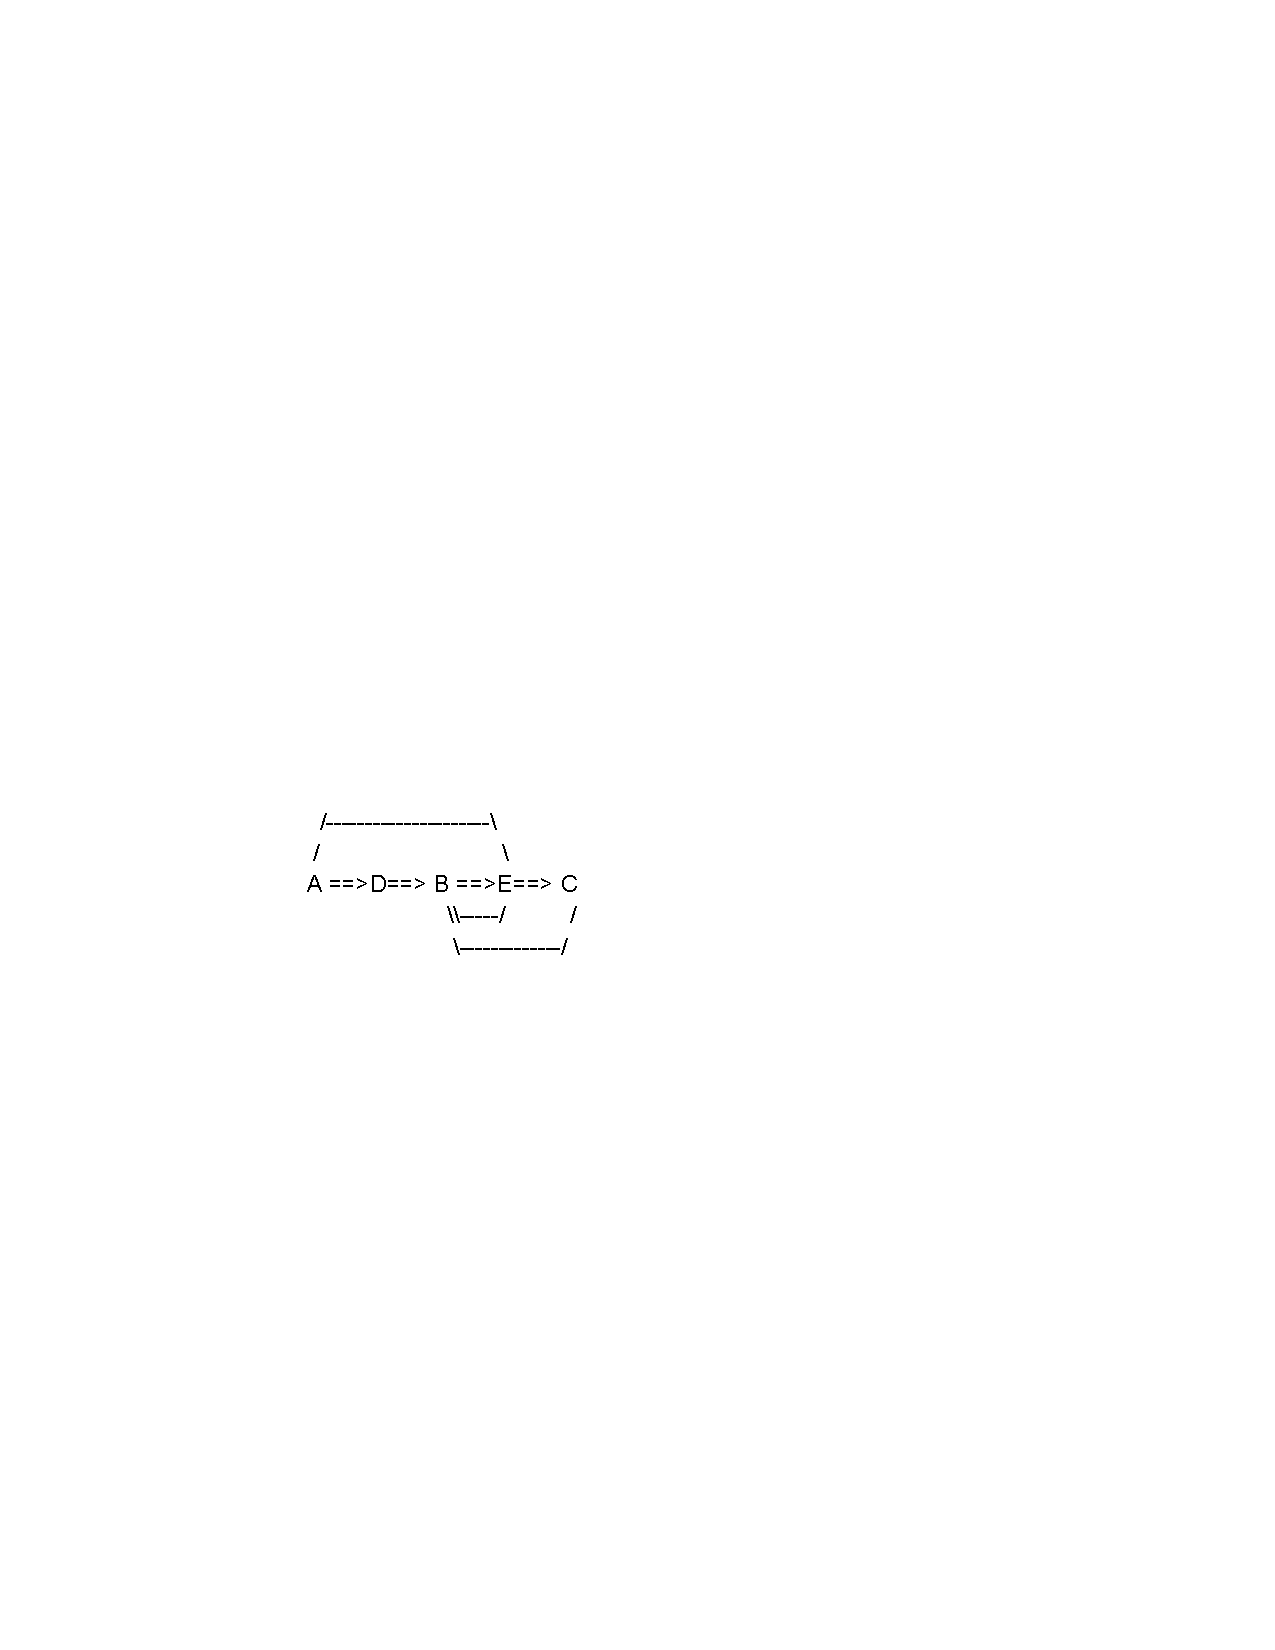
\includegraphics[]{figs/circular3}}
  \subfigure[case 4]{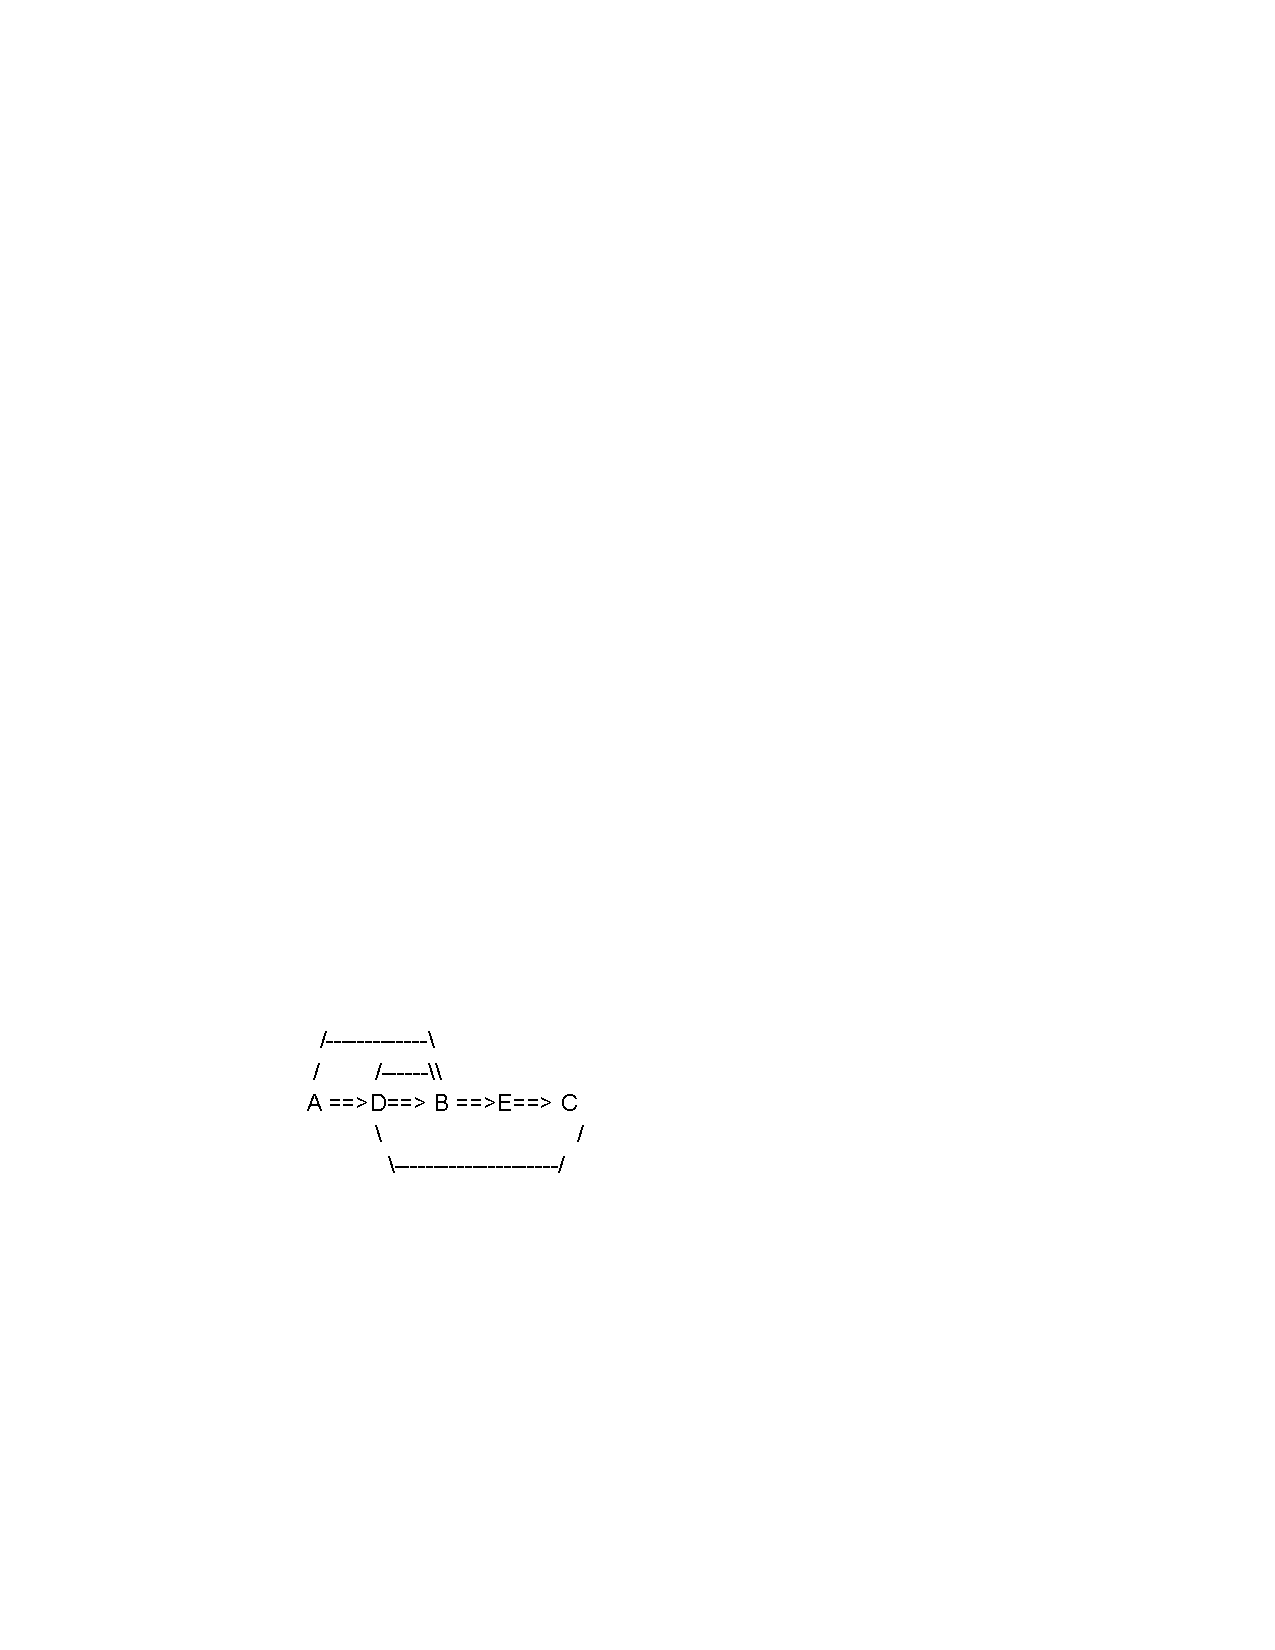
\includegraphics[]{figs/circular4}}
  \subfigure[case 5]{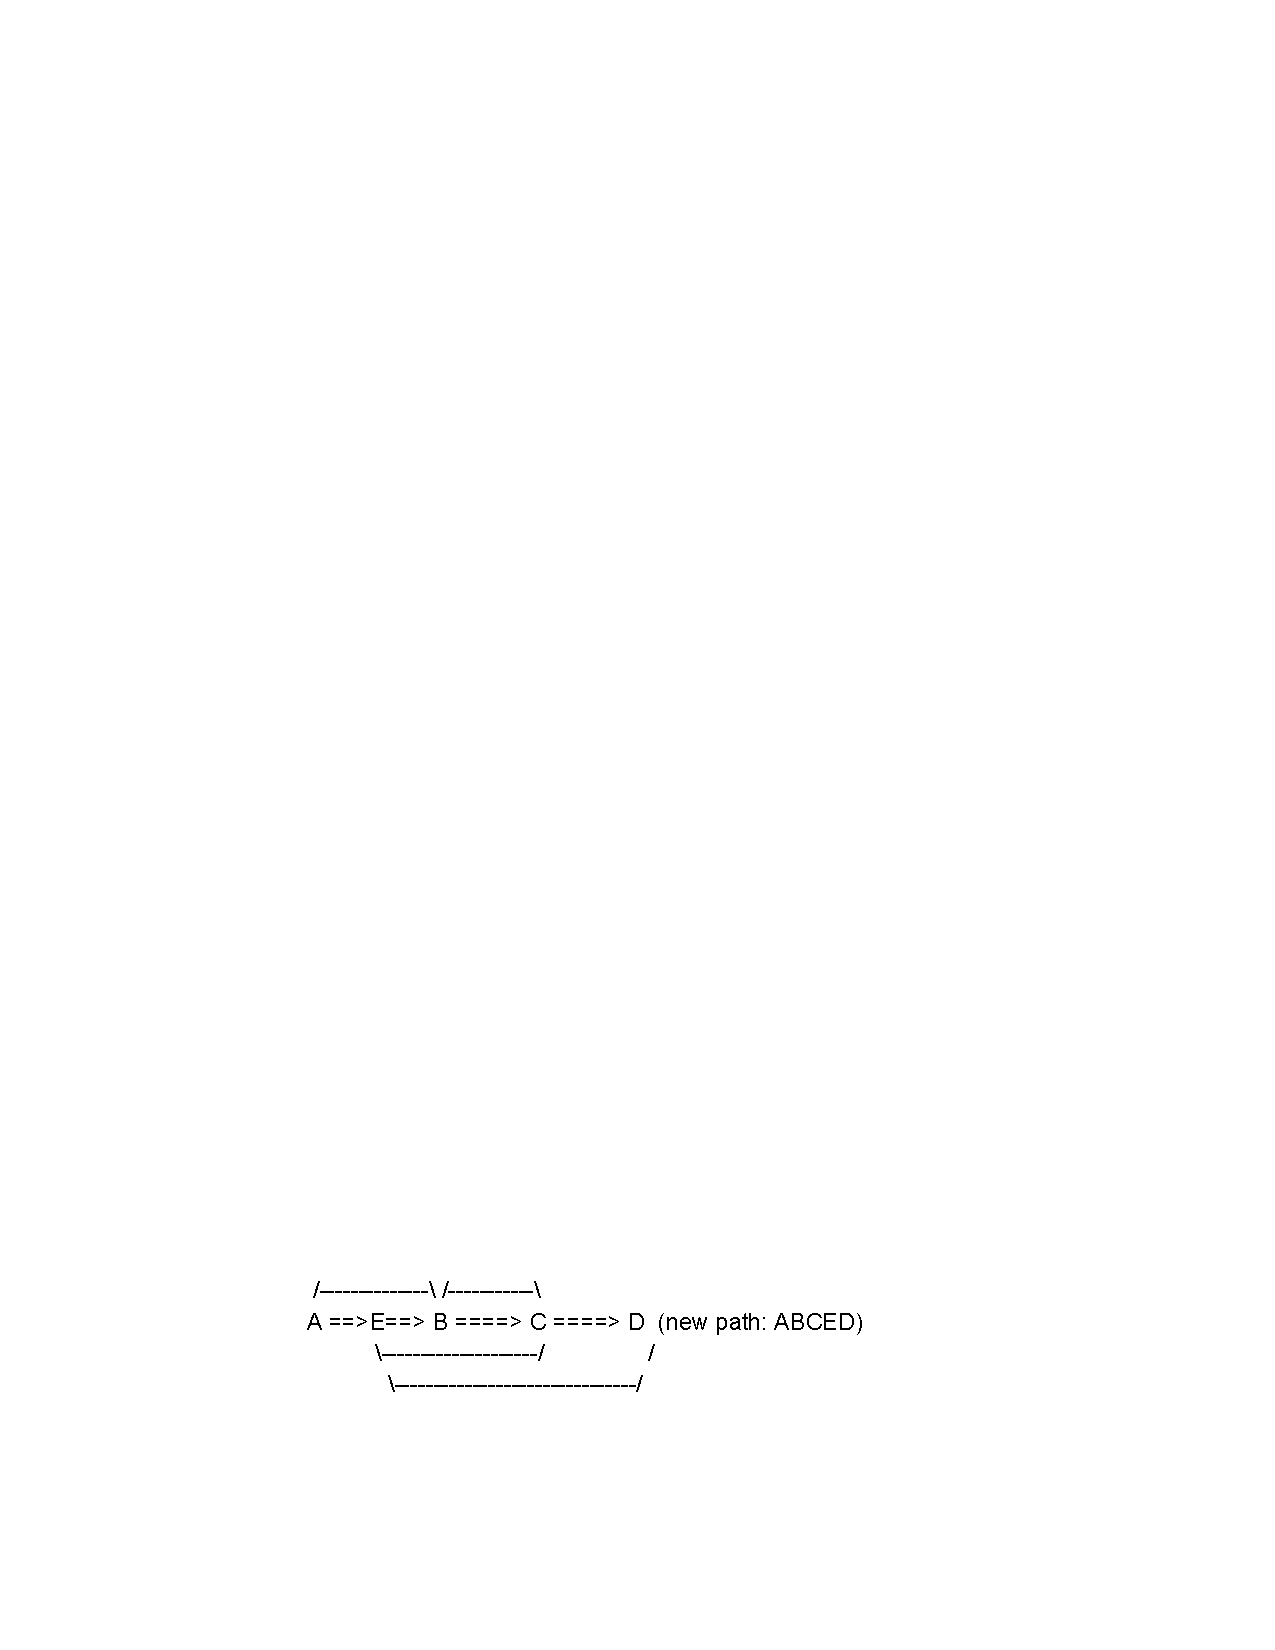
\includegraphics[]{figs/circular5}}
  %\vspace{10pt}
  \caption{\em \small Examples: circular dependencies between segments.}
  \label{fig:circular}
\end{figure}

\begin{theorem} (Conditions of the existence of an invariant complying update order): 
\begin{itemize}[noitemsep,topsep=0pt,leftmargin=*]
\item independent ECs, i.e., no overlapping updates across different ECs.
\item no circular dependencies between segments. 
In particular, if invariants are enforcing no more than two waypoints.
an update order always exists. 
\end{itemize} 
\end{theorem}

%\begin{proof}
%\end{proof}
\wxzc{need to prove it holds for multi-path?}

\paragraph{Other Categories?}

Overlapping ECs:
1. split updates to non-overlapping; 2. use mechanisms like consistent updates.

Slice isolation: If the output
of packet set of slice $a$ at any switch port, overlaps with any other slice,
then there is the potential for leaks. 

Multiple waypoints 

Path length constraint: Suppose
we wish to ensure that no flow from port $C$ to port $S$ should go through more
than 3 switches represents this check.

Quantitative properties (with SWAN)     
\fi                    

%\footnotesize
%{
\bibliographystyle{abbrv}

\setlength{\itemsep}{-2mm}
%\scriptsize
\bibliography{paper}
%}

\end{document}
